
\chapter{Molecular Crystal Global Phase Diagrams. II. Reverse Engineering the Intermolecular Potential}
\label{ch4} This chapter will be submitted for publication.
Richard McClurg has contributed to the work of identifying
non-canonical sphere packing reference lattices (everything but
bcc, fcc, hcp, sc, and diam), has written part of Section 3, and
has offered numerous helpful suggestions.

\begin{abstract}
Previously~\cite{Keith04c,Mettes04}, we developed a method for
constructing global phase diagrams for molecular crystals in which
crystal structure is presented as a function of intermolecular
potential parameters. These diagrams are useful for crystal design
and reverse engineering the intermolecular potential of an
experimentally observed crystal structure. We use this previous
method to reverse engineer a potential sufficient to produce the
structures of fully ordered single component crystals composed of
tetrahedral molecules in the Cambridge Structural Database. This is
significant because our prior work did not specify the number of
different molecular packings, called reference lattices, to
consider. Nor did it specify the number of parameters needed for the
diagrams. We find the structures of all tetrahedral molecules pack
in 15 reference lattices: bcc (25.7\%), fcc (24.3\%), A5 (8.6\%),
hcp (8.6\%), sc (8.6\%), and others (24.2\%). Although there are
suggestions in prior literature that thousands of parameters are
required to adequately describe tetrahedral molecule intermolecular
potentials,~\cite{Briels80} we find 15 parameters are sufficient to
successfully plot the structures of our test data on molecular
crystal global phase diagrams.
\end{abstract}


\section{Introduction}

Supramolecular organic solids and mesophases are of primary
interest in pharmaceuticals, electrophotographic processes,
organic pigments and dyes, and molecular FET's and
dielectrics~\cite{Bassoul00}. To alter their electrical, optical,
thermal, and solubility properties it is necessary to design both
the molecular and supramolecular structure to produce novel,
application-specific materials. While quantum methods are adequate
for predicting molecular properties, the weak interactions
responsible for determining supramolecular structure are more
difficult to design~\cite{Lommerse00,Motherwell02}.

Previously, we introduced a tool for exploring the molecular
parameter space of plastic and molecular crystals using a global
phase diagram (GPD)~\cite{Keith04c,Mettes04}. Global phase diagrams
summarize the phase behavior of a class of substances as a function
either of parameters in an empirical equation of state or of
parameters in an intermolecular potential. The classic example of a
GPD of the first type is the classification scheme for high pressure
vapor liquid phase equilibria by van
Konynenburg~\cite{VanKonynenburg80}. Their classification was based
on the van der Waals equation of state with simple binary mixing
rules. Despite the crude equation of state employed, it is still
widely used to classify the phase behavior of real binary mixtures.
Our GPD's are of the second type. They use an intermolecular
potential constructed from a complete set of basis functions for
rotational space for all molecules of a particular point group and a
set of molecular center-of-mass packings inferred from experimental
crystal structures. The parameters of the intermolecular potential
become axes on GPD's for each packing and the crystal structures are
phase regions in the diagrams.

An important benchmark of GPD's utility is to show that
experimentally observed structures can be found and their
intermolecular potential parameters read from the axes. Our goal
is to determine the number of translational packings, or reference
lattices, required in GPD construction and the number of potential
parameters needed to find all experimental phases.  A small number
of each will disprove previous hypotheses that many parameters are
needed~\cite{Briels80} and enhance the useability of GPD's in
materials design.

%In this paper we determine potential parameters for
%single-component tetrahedral molecules in the Cambridge Structural
%Database (CSD)~\cite{Allen02}.  We first identify the
%high-symmetry lattice formed by the molecular centers of each
%experimental structure. This gives us a starting point or
%reference lattice from which GPD's were constructed previously.
%The rotational potential is then expanded in a complete set of
%basis functions whose potential coefficients are independent
%variables on GPD's.  In this paper however we map these to the
%n-sphere and search among them for the correct or observed crystal
%structure.  This is done using global optimization techniques
%among parameter \emph{and} configurational space.

The outline of the balance of the paper is as follows. In
Sec.~\ref{Reference_Phases} we discuss the derivation of our data
set, its chemical and crystallographic characteristics, and group
entries based on structural similarity. In Sec.~\ref{assignments} we
deduce reference lattices for each structure by pseudo-symmetry
detection and describe the fit of the structures to these lattices.
In Sec.~\ref{method} we review the rotational potential and outline
the computational procedure to find the potential parameters for
each structure. In Sec.~\ref{discussion} we discuss and visualize
the reverse-engineered potentials for tetrahedral molecules in the
CSD and discuss features and limitations of the model.

\section{Experimental Data Set}
\label{Reference_Phases}

\begin{landscape}
\begin{table}
\caption{Identifiers, chemical formulas, and names of the
tetrahedral data set.}\label{names1} \tiny
\begin{tabular}{llll}
Identifier & formula & name & framework\\
\hline
ADAMAN08 & C10 H16 & Adamantane & adamantane \\
BASXOI & C4 H12 Se6 Sn4 & 1,3,5,7-Tetramethyl-2,4,6,8,9,10-hexaselena-1,3,5,7-tetrastanna-adamantane & adamantane \\
BOGMEP & C24 H48 Cl6 Cu4 N16 O1 & hexakis($M_2$-Chloro)-($M_4$-oxo)-tetrakis(hexamethylenetetramine-copper(ii)) & other \\
CAMPOV & C16 H36 N4 Sn4 & tetrakis(($M_3$-t-Butylimino)-tin) & cubane\\
CANFIG & C4 H24 B4 U1 & tetrakis(Methyltrihydroborato)-uranium(iv) & MX$_4$\\
CANFOM & C4 H24 B4 Th1 & tetrakis(Methyltrihydroborato)-thorium(iv) & MX$_4$\\
CARBTC & C1 Cl4 & Carbon tetrachloride & MX$_4$\\
CARBTC07 & C1 Cl4 & Carbon tetrachloride & MX$_4$\\
CTBROM & C1 Br4 & Carbon tetrabromide & MX$_4$\\
CUCZUV & C20 H36 & Tetra-t-butyltetrahedrane & tetrahedrane\\
DEQPAQ & C36 H100 B4 N12 Na4 & tetrakis(($M_3$-Tetrahydroborate-H,H,H)-pentamethyldiethylenetriamine-sodium) & other\\
DILWIE01 & C16 H48 Pt4 S4 & tetrakis(($M_3$-Methylsulfido)-trimethyl-platinum(iv)) & cubane\\
DOCNIS & C8 H12 S6 & 1,3,5,7-Tetramethyl-2,4,6,8,9,10-hexathia-adamantane & adamantane\\
FOHCUA & C12 Ni4 O18 P4 & P,P',P'',P'''-tetrakis(Tricarbonyl-nickel)-tetraphosphorus-hexaoxide & adamantane\\
FOJBUB02 & C4 Ni1 O4 & Tetracarbonyl-nickel & MX$_4$\\
FUZLUH & C12 Co4 O12 Sb4 & tetrakis(Tricarbonyl-($M_3$-stibido)-cobalt) & cubane\\
FUZTEZ & H16 B4 Np1 & tetrakis(Tetrahydroborato)-neptunium(iv) & MX$_4$\\
FUZVOL & H16 B4 Hf1 & tetrakis(Tetrahydroborato)-hafnium & MX$_4$\\
GERHOA & C4 H12 Cl12 N4 Sb4 & 1,3,5,7-Tetramethyl-2,2,2,4,4,4,6,6,6,8,8,8-dodecachloro-1,3,5,7 & cubane\\
&&-tetra-aza-2,4,6,8-tetrastibapentacyclo(4.2.0.0$^2,5$.0$^3,8$.0$^4,7$)octane \\
GUTCED & C26 H32 & (1(2,3)4)Pentamantane & other\\
HMGETP & C12 H36 Ge6 P4 & hexakis(Dimethylgermanium)tetraphosphide & adamantane\\
HMSIPA & C12 H36 P4 Si6 & Dodecamethyl-hexasila-tetraphospha-adamantane & adamantane\\
HXMTAM07 & C6 H12 N4 & Hexamethylenetetramine & adamantane\\
JEYSEL & C18 H36 Ni4 O6 P4 & hexakis($M_2$-Carbonyl)-tetrakis(trimethylphosphine)-tetra-nickel & tetrahedrane\\
JUFWUC & C12 H40 Cs4 N4 Si4 & tetrakis($M_3$-Trimethylsilylamido)-tetra-cesium cubane & cubane\\
KANGUB01 & C10 H12 I4 & 1,3,5,7-Tetraiodo-adamantane & adamantane\\
KELREY & C12 H36 Cl4 Ti4 & tetrakis($M_3$-Chloro)-tetrakis(trimethyl-titanium) & cubane\\
KOXKOX & C16 H36 Ga4 Se4 & tetrakis(($M_3$-Selenido)-t-butyl-gallium) & cubane\\
KUJSIR & C20 H48 O4 Zn4 & tetrakis($M_3$-t-Butoxo)-tetrakis(methyl-zinc) & cubane\\
LUFYEQ & C12 H12 Si1 & tetrakis(Prop-1-ynyl)silane & MX$_4$\\
MECKIO & C16 H36 Cl4 In4 N4 & tetrakis($M_3$-t-Butylimido)-tetrachloro-tetra-indium & cubane\\
MECKOU & C16 H36 Br4 In4 N4 & tetrakis($M_3$-t-Butylimido)-tetrabromo-tetra-indium & cubane\\
MECKUA & C16 H36 I4 In4 N4 & tetrakis($M_3$-t-Butylimido)-tetraiodo-tetra-indium & cubane\\
MESIAD & C12 H36 As4 Si6 & Dodecamethyl-hexasila-tetra-arsa-adamantane & adamantane\\
MEZDIE01 & C12 H36 Si1 Sn4 & tetrakis(trimethylstannyl)silane & MX$_4$\\
MEZDOK01 & C12 H36 Ge1 Sn4 & tetrakis(trimethylstannyl)germane &
MX$_4$
\end{tabular}
\end{table}
\end{landscape}

\begin{landscape}
\begin{table} \tiny
\begin{tabular}{llll}
Identifier & formula & name & framework\\
\hline
MPTHOT01 & C12 H40 O4 Pt4 & tetrakis(($M_3$-Hydroxo)-trimethyl-platinum) & cubane \\
MSISUL10 & C4 H12 S6 Si4 & Tetra(methylsilicon)-hexasulfide & adamantane\\
MTRETC10 & C16 H12 O12 Re4 S4 & tetrakis(Tricarbonyl-$M_3$-methanethiolato-rhenium) & cubane\\
MXSNOX & C4 H12 O8 Sn6 & tetrakis($M_3$-Methoxy)-tetrakis($M_3$-oxo)-hexa-tin & other\\
MZNMOX10 & C8 H24 O4 Zn4 & tetrakis(($M_3$-Methoxo)-methyl-zinc) & cubane\\
NIWMIP & C12 H36 Al4 N4 S6 & hexakis($M_2$-Sulfido)-tetrakis(trimethylamide)-tetra-aluminium & adamantane\\
OHABEE & C16 H36 Si4 & tetrakis(Trimethylsilyl)tetrahedrane & tetrahedrane\\
POSLOY10 & C12 Cl4 O12 Tc4 & tetrakis(($M_3$-Chloro)-tricarbonyl-technetium) & cubane\\
QUGBOJ & C16 O16 Rh6 & tetrakis($M_3$-Carbonyl)-dodecacarbonyl-hexa-rhodium & other\\
RASDOE & C16 H48 Ga4 N4 Si4 & tetrakis($M_3$-Trimethylsilylimido)-tetramethyl-tetra-gallium(iii) & cubane\\
REKYUB & C16 H36 Ga4 S4 & tetrakis(($M_3$-Sulfido)-t-butyl-gallium) & cubane\\
RIMMOP & C16 H40 Al4 N4 & tetrakis(($M_3$-t-Butylamido)-hydrido-aluminium) & cubane\\
RIMNAC & C20 H48 Al4 N4 & tetrakis(($M_3$-t-Butylamido)-methyl-aluminium) & cubane\\
RUQMEV & C12 H36 Cu4 I4 N4 & tetrakis($M_3$-Iodo)-tetrakis(trimethylamino)-tetra-copper(i) & cubane\\
SENLAY & C16 H36 P4 Si4 & 2,4,6,8-Tetra-t-butyl-1,3,5,7-tetraphospha-2,4,6,8-tetrasila-pentacyclo(4.2.0.0$^2,5$.0$^3,8$.0$^4,7$)octane & cubane\\
TCYMET & C5 N4 & Tetracyanomethane & MX$_4$\\
TFMETH02 & C1 F4 & Carbon tetrafluoride & MX$_4$\\
TMEPTC & C12 H36 Cl4 Pt4 & tetrakis(($M_3$-Chloro)-trimethyl-platinum) & cubane\\
TMGEHS10 & C4 H12 Ge4 S6 & Tetra(methyl-germanium) hexasulfide & adamantane\\
TMSIAD & C10 H24 Si4 & 1,3,5,7-Tetramethyl-tetrasila-adamantane & adamantane\\
TMSNHS10 & C4 H12 S6 Sn4 & Tetra(methyltin) hexasulfide & adamantane\\
TOHSUE & C16 F12 O12 P4 Ru4 & tetrakis(($M_3$-Trifluoromethylphosphido)-tricarbonyl-ruthenium) & cubane\\
VADRAU & C4 H12 Pb1 & Tetramethyl-lead(iv) & MX$_4$\\
VAFWAA & C12 Bi4 Co4 O12 & tetrakis(Tricarbonyl-($M_3$-bismuth)-($M_3$-cobalt)) & cubane\\
VAVYAS & C20 H36 P4 & 2,4,6,8-Tetra-t-butyl-1,3,5,7-tetraphosphacubane & cubane\\
XAGXAE & P4 S10 & 2,4,6,8,9,10-Hexathia-1,3,5,7-tetraphosphatricyclo(3.3.1.1$^3,7$)decane 1,3,5,7-tetrasulfide & adamantane\\
XUWROW & C20 H48 Mg4 O4 & tetrakis($M_3$-t-Butoxo)-tetramethyl-tetra-magnesium & cubane\\
YEMRIR & O6 P4 S4 & 2,4,6,8,9,10-Hexaoxa-1,3,5,7-tetraphosphatricyclo(3.3.1.1$^3,7$)decane 1,3,5,7-tetrasulfide & adamantane\\
YEYQAU & C12 O12 Ru4 Se4 & tetrakis(($M_3$-Selenido)-tricarbonyl-ruthenium) & cubane\\
YIMWEW & C10 H16 O4 & 1,3,5,7-Tetrahydroxyadamantane & adamantane\\
ZEYHIU & C20 H48 Cd4 O4 & tetrakis(($M_3$-t-Butoxo)-methyl-cadmium) & cubane\\
ZIZHIZ & C12 H4 Mn4 O16 & tetrakis(($M_3$-Hydroxo)-tricarbonyl-manganese) & cubane\\
ZNOXAC01 & C12 H18 O13 Zn4 & hexakis($M_2$-Acetato-O,O')-($M_4$-oxo)-tetra-zinc & other\\
ZZZKDW01 & C1 I4 & Carbon tetraiodide & MX$_4$\\
\hline
\end{tabular}
\end{table}
\end{landscape}

Since our molecular crystal global phase diagrams are constructed
for molecules of a given molecular point group symmetry, we have
chosen to use the \emph{CSDSymmetry} database as our primary source
of crystal structures~\cite{Yao02}. This database summarizes the
point groups of molecules that form error-free, nonpolymeric,
nonionic, coordinate-determined molecular crystals in the CSD.
Duplicates were removed from the database and hydrogen atoms were
not considered when assigning point groups. While the methods
introduced in our previous work~\cite{Mettes04} are applicable to
disordered structures, which are systematically absent from
\emph{CSDSymmetry}, it is a convenient source of crystal data for
molecules of a particular point group. Our methods are restricted to
single component crystals, however. Therefore we worked with the
single component crystal subset of the \emph{CSDSymmetry} database.
This was accomplished by first querying the CSD for all single
component crystals using {C\small ONQUEST}, the interface to the
CSD, and then using {C\small ONQUEST} to take the intersection of
the two data sets.

Continuing the example begun in our prior work~\cite{Mettes04}, we
chose to consider crystals composed of molecules with T$_d$
molecular point group symmetry.  We have augmented the data from
\emph{CSDSymmetry} with a recently determined structure of the low
temperature ordered phase of heavy methane~\cite{Neumann03}.  The
data set contains 71 crystal structures of 70 different chemical
substances.  Only carbon tetrachloride ($\mathrm{CCl}_4$) appeared
twice in different polymorphs. [CSD structures
CARBTC~\cite{Piermarini73} and CARBTC07~\cite{Cohen79}]. Names and
chemical formulas for all the entries are given in
Table~\ref{names1}. The chemical structures include 15 hydrocarbons
and their substituted derivatives and 56 organometallics. The
organometallics contain 30 different metals: Al, As, Bi, Cd, Co, Cs,
Cu, Ga, Ge, Hf, In, Mg, Mn, Na, Ni, Np, Pb, Pt, Re, Rh, Ru, Sb, Si,
Se, Sn, Tc, Th, Ti, U, and Zn. Eight types of molecular frameworks
are present in the data set: Cubane (29), Adamantane (17), MX$_4$
(16), Tetrahedrane (3), and others (6). There are entries from all
seven crystal systems in the data set. Twenty crystals are cubic (or
isometric), one is hexagonal, five are trigonal, ten are tetragonal,
six are orthorhombic, 22 are monoclinic, and seven are triclinic as
shown in Fig.~\ref{distro}. This distribution is different than the
CSD as a whole~\cite{Bauer92}, but that is not surprising given the
larger-than-average number of symmetries in the T$_d$ point group.
The data set is sufficient however to test whether molecular crystal
global phase diagrams apply to hydrocarbons and organometallics, a
variety of molecular frameworks, and all seven crystal systems.

\begin{figure}
\begin{center}
\scalebox{.7}{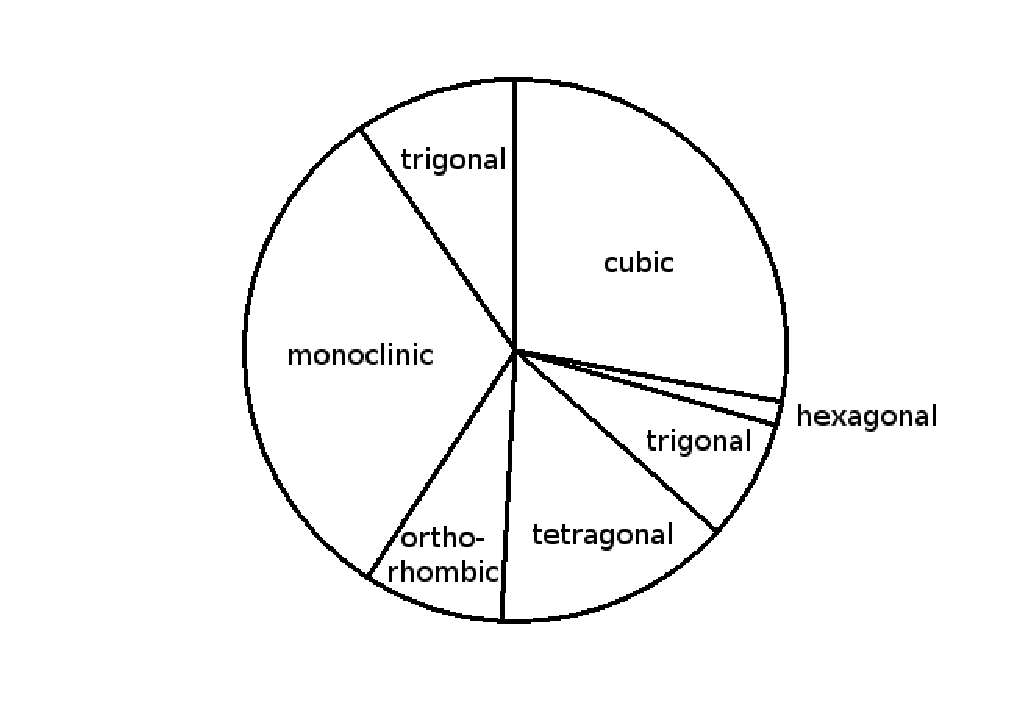
\includegraphics{crystalSystems.eps}}
%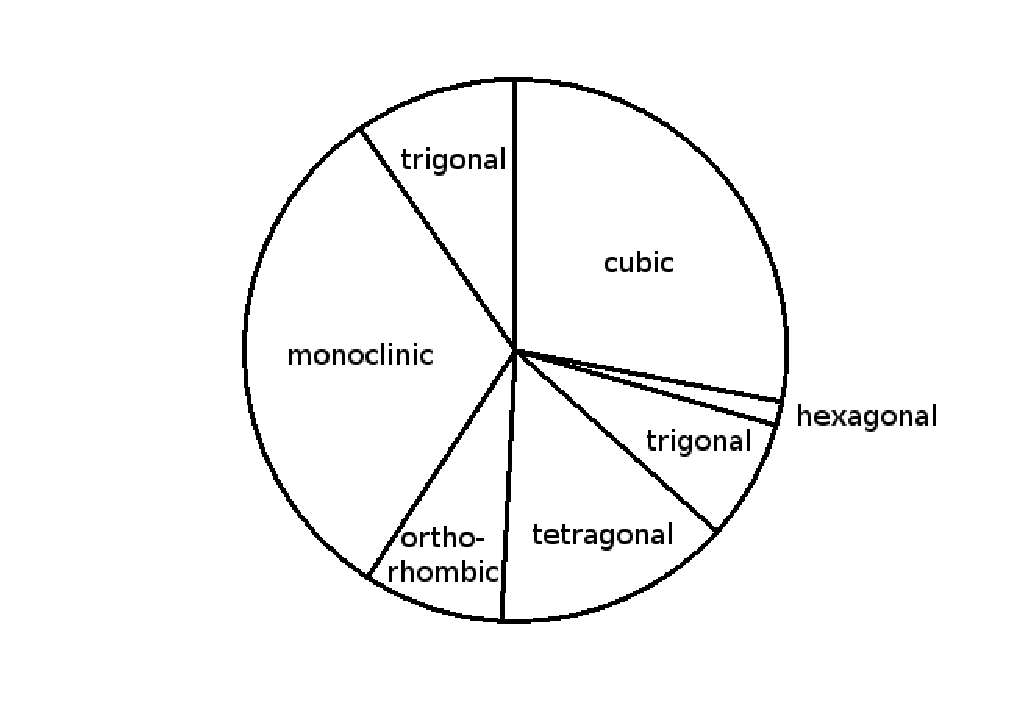
\includegraphics{crystalSystems.eps}
\caption[Distribution of experimental structures among the seven
crystal systems.]{Crystal systems for crystals of tetrahedral
molecules.\label{distro}}
\end{center}
\end{figure}

One entry [CSD structure XUWROW~\cite{sung02}] is a very unusual
structure containing 70\% voids as recorded by the CCDC staff in
its cif file in the CSD, presumably using the standard van der
Waals radii in the documentation of CCDC software~\cite{Bruno02}.
It was grown as a thin epitaxial crystal under ultra-high vacuum.
Apparently the crystal structure is strongly influenced by the
substrate and we exclude it from further consideration.


The remaining crystal structures were organized into groups that
bear a strong ``structural relation'' as discussed in the
International Tables for Crystallography (ITC)~\cite{Hahn83}. For
crystals to belong to the same group they must have the same space
group symmetry, cell lengths in similar proportions, similar cell
angles, and molecular centers at equivalent Wyckoff point(s) with
similar structural parameter values where applicable.  We refer to
these groups as sharing a particular distinct structure. Note that
we do not require that the atomic positions be similar to be
classified in the same distinct structure. For example, two
structures [CSD structures DILWIE01~\cite{Ebert98} and
ZEYHIU~\cite{Noth95}] crystallize in space group 165 with molecules
at Wyckoff point d. Their cell parameters are also in similar
ratios. Therefore, we classify them in the same distinct structure,
despite their different chemical structures with different numbers
of atoms.

Two structures in \emph{CSDSymmetry} [CSD structures
HMGETP~\cite{Dahl75} and JUFWUC~\cite{Tesh92}] have molecules that
are tetrahedral within the default error bounds for detecting
molecular symmetry, but are sufficiently distorted to influence
their space group classifications (195a and 197a, respectively).
Either the molecules are very slightly distorted in the crystal or
the crystal symmetries are under-specified and actually belong to
space groups 215 and 217, respectively. Although slight
distortions could result from crystal Jahn-Teller distortions, for
example, we adopt the later interpretation. Therefore these
crystals have been grouped with distinct structures 215a and 217a,
respectively. This assignment is discussed from an energetic point
of view in Sec.~\ref{discussion}.

The 70 crystal structures fell into 46 distinct structures. Five
structures are cubic (or isometric), one is hexagonal, four are
trigonal, eight are tetragonal, six are orthorhombic, sixteen are
monoclinic, and six are triclinic. These distinct structures are
further characterized in the following section.

\section{Reference Lattice Assignments}
\label{assignments}

Our global phase diagrams are constructed starting with a fully
disordered plastically crystalline reference state.  At
sufficiently high temperature the intermolecular potential, which
hinders free rotation, becomes weaker than the thermal energy.  In
this limit molecules are free to disorder and ultimately to freely
rotate. Since the molecules are disordered they may occupy high
symmetry Wyckoff points in high symmetry space groups. These are
space groups with special values of the cell parameters
$(a,b,c,\alpha,\beta,\gamma)$ and molecules located at special
values of the unit cell fractional coordinates (x,y,z). Each
molecule has four or more generally equivalent non-coplanar
nearest neighbors. This is needed for structural stability in
three dimensions. We call these reference lattices.

High symmetry reference lattices may be determined for an
experimental crystal structure by determining the space group formed
from the lattice of the molecular centers of mass. These
calculations were done using F{\small INDSYM} in the I{\small
SOTROPY} software suite~\cite{Stokes02b} with coordinates scaled by
the minimum unit cell length $\{a,b,c\}$ and a large error tolerance
setting (0.1). Initially it may seem unexpected that molecular
crystals, the majority of which belong to monoclinic or triclinic
space groups~\cite{Bassoul00}, should be slight distortions of high
symmetry lattices. However, prior work in this area has shown this
is not only possible but quite
common~\cite{Motherwell97,Reichling00}. Standard unit cell choices
for low symmetry crystals systems often hide the similarity of a
suitably-chosen supercell to a reference lattice in a higher
symmetry crystal system. This high translational symmetry is a
result of the close-packing tendency of molecules. Broken symmetries
are due to orientational ordering and anisotropic intermolecular
potentials.

Occasionally a structure arises with fewer than four nearest
neighbors per molecule.  Due to the inherent lack of structural
stability of this arrangement, this suggests the crystal is in fact
a lattice of molecular clusters, typically \emph{dimers}, acting as
a single entity.  In such a case the center of mass of the dimers is
used in F{\small INDSYM} again with a larger error tolerance.

Given a list of common reference lattices, we developed an automated
technique to identify the reference lattices of experimental
structures. From a list of possible reference lattices, we
superimpose an experimental structure on each possible lattice so
one molecule in each structure overlaps. Then the experimental
structure is rotated and isotropically scaled in order to minimize
the sum of the absolute values between the center of each molecule
of the experimental structure and the center of the closest
reference lattice molecule,
\begin{equation}
\min_{a,\mbss{\omega}}\sum_m|\mb{R}(a,\mb{\omega})\cdot\mb{X}^{\mathrm{exp}}_m
 - \mb{X}^{\mathrm{ref}}_{\mathrm{closest}}|,
\end{equation}
where $\mb{R}(a,\mb{\omega})$ is a Cartesian rotation matrix
multiplied by an isotropic scaling factor $a$
(Appendix~\ref{cartRot}), $\mb{X}^{\mathrm{exp}}_m$ is the center
of mass of a molecule in the experimental structure,
$\mb{X}^{\mathrm{ref}}_{\mathrm{closest}}$ is the center of mass
of the closest molecule in one of the possible reference lattices,
and $m$ sums over all molecules in the experimental structure,
which is typically limited to the first 14 neighbors of the
superimposed center molecule.  This cutoff is justified by CSD
studies~\cite{Peresypkina00} showing 14 to be the most common
molecular coordination number. This technique was used in a
computer program to identify the majority of the fcc, bcc, hcp,
sc, and diamond reference lattices.

Applying these techniques to our data set gives the reference
lattice assignments in Tables~\ref{cubic}-~\ref{mono}. Generally we
name reference lattices first by their common name (\emph{i.e.} fcc)
if available, then by their Strukturbericht designation (\emph{i.e.}
A15) if available, and then by their space group/filled Wyckoff
positions if necessary (\emph{i.e.} 70a).  The raw atomic positions,
symmetry operators, etc. contained in the cif and fdat data files
from the CSD were processed using the cctbx collection of
algorithms~\cite{Grosse-Kunstleve02}. Algorithms from the I{\small
SOTROPY} software suite~\cite{Stokes02b} and the Bilbao
Crystallographic Server~\cite{Kroumova03} were also used to identify
group-subgroup relations, track Wyckoff point evolution, etc. In the
following subsections we review the reference lattices for the
structures in the experimental data set.

\subsection{Cubic (Isometric) Space Groups}

The cubic crystal structures are summarized in Table~\ref{cubic}.
%Note that we use
%the space group designations of the 1983 version of ITC instead of
%the recent and less well-known edition~\cite{Hahn02}.
Each structure is listed as a space group number followed by its
occupied Wyckoff points. A representative of each structure is named
in the next column.  Under each representative structure is  the
reference lattice. In the third column is shown the ratio $|G|/Z$.
This is the number of symmetry operations $|G|$ per molecules in the
unit cell $Z$. We call this ratio the symmetry density of a crystal
structure. Defined in this way, the symmetry density is independent
of the choice of unit cells. For instance the primitive and
conventional fcc cells both have $|G|/Z=48$. The symmetry density is
a maximum of 48 for fcc, bcc, and sc sphere packings. Symmetry
breaking, by loss of a class of symmetry operations and/or loss of
translations, reduces the symmetry density. The index $[i]$ of a
group-subgroup relation is the ratio of $|G|/Z$ of the group and its
subgroup. Thus, the geometric interpretation of the index is the
amount by which the symmetry of the crystal is diluted by symmetry
breaking (ITC, p726)~\cite{Hahn83}. The number of entries bearing a
strong structural similarity to the representative is shown in the
fourth column. For example, structure 217a has space group 217 with
molecules situated at Wyckoff point a. Its representative is DEQPAQ
and in a disordered state the crystal has the bcc symmetry or
reference lattice. Its symmetry density is 24 and that of its
reference lattice 48. Therefore, its index in bcc is 2. There are 11
tetrahedral molecular crystals in \emph{CSDSymmetry} with this
structure.

\begin{table}
\caption{Reference lattices for cubic (isometric) structures.}
\label{cubic}
\begin{center}
\begin{tabular}{cccc}%\hline
\cline{1-4}
Structure & Example & $|G|/Z$ & Entries \\
        & Lattice \\
\cline{1-4}
227a    & ZNOXAC01 & 24 & 1 \\
        & diam     & 24 \\
217a    & DEQPAQ   & 24 & 11 \\
        & bcc      & 48 \\
215a    & FOHCUA   & 24 & 3 \\
        & sc       & 48 \\
205c    & FOJBUB02 &  3 & 2 \\
        & d-fcc$^*$& 24 \\
218a,c  & SENLAY   &  3 & 3 \\
        & A15      &  6 \\
\cline{4-4}
\multicolumn{3}{r}{total:} & 20 \\
\cline{1-4}
\end{tabular} \\
$^*$ dimer packing
\end{center}
\end{table}

The 20 crystal structures in Table~\ref{cubic} fall into five
distinct structural types listed in order of decreasing symmetry
density. Structure 227a is unique in that the Wyckoff point
symmetry in the reference lattice is consistent with $T_d$
molecular point group symmetry. Therefore the (ordered)
experimental structure has the full symmetry of the (disordered)
reference lattice. Structures 217a and 215a are subgroups of bcc
and sc, both of index two. The molecular symmetry ($T_d$) is a
subgroup of the Wyckoff site symmetry in the reference lattice
($O_h$). Thus the crystal symmetry is reduced by molecular
ordering. Structure 218a,c is similarly a subgroup of index two of
A15, but the molecules on the two occupied Wyckoff sites are
inequivalent, even in the reference lattice.  For each of the
preceding structures, there are no arbitrary cell parameters or
structural parameters. Thus the molecular centers of mass coincide
exactly with the reference lattice.


\begin{figure}
\begin{center}
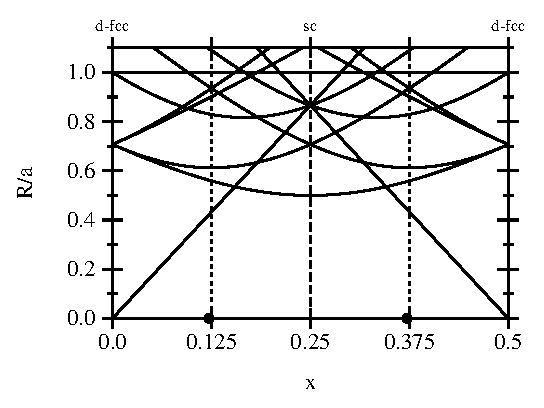
\includegraphics{205c.eps}
\end{center}
\caption[Neighbor distances for 205c as a function of $x$]{Neighbor
distances for 205c as a function of the Wyckoff structural
parameter, $x$.  The experimental structures, marked with circles,
are midway between the sc and doubly-occupied fcc limits.}
\label{fig:205c}
\end{figure}

Structure 205c has one arbitrary parameter, $x$, for its occupied
Wyckoff point.  This is called a Wyckoff structural parameter.
Figure~\ref{fig:205c} shows the neighbor distances as a function
of the structural parameter. The representative experimental
structure [tetracarbonyl-nickel CSD structure
FOJBUB02~\cite{Braga93}] has molecules at Wyckoff point c with a
structural parameter $x=0.122$ which is approximately midway
between the sc limit ($x=1/4$) and a doubly occupied fcc limit
($x=0$ or $1/2$). It is evident from the figure that the crystal
structure is equivalent for structural parameters $x$ and $1/2-x$.
Since the neighbor distances at the experimental values of the
structural parameter are qualitatively different than in the sc
lattice, the simple cubic reference lattice is not acceptable for
our purposes. The crystal is best viewed as a dimer packing with
dimer centers of mass on an fcc lattice as shown in
Fig.~\ref{dimers} for a dimer situated on the $(1/2,1/2,0)$ fcc
coordinate. Its three-fold axis is parallel to the body diagonal
direction. The dimer has point group symmetry $D_{3d}$ so we would
expect to identify this structure on a $D_{3d}$ global phase
diagram using an fcc reference lattice. This possibility is not
pursued further here.

\begin{figure}
\begin{center}
\scalebox{1}{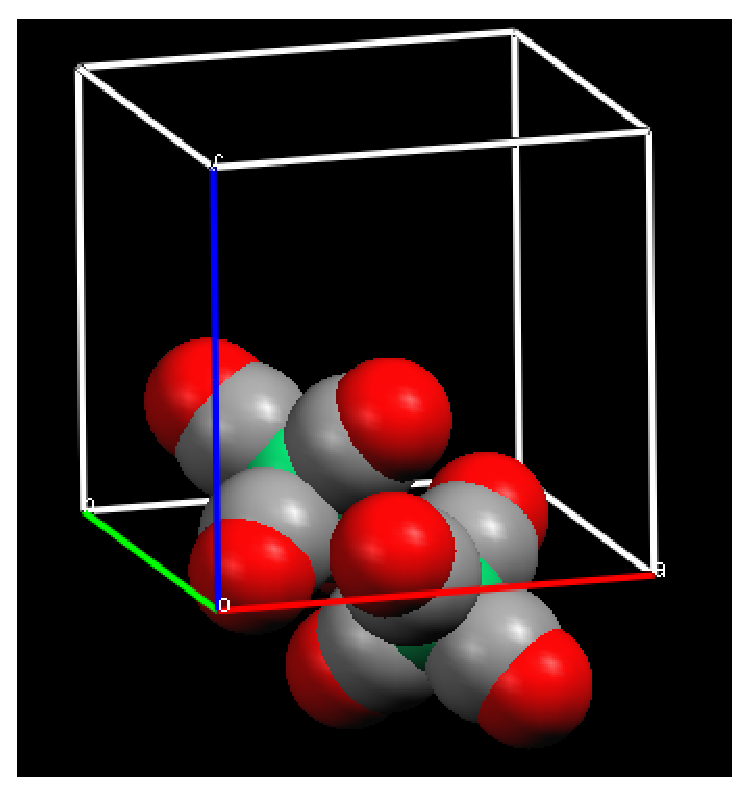
\includegraphics{FOJBUB02_Show.eps}}
%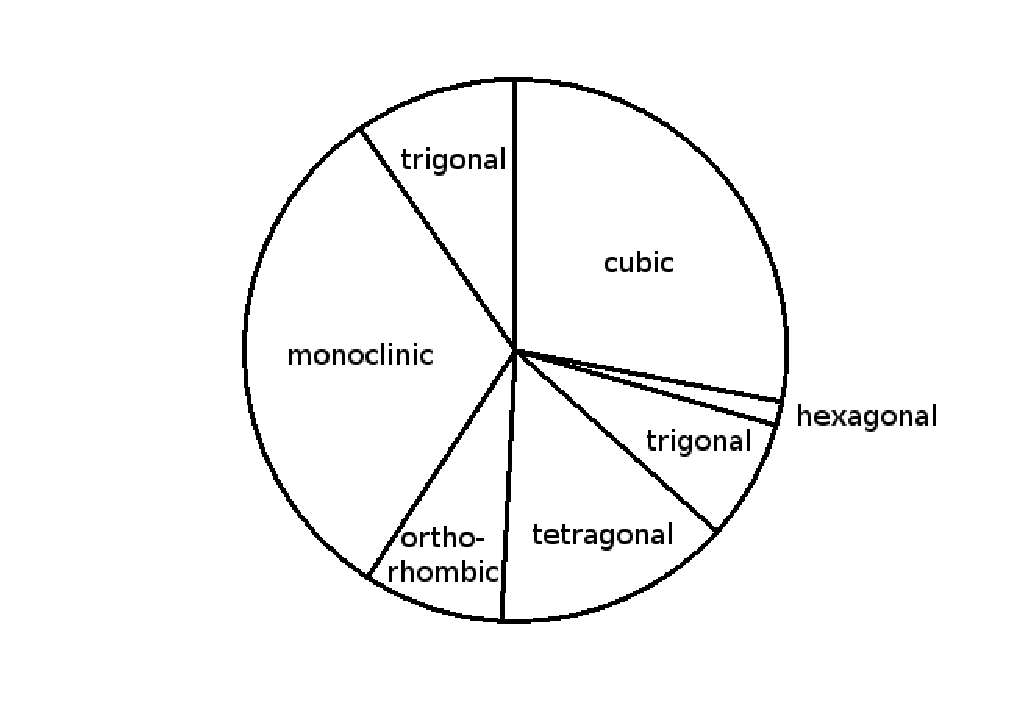
\includegraphics{crystalSystems.eps}
\caption[Crystal structure of tetracarbonyl-nickel in space group
205c]{Crystal structure of tetracarbonyl-nickel [CSD structure
FOJBUB02~\cite{Braga93}] in space group 205c with molecules at
Wyckoff point c. It is a fcc lattice of dimers at Wyckoff point a as
shown for one dimer centered at fractional coordinate
$(1/2,1/2,0)$.\label{dimers}}
\end{center}
\end{figure}

\subsection{Hexagonal and Trigonal Space Groups}

The six structures with hexagonal or trigonal space groups fall
into five structural types summarized in Table~\ref{hex}.  The c/a
ratio is given for the experimental lattice in the third column.
The c/a ratio for the reference lattice is also given.  These are
the ratios of the experimental structure embedded in the reference
lattice. Thus c/a=1.22 for the bcc reference lattice row of the
TCYMET structure entry is not c/a of the bcc crystal but c/a of
TCYMET embedded in the bcc reference lattice. This embedding is
shown in Fig.\ \ref{bccEmbed} in which the lattice constant of the
bcc crystal, $a^\prime$, is compared to the lattice constants a
and c of TCYMET. In each case in Table~\ref{hex} the arbitrary
parameters differ by only a few percent from the ideal reference
lattices. All five reference lattices are sphere packings (hcp,
bcc, or fcc).

\begin{table}
\caption[Reference lattices for hexagonal and trigonal
structures.]{Reference lattices for hexagonal and trigonal
structures. Ideal reference lattice parameters and Wyckoff
structural parameters are listed below the experimental data.}
\label{hex}
\begin{center}
\begin{tabular}{cccccc}%\hline
\cline{1-6}
Structure & Example & c/a & Str.\ Param's & $|G|/Z$ & Entries \\
          & Lattice \\
\cline{1-6}
165d    & DILWIE01  & 3.07  & z=0.122          &  3 & 2 \\
        & hcp       & 3.27  & z=1/8            & 12 \\
161a    & TCYMET    & 1.28  & z=0.000          &  3 & 1 \\
        & bcc       & 1.22  & z=0              & 48 \\
147d    & ZIZHIZ    & 1.51  & z=0.252          &  3 & 1 \\
        & hcp       & 1.63  & z=1/4            & 12 \\
176h    & CUCZUV    & 0.89  & x=0.361, y=0.334 &  2 & 1 \\
        & hcp       & 0.94  & x=1/3, y=1/3     & 12 \\
152b    & MTRETC10  & 2.57  & x=0.715          &  2 & 1 \\
        & fcc       & 2.45  & x=2/3            & 48 \\
\cline{6-6}
\multicolumn{5}{r}{total:} & 6 \\
 \cline{1-6}
\end{tabular}
\end{center}
\end{table}

\begin{figure}
\begin{center}
\scalebox{1}{\includegraphics{tcymetSupercell_2.eps}} \caption[The
crystal structure of TCYMET embedded in a bcc reference
lattice.]{The crystal structure of TCYMET embedded in a bcc
reference lattice. The molecular centers of mass are depicted as spheres. The
lattice constant of the bcc reference lattice, $a^\prime$, is compared to
the lattice constants a and c of TCYMET.\label{bccEmbed}}
\end{center}
\end{figure}

In contrast to the cubic lattices, all of the hexagonal and
trigonal structures in the data set have molecules at Wyckoff
points with variable Wyckoff structural parameters, so their value
is given in the fourth column. Below these are shown the
structural parameters of the reference lattices.  Again the
agreement between the translational arrangements of molecules in a
crystal with a high-symmetry reference lattice is quite good.

\subsection{Tetragonal Space Groups}
\label{sec:tet}

Tetragonal structures are summarized in Table~\ref{tet}. We adopt
the unique c-axis orientation for tetragonal space groups. The ten
structures fall into eight structural types. Structure 142a
contains eight molecular centers in the unit cell.  Their
molecular centers differ by only 1\% from two conventional fcc
cells stacked in the z-direction.  The other structures are less
trivially related to their reference lattices and are tetragonally
distorted to various degrees.

\begin{table}
\caption{Reference lattices for tetragonal structures} \label{tet}
\begin{center}
\begin{tabular}{cccccc}%\hline
\cline{1-6}
Structure & Example & c/a & Str.\ Parameters & $|G|/Z$ & Entries \\
          & Lattice \\
\cline{1-6}
141a    & FUZLUH    & 0.72 & & 8 & 2 \\
        & A5$^\prime$&0.76 & & 8 \\
137b    & FUZTEZ    & 0.70 & & 8 & 1 \\
        & Aa        & 0.82 & & 16 \\
121a    & ZZZKDW01  & 1.49 & & 8 & 1 \\
        & fcc       & 1.41 & & 48 \\
142a    & KUJSIR    & 2.02 & & 4 & 1 \\
        & fcc       & 2.00 & & 48 \\
120c    & YEMRIR    & 1.50 & & 4 & 1 \\
        & sc        & 1.41 & & 48 \\
114a    & ADAMAN08  & 1.34 & & 4 & 2 \\
        & fcc       & 1.41 & & 48 \\
88a     & KANGUB01  & 3.97 & & 4 & 1 \\
        & A5$^{\prime\prime}$& 3.46&&8 \\
88f     & LUFYEQ    & 1.25 & z=0.311&1&1 \\
        & d-Aa$*$     & 1.15 & z=3/8&8 \\
\cline{6-6}
\multicolumn{5}{r}{total:} & 10 \\
\cline{1-6}
\end{tabular} \\
$^*$ dimer packing
\end{center}
\end{table}

With the exception of structure 142a, discussed above, each of the
tetragonal structures is a sub-group of structures 141a, 139a, or
123a. Figure \ref{fig:tetr} gives the neighbor distances for
tetragonal distortions of these lattices.  Note
that there is a tetragonal distortion that transforms fcc and bcc
into one another.  As a result, structures 137b, 121a, 142a, 114a,
and 88f could not be uniquely assigned to a reference lattice
solely based on their group/sub-group relationships.  For these
structures, the $c/a$ ratio provides the requisite additional
information.  The experimental $c/a$ ratios are marked with
circles in Fig.~\ref{fig:tetr}. There appear to be fewer than nine
circles in the figure because several of them overlap. Note that
the experimental structures cluster around the sphere packings
(marked with dashed lines) or distorted lattices with equidistant
neighbors (marked with dotted lines). For instance, the diamond
lattice can be tetragonally distorted to yield six equidistant
second-nearest neighbors (A5$^\prime$ in Fig.\ \ref{fig:tetr} for
$c/a=2/\sqrt{7}$) or eight equidistant nearest neighbors
(A5$^{\prime\prime}$ in Fig.\ \ref{fig:tetr} for $c/a=2\sqrt{3}$). The Aa
reference lattice is a distorted bcc structure and has ten
equidistant nearest neighbors for $c/a=\sqrt{2/3}$. The A6
reference lattice at $c/a=\sqrt{6}$ is a reference lattice for
other molecules discussed in later sections. Also there is an
additional dimer structure, 88f, among them.

\begin{figure}
% \includegraphics{141ab.eps}
% \includegraphics{139ab.eps}
\begin{center}
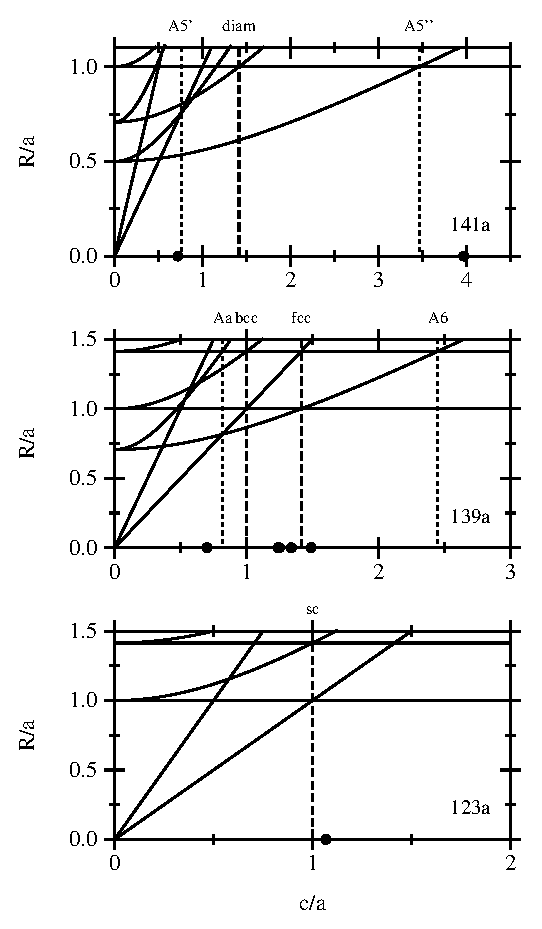
\includegraphics{tetrEPS.eps}
\end{center}
\caption[Neighbor distances for 141a, 139a, and 123a]{Neighbor
distances for 141a, 139a, and 123a as a function of the $c/a$ ratio.
The tetragonal distortions include diam, bcc, fcc, and sc as special
cases.  Experimental values are marked with circles.  Additional
neighbors are omitted for clarity at small $c/a$ values.}
\label{fig:tetr}
\end{figure}

\subsection{Orthorhombic Space Groups}

Orthorhombic structures are summarized in Table~\ref{orth}. We
have adopted the C-centered setting for end centered unit cells.
Each of the six structures constitutes its own distinct structural
type. Two structures, 64d,f and 60c,d very nearly match the fcc
and bcc reference lattices respectively. Structure 19a is
identified with the 63c reference lattice which is an orthorhombic
structure with 10 nearest neighbors and equal c and a lengths. The
b/a=b/c ratio is $\sqrt{5+2\sqrt{6}}$ and the structural parameter
for Wyckoff point c (0,y,1/4) is $y=(\sqrt{6}-1)/4$. The small
discrepancies in the 19a $x$ and $y$ structural parameters in this
case indicate that the molecules have further relaxed from their
reference lattice locations.  The three structures in space group
62 provide additional challenges, discussed below.

\begin{table}
\caption{Reference lattices for orthorhombic structures}
\label{orth}
\begin{center}
\begin{tabular}{ccccccc}%\hline
\cline{1-7}
Structure & Example & b/a & c/a & Str.\ Parameters & $|G|/Z$ & Entries \\
          & Lattice \\
\cline{1-7}
62c     & GUTCED    & 1.10  & 1.09  & x=0.171, z=-0.014   & 2  & 1 \\
        & fcc       & 1.00  & 1.00  & x=1/4, z=0         & 48 \\
62c     & RIMMOP    & 1.46  & 1.61  & x=0.187, z=0.032   & 2  & 1 \\
        & bcc       & 1.41  & 1.41  & x=1/4, z=0         & 48 \\
62c     & JEYSEL    & 1.62  & 1.80  & x=-0.069, z=-0.030   & 2  & 1 \\
        & sh        & 1.63  & 1.73  & x=0, z=0           & 24 \\
64d,f   & METHANEIII& 0.70  & 0.70  & x=0.250            & 1  & 1 \\
        &           &       &       & y=0.230, z=0.270    \\
        & fcc       & 0.71  & 0.71  & x=1/4              & 48 \\
        &           &       &       & y=1/4, z=1/4 \\
19a     & MZNMOX10  & 1.03  & 3.93  & x=-0.066, y=0.067, z=0.123 & 1 & 1 \\
        & 63c       & 1.00  & 3.15  & x=0, y=0, z=0.112          & 4 \\
60c,d   & YIMWEW    & 0.45  & 0.46  & y=-0.188            & 2/3 & 1 \\
        &           &       &       & x=0.169, y=0.297, z=0.206 \\
        & bcc       & 0.47  & 0.47  & y=-1/4              & 48 & \\
        &           &       &       & x=1/6, y=1/4, z=1/4 \\
\cline{7-7}
\multicolumn{6}{r}{total:} & 6 \\
\cline{1-7}
\end{tabular}
\end{center}
\end{table}

Whereas the structures in the data set from the higher crystal
classes are uniquely identified by their space group and Wyckoff
point(s), there are three distinct orthorhombic structures in
space group 62 with molecules at Wyckoff point c.  Therefore, 62c
is insufficient as an identifier for these structures.  Since
there are two arbitrary cell length parameters and two structural
parameters for 62c, it is impractical to plot the neighbor
distances as a function of
arbitrary parameters as in Fig.\ %\ref{fig:205c} and
\ref{fig:tetr}.  Instead we note that Wyckoff point c in space
group 62 has four equivalent positions, two at $y=1/4$ and two at
$y=3/4$. Therefore we view the 3-dimensional structure as a set of
layers in the xz-plane uniformly stacked in the y-direction. Then
the $c/a$ ratio and the structural parameters determine the
symmetry of the layers. CSD structure GUTCED~\cite{Dahl03} is
composed of alternating layers that are nearly on a square
lattice. Based on the stacking of these layers this is a slightly
distorted fcc lattice. CSD structure RIMMOP~\cite{Dahl03} has
alternating rectangular layers, which is more similar to the bcc
reference lattice. The layers in CSD structure JEYSEL are nearly
hexagonal and stacked vertically, rather than alternating.
Therefore, it is associated with the simple hexagonal (sh)
reference lattice.  Thus the three structures in space group 62
are associated with different reference lattices.

\subsection{Monoclinic Space Groups}

Monoclinic structures are shown in Table~\ref{mono}. We adopt the
unique b-axis orientation, cell choice one, origin choice two, and
C centering for end centered lattices. All three lattice
parameters and one lattice angle are able to relax so we indicate
the closeness of the match for b/a, c/a, and $\beta$. The 22
structures fall into 16 distinct structural types. In dividing
into these types it is important to note that monoclinic space
groups have multiple nonstandard settings. Also, during symmetry
breaking from a high-symmetry parent phase to a monoclinic child
phase, multiple domains may form creating unit cells that at first
examination appear to be dissimilar.  An example is CSD structure
REKYUB and CSD structure BOGMEP.  In a standard setting the
important unit cell parameters are
$(b/a,c/a,\beta)=(0.48,1.00,123)$ and $(0.28,0.55,145)$,
respectively. The molecular positions also appear different. However,
these are simply different domains of the same symmetry-breaking
pathway with equivalent unit cell specifications. The phase transition is governed by the same IR, $L_3^-$,
and order parameter direction, P7, using the notation of Stokes
and Hatch~\cite{Stokes02b}. Thus we group them in the same
structural class.

\begin{landscape}
\begin{table}
\caption{Reference lattices for monoclinic structures}
\label{mono}
\begin{center}
\begin{tabular}{cccccccc}%\hline
\cline{1-8}
Structure & Example & b/a & c/a & $\beta$ & Str.\ Parameters & $|G|/Z$ & Entries \\
          & Lattice \\
\cline{1-8}
15e     & REKYUB    & 0.48 & 1.00 & 123 & y=-0.024 & 2 & 3 \\
        & fcc       & 0.58 & 1.16 & 125 & y=0   & 48 \\
15e     & RASDOE    & 0.51 & 0.97 & 120 & y=0.123 & 2 & 1 \\
        & 70a       & 0.50 & 1.00 & 120 & y=1/8   & 4 \\
15e     & TMGEHS10  & 1.78 & 1.14 & 108 & y=0.106 & 2 & 3 \\
        & A5$^\prime$& 1.87 & 1.06 & 118 & y=1/8   & 8 \\
12i     & MECKOU    & 0.73 & 1.17 & 110 & x=0.253, z=0.241 & 2 & 1 \\
        & fcc       & 0.58 & 1.00 & 109 & x=1/4, z=1/4     & 48 \\
11e     & MECKIO    & 1.61 & 1.13 & 105 & x=0.205, y=0.219 & 2 & 1 \\
        & bcc       & 1.63 & 1.00 & 109 & x=1/4, y=1/4     & 48 \\
14e     & TOHSUE    & 1.01 & 2.76 & 90  & x=0.250, y=0.745, z=0.126 & 1 & 1\\
        & fcc       & 1.00 & 2.83 & 90  & x=1/4, y=3/4, z=1/8       & 48 \\
14e     & TMSIAD    & 1.11 & 2.07 & 91  & & 1 & 1 \\
        & d-sh$*$  & 1.22 & 2.12 & 90  & & 12 \\
14e     & CAMPOV    & 1.41 & 1.64 & 92  & & 1 & 2 \\
        & d-sc$*$   & 1.41 & 1.41 & 90  & & 24 \\
14e     & DOCNIS    & 1.45 & 1.80 & 60  & x=0.102, y=0.255, z=0.072 & 1 & 1 \\
        & hcp       & 1.63 & 2.00 & 60  & x=1/6, y=1/4, z=1/12      & 12 \\
14e     & CARBTC    & 0.63 & 1.01 & 104 & x=0.248, y=0.067, z=0.157 & 1 & 1 \\
        & hcp       & 0.61 & 1.06 & 90  & x=1/4, y=0, z=1/6         & 12 \\
14e     & QUGBOJ    & 0.59 & 1.06 & 105 & x=0.268, y=0.129, z=0.070 & 1 & 1\\
        & A5$^\prime$&0.76 & 1.00 & 90  & x=1/4, y=1/8, z=0         & 8 \\
\cline{1-8}
\end{tabular}\\
$^*$ dimer packing
\end{center}
\end{table}
\end{landscape}

\begin{landscape}
\begin{table}
\begin{center}
\begin{tabular}{cccccccc}%\hline
\cline{1-8}
Structure & Example & b/a & c/a & $\beta$ & Str.\ Parameters & $|G|/Z$ & Entries \\
          & Lattice \\
\cline{1-8}
14e     & MECKUA    & 0.66 & 1.14 & 113 & x=0.501, y=0.225, z=0.749 & 1 & 1 \\
        & fcc       & 0.59 & 1.00 & 109 & x=1/2, y=1/4, z=3/4       & 48 \\
14e,e   & CANFIG    & 0.92 & 1.10 & 26  & x=0.331, y=0.340, z=0.005 & 1/2 & 1 \\
        & d-136$*$  & 1.00 & 1.12 & 27  & x=1/3, y=1/3, z=0         & 2 \\
14e,e   & MXSNOX    & 1.76 & 1.74 & 75  & & 1/2 & 1 \\
        & d-sh$*$   & 1.73 & 1.91 & 59  & & 12 \\
13e,f,g & RIMNAC    & 0.52 & 1.84 &  94 & y=0.480 & 1/2 & 1 \\
        &           &      &      &     & y=0.813 \\
        &           &      &      &     & x=0.256, y=0.158, z=0.001 \\
        & 70a       & 0.50 & 1.73 &  90 & y=3/8   & 4 \\
        &           &      &      &     & y=5/8 \\
        &           &      &      &     & x=1/4, y=1/8, z=0 \\
15f,f,f,f  & CTBROM & 0.57 & 0.98 & 111 & x=0.096, y=0.032, z=0.378 & 1/4 & 2 \\
        &           &      &      &     & x=0.379, y=0.060, z=0.120  \\
        &           &      &      &     & x=0.126, y=0.316, z=0.123  \\
        &           &      &      &     & x=0.345, y=0.291, z=0.371  \\
        & fcc       & 0.58 & 1.00 & 109 & x=1/8, y=0, z=3/8          & 48 \\
        &           &      &      &     & x=3/8, y=0, z=1/8  \\
        &           &      &      &     & x=1/8, y=1/4, z=1/8  \\
        &           &      &      &     & x=3/8, y=1/4, z=3/8  \\
\cline{8-8}
\multicolumn{7}{r}{total:} & 22 \\
\cline{1-8}
\end{tabular}\\
$^*$ dimer packing
\end{center}
\end{table}
\end{landscape}

Monoclinic structures have a greater diversity of reference lattices although those
of 9 of the 16 structures are still canonical sphere packings. A
good example of this hidden order in these low-symmetry groups is
15f,f,f,f which has 32 molecules per unit cell and four molecules
per asymmetric unit, but still nearly packs in an fcc lattice.

Many of the structures belong to the same space group but have
different spatial arrangements and so are grouped differently.
This is particularly apparent for space groups 14 and 15, two of
the most populous space groups in the CSD. A5$^\prime$, the
distorted diamond lattice, fits two of the monoclinic structures,
and simple hexagonal two more.  One new packing, 70, is an
orthorhombic distorted diamond lattice and has eight molecules at
Wyckoff point a. The other new packing, 136, is a tetragonal
structure with dimers of molecules at Wyckoff point f. Three additional dimer
structures (TMSIAD, CAMPOV, MXSNOX) have dimers centered at
high symmetry Wykcoff points without structural parameters.

\subsection{Triclinic Space Groups}

Triclinic structures are shown in Table~\ref{tri}. All
lattice parameters are variable and are listed.  The six
structures fall in seven distinct structural types with four
reference lattices. There are two new reference lattices. A6 is a
tetragonal distortion of fcc discussed in Sec.~\ref{sec:tet} and shown
in Fig.~\ref{fig:tetr}. Ai is a rhombohedral distortion intermediate between sc
and bcc. Its primitive cell a, b, and c parameters are all the
same length and $\cos(\alpha)=cos(\beta)=cos(\gamma)=-1/4$. Two
dimer structures in 136 and Ai also exist, the latter with dimer
complexes at a high symmetry Wyckoff point so no structural
parameters are listed in Table~\ref{tri} for XAGXAE.

\begin{landscape}
\begin{table}
\caption{Reference lattices for triclinic structures} \label{tri}
\begin{center}
\begin{tabular}{cccccccccc}%\hline
\cline{1-10}
Structure & Example & b/a & c/a & $\alpha$ & $\beta$ & $\gamma$ & Str.\ Parameters & $|G|/Z$ & Entries \\
          & Lattice \\
\cline{1-10}
2i      & BASXOI    & 1.15 & 1.15 & 86 & 90 & 66 & x=0.297, y=0.306, z=0.299 & 1 & 1 \\
        & A6        & 1.00 & 1.00 & 90 & 90 & 60 & x=1/4, y=1/4, z=1/4       & 16 \\
2i      & XAGXAE    & 1.02 & 1.02 & 93 & 101 & 110 &                         & 1 & 1 \\
        & d-Ai$*$  & 1.15 & 0.83 & 87 & 97 & 116  &                         & 6 \\
2i      & XUWROW    &      &      &    &   &       &                         & & - \\
        & \multicolumn{9}{l}{epitaxial crystal---70\% voids} \\
2i      & MEZDIE01  & 1.46 & 0.92 & 90 & 112 & 90 & x=0.261, y=0.251, z=0.242 & 1 & 2\\
        & bcc       & 1.63 & 1.00 & 90 & 109 & 90 & x=3/4, y=1/4, z=1/4       & 48 \\
2i,i,i  & OHABEE    & 1.49 & 2.57 & 90 & 90 & 90 & x=0.320, y=0.247, z=0.585  & 1/3 & 1 \\
        &           &      &      &    &    &    & x=0.016, y=0.254, z=0.250 \\
        &           &      &      &    &    &    & x=0.318, y=0.754, z=0.082 \\
        & bcc       & 1.63 & 2.83 & 90 & 90 & 90 & x=1/3, y=1/4, z=7/12       & 48 \\
        &           &      &      &    &    &    & x=0, y=1/4, z=1/4 \\
        &           &      &      &    &    &    & x=1/3, y=3/4, z=1/12 \\
2i,i,i,i & CANFOM   & 0.92 & 0.48 & 88 & 91 & 88 & x=0.162, y=0.842, z=0.484  & 1/4 & 1\\
        &           &      &      &    &    &    & x=0.334, y=0.340, z=-0.008 \\
        & d-136$*$  & 1.00 & 0.50 & 90 & 90 & 90 & x=1/6, y=5/6, z=1/2        & 2 \\
        &           &      &      &    &    &    & x=1/3, y=1/3, z=0 \\
\cline{10-10}
\multicolumn{9}{r}{total:} & 7 \\
\cline{1-10}
\end{tabular}\\
$^*$ dimer packing
\end{center}
\end{table}
\end{landscape}

\subsection{Reference Lattice Summary}

The results of the reference lattice assignments of the experimental
structures are summarized in Table~\ref{summary}. The
Strukturbericht designation~\cite{Wilson51}, Pearson
symbol~\cite{Pearson67}, and common name are shown when known for
each reference lattice. The Strukturbericht designations beginning
with an A indicate the reference lattices are also the crystal
structures of various elements. The space group, occupied Wyckoff
positions, and percentage of experimental structures that pertain
to each lattice are also shown.
\begin{landscape}
\begin{table}
\caption{Summary of reference lattices inferred from experimental
data.} \label{summary}\scriptsize
\begin{tabular}{cccccccccc}
\hline
Struktur- & Pearson & Common & Space & Wyckoff & $|G|/Z$ & Comments & Monomer & Dimer & Occurance\\
bericht & Symbol & Name & Group & Point(s) & & & Structures & Structures & Percentage\\
\hline
A2  & cI2 & bcc & 229 & a           & 48 & sphere packing                         & 18 &   & 25.7\%\\
A1  & cF4 & fcc & 225 & a or b      & 48 & sphere packing                         & 15 & 2 & 24.3\%\\
Ah  & cP1 & sc  & 221 & a or b      & 48 & sphere packing                         &  4 & 2 & 8.6\%\\
A3  & hP2 & hcp & 194 & c or d      & 12 & sphere packing                         &  6 &   & 8.6\%\\
A5$^\prime$ & tI4 & & 141 & a or b  &  8 & distorted diamond with c/a=$2/\sqrt 7$ &  6 &   & 8.6\%\\
Af  & hP1 & sh  & 191 & a           & 24 & simple hexagonal                       &  1 & 2 & 4.3\%\\
A15 & cP8 &     & 223 & a and (c or d)&6 & least-area structure                   &  3 &   & 4.3\%\\
Aa  & tI2 & bct & 139 & a or b      & 16 & distorted bcc with c/a=$\sqrt 2/3$    &  1 & 1 & 2.9\%\\
    & tP8 &     & 136 & f,f         &  8 & dimer packing                          &    & 2 & 2.9\%\\
    & oF8 &     & 70  & a           &  4 &                                        &  2 &   & 2.9\%\\
A4  & cF8 & diamond & 227 & a or b  & 24 & sphere packing                         &  1 &   & 1.4\%\\
Ai  & tR2 &     & 166 & a,a         & 18 & dimer packing                          &    & 1 & 1.4\%\\
A6  & tI2 & fct & 139 & a or b      & 16 & distorted fcc with c/a=$\sqrt 6$       &  1 &   & 1.4\%\\
A5$^{\prime\prime}$ & tI4 & & 141 & a or b  & 8 & distorted diamond with c/a=$2\sqrt 3$&1& & 1.4\%\\
    & oC2 &     &  63 & c           &  8 &                                        &  1 &   & 1.4\%\\
\hline
\end{tabular}
\end{table}
\end{landscape}

The fit of each experimental structure to its reference lattice is
summarized in Fig.~\ref{comparison}. In each box the experimental
lattice vectors, angles, or Wyckoff positions are compared with
their idealized values when inscribed in the corresponding reference lattice. These figures
are a visual summary of Tables~\ref{cubic}-\ref{tri}. If the fit
were perfect all data points would lie directly on the line. The fit is quite good
indicating that most low
symmetry molecular crystals have molecules situated at or near lattice
sites of high symmetry space groups. In the inorganic crystal structure database (ICSD), which is largely
composed of atomic crystals,
the most numerous structures are fcc, bcc, hcp, etc.~\cite{Mighell80} Originally this was
considered to be distinct from the CSD which had primarily monoclinic and triclinic structures.
Figure \ref{comparison} challenges this distinction by showing molecular centers of mass,
however, are nearly situated
on lattice points of these archetypical high symmetry lattices
so prevalent in the ICSD. The comparative number of monomer and dimer
structures is shown in Fig.~\ref{dimerMonomer} as is the breakdown
of each into types of reference lattices. It is apparent that
although there are 15 reference lattices, 76\% of the structures
are well represented by only 5 reference lattices.

\begin{figure}
\begin{center}
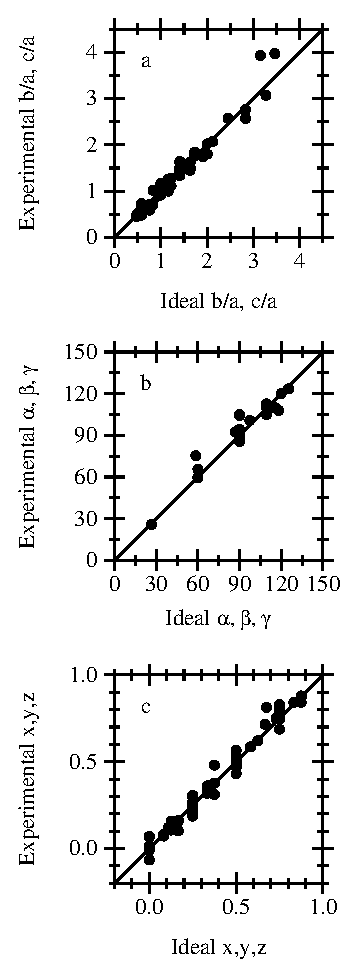
\includegraphics{compare2EPS.eps}
\end{center}
\caption[Comparison of experimental and ideal reference
structures.]{Comparison of experimental and ideal reference (a)
lattice lengths, (b) angles, and (c) structural parameters. The
45-degree line indicates perfect agreement between the experimental
molecular centers and the reference lattice. Scatter around the line
is the result of broken symmetry in orientationally ordered
structures.} \label{comparison}
\end{figure}

\begin{landscape}
\begin{figure}
\begin{center}
\scalebox{.85}{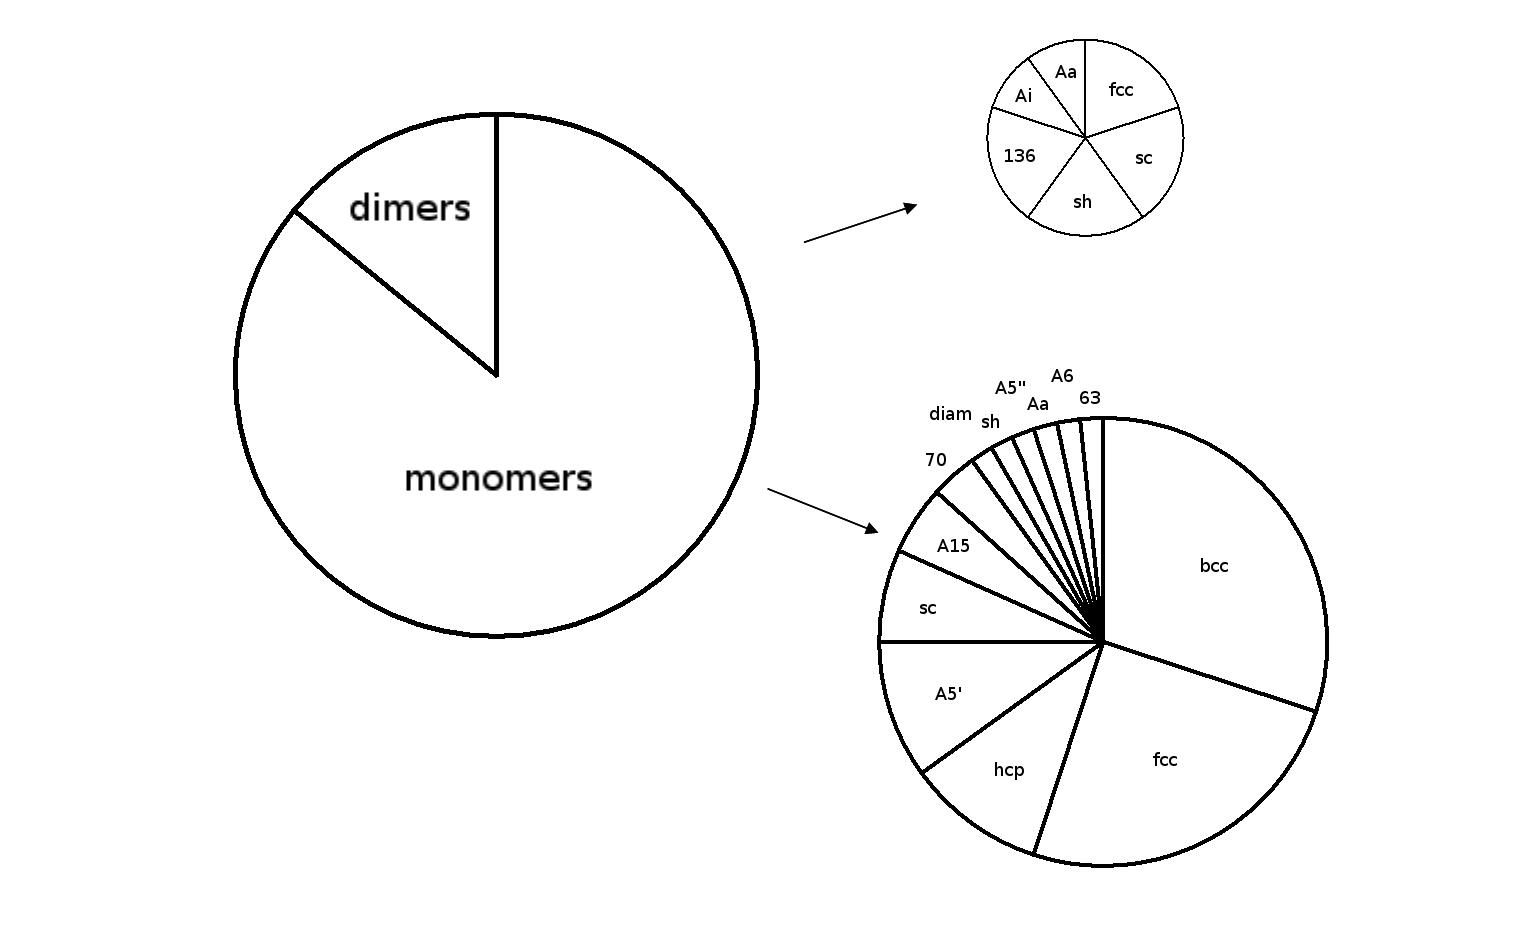
\includegraphics{pieCharts3.eps}}
\end{center}
\caption[Monomer and dimer structures and their reference
lattices.]{Relative proportions of monomer and dimer structures in
the experimental data set and reference lattices
for each.}\label{dimerMonomer}
\end{figure}
\end{landscape}

The dimer structures, reference lattices, and dimer complex point
group symmetries are listed in Table~\ref{tab:dimers}.  Such
structures can usually be identified by examining
nearest neighbor distances. The presence of three or fewer nearest
neighbors is evidence of dimerization. Many of the
structures form $D_{3d}$ or nearly $D_{3d}$ dimers as illustrated
in Fig.~\ref{dimers}, the one exception being CSD structure
LUFYEQ~\cite{Wrackmeyer02} whose molecules form $C_{2v}$
complexes.

\begin{table}
\begin{center}
\caption{Dimer complexes among crystals of tetrahedral
molecules.}\label{tab:dimers}
\begin{tabular}{lccccc}
\hline
structure & dimer & representative & reference & point-group & entries\\
          &Wyck.~Pt.& entry        & lattice   & symmetry \\
\hline
205c & a & FOJBUB02 & d-fcc & $D_{3d}$              & 2\\
88f  & e & LUFYEQ   & d-Aa  & $C_{2v}$              & 1\\
14e  & a & TMSIAD   & d-sh  & $C_i$ ($\sim D_{3d}$) & 1 \\
14e  & a & CAMPOV   & d-sc  & $C_i$ ($\sim D_{3d}$) & 2\\
14e,e& e & CANFIG   & d-136 & $C_1$ ($\sim D_{3d}$) & 1\\
14e,e&b,c& MXSNOX   & d-sh  & $C_i$ ($\sim D_{3d}$) & 1\\
2i   & a & XAGXAE   & d-166 & $D_{3d}$              & 1\\
2i,i,i,i&i,i&CANFOM & d-136 & $C_1$ ($\sim D_{3d}$) & 1 \\
\cline{6-6}
\multicolumn{5}{r}{total:} & 10 \\
\hline
\multicolumn{6}{c}{{\small Note: Point group symmetries
were assigned by visual inspection.}}
\end{tabular}
\end{center}
\end{table}

With the three techniques we have introduced here, (1) dimer
screening by nearest neighbor inspection, (2) reference lattice
assignment by large tolerance molecular center symmetry
determination, (3) reference lattice recognition through template
matching, one may determine translational packings or reference
lattices for all structures in the CSD.  While the second step has
generally been done by hand, the first and third step have been
automated in Python and {M\small ATHEMATICA} scripts and are
available upon request.

\section{Representative Potential Determination}
\label{method}

Global phase diagrams require (1) reference lattices consistent with
molecular centers of mass in experimental structures and (2)
intermolecular potential (IP) parameters to use as independent
parameters. In Sec.~\ref{assignments} we found the majority of the
experimental structures examined can be classified using only five
reference lattices. Since there is little data for other reference
lattices, we focus on the set \{bcc, fcc, hcp, A5$^\prime$, sc\}.
Each of these has at least four monomer crystal structures in the
data set. In this section we seek to determine a \emph{sufficient}
parameter space such that experimental structures are each stable in
a separate subspace. Thus we review our choice of IP and define the
potential parameters.  Then we outline a method for identifying
representative potential parameters for each experimental structure.
This is done using a low temperature structural limit which is
convenient and consistent with with the experimental database but is
not strictly necessary.  Then the IP is truncated to create a finite
dimensional IP parameter space.  A library of alternative crystal
structures is constructed with which to compare experimental
structures, and a figure of merit is specified when searching for
the potential parameters. This procedure identifies a structure with
similar cell shape, molecular center of mass, and molecular
orientations as shown in Fig.~\ref{compare}.

%Having assigned reference lattices for the experimental data set
%in Sec.~\ref{assignments}, we describe a method of reverse
%engineering a representative potential responsible for the observed
%orientational ordering of the molecules on their reference
%lattice. Such a potential would be characteristic of a family of potentials
%consistent with an experimental structure and would be located in a subset of parameter space
%lower in energy than potentials of all other structures.  We expect the size in potential parameter
%space of each family to be rather small due to extreme parameter sensitivity
%is discussed in Refs.~\cite{Keith04c,Mettes04}.

%A comparison of an experimental
%structure with a structure using the potential parameterization we have chosen is shown in Fig.~\ref{compare}. Similar unit cell
%shape and molecular orientation indicates the reference lattice is
%close to the experimental lattice and the rotational ordering is
%similar to the observed molecular orientations. To outline the procedure for obtaining such a potential we
%review the mathematical model and potential
%parameters, discuss a figure of merit for searching parameter
%space, and then describe a computational strategy to optimize the
%parameters.

\begin{figure}
\begin{center}
\scalebox{.5}{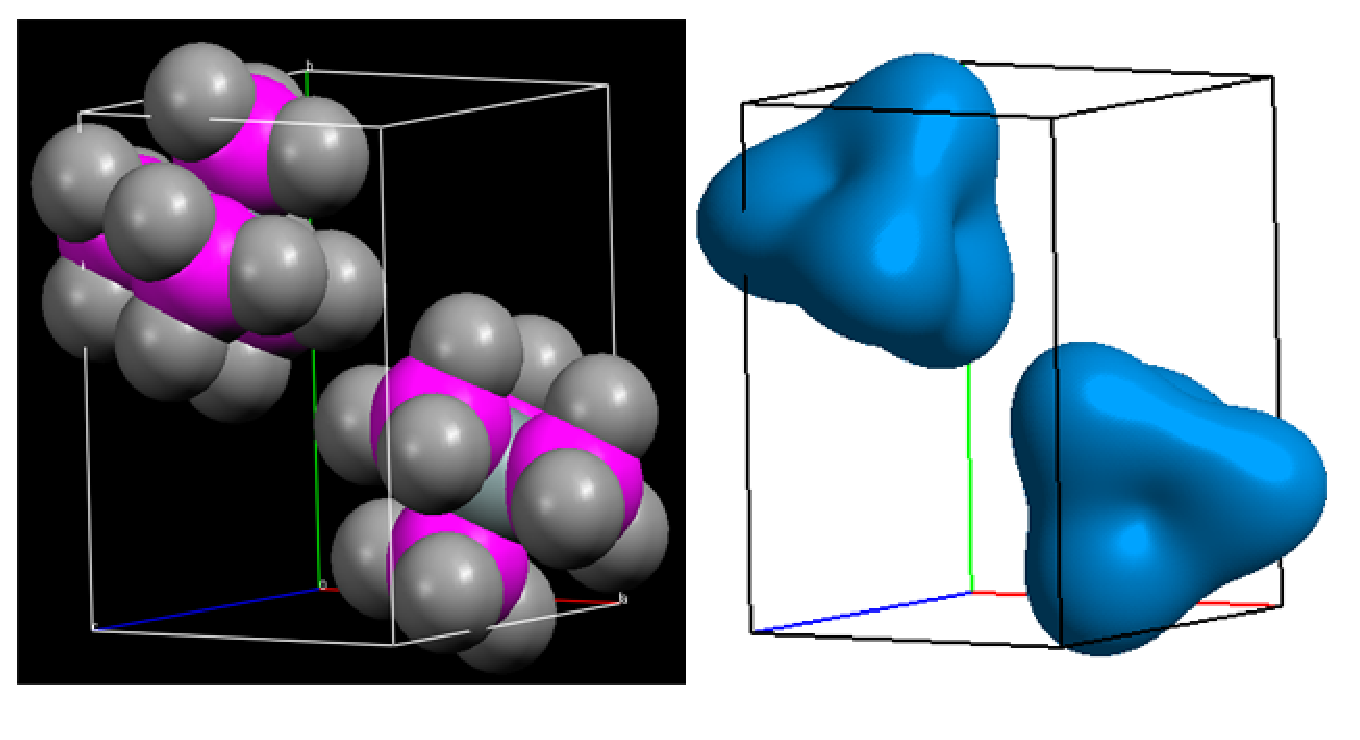
\includegraphics{mezdieCompareII.eps}}
\caption[Comparison of an experimental structure to an an ideal
bcc reference lattice structure.]{Comparison of an experimental
structure, tetrakis(trimethystannyl)silane  [CSD structure
MEZDIE01], which crystallizes in space group 2 at Wyckoff point i
with arbitrarily-shaped tetrahedral figures whose orientation is
determined by orientational energy minimization with molecular
center of mass on an ideal bcc reference lattice.\label{compare}}
\end{center}
\end{figure}

\subsection{Mesoscopic Hamiltonian}
\label{hamiltonian}

Previously~\cite{Mettes04} we discussed the construction of a
nearest neighbor rotational potential for van der Waals molecules.
It is a level of abstraction above an atom-atom or site-site
potential but retains a firm basis in quantum
mechanics~\cite{Avoird94}. The potential consists of a two center expansion constructed by
coupling one center basis functions $U^{\ell_i}_{m_\tau n_\sigma}$
for pairs of molecules $i$ and $j$ and coupling ``matrix"
$J_{m_\tau n_\sigma m_\rho n_\mu}^{\ell_i \ell_j}$,
\begin{equation}
\label{re:eq:vij2}V_{\mathrm{or}} = \frac{1}{2}\sum_{ij}\sum_{\ell_i\ell_j m_\tau m_\rho n_\sigma n_\mu}
U^{\ell_i}_{m_\tau n_\sigma}(\mb{\omega}_i)J_{m_\tau n_\sigma m_\rho n_\mu}^{\ell_i
\ell_j}(\mb{\nu},\mb{\Omega}_{ij})U^{\ell_j}_{m_\rho n_\mu}(\mb{\omega}_i).
\end{equation}
The one half avoids overcounting, $\ell_i,\ell_j\in\mathbb{N}$,
and $|\ell_i-\ell_j|\leq\ell\leq \ell_i+\ell_j$.

$U^{\ell_i}_{m_\tau n_\sigma}(\mb{\omega}_i)$ are functions of
the orientation of the molecule through its Euler angles
$\mb{\omega}_i$ using the passive
convention~\cite{Varshalovich88}.  They are projected from SO(3)
irreducible representations (IR's), also called Wigner functions,
and contain both the point group symmetry of the molecule and that
of the Wyckoff point in the crystal,
\begin{equation}
\label{re:eq:rotfunc}U^{\ell_i}_{m_\tau n_\sigma}(\mb{\omega}_i)=\sum_{m_i n_i}S^{\ell_i*}_{m_im_\tau}D_{m_i
n_i}^{\ell_i}(\mb{\omega}_i)S^{\ell_i}_{n_in_\sigma}.
\end{equation}
The sparse unitary matrix $\mb{S}$ provides the linear
combinations of Wigner functions which give a particular point
group IR symmetry~\cite{Bradley72}.  Specifically, the left
multiplication by $\mb{S}^{-1}$ in Eq.~\ref{re:eq:rotfunc} gives
basis functions transforming like Wyckoff point group IR's and the
right multiplication by $\mb{S}$ gives basis functions of the
molecular point group IR's. Subscript $\tau$ is a compound index
referring to multiple copies of the Wyckoff point group IR
subduced in $\ell_i$ and $m_\tau$ goes over the dimensions of each
IR. Subscript $\sigma$ is a compound index referring to multiple
copies of the molecular point group unit IR subduced in the
$\ell_i$-th manifold of $SO(3)$ and $n_\sigma$ is its dimension.
Point group IR subduction frequencies in spherical harmonics are
discussed elsewhere~\cite{Bradley72} and in
Sec.~\ref{Computational_Strategy}. The symmetry adaption leaves
relatively few basis functions since only matrix elements where
$\sigma$ is the unit IR (\emph{i.e.} $A_1$) are kept.  This gives basis functions in
the molecular frame with the full molecular symmetry.  Thus the
set $\{U^{\ell_i}_{m_\tau n_\sigma}\}$ is a complete set of
functions taking full advantage of symmetry.

The coupling matrix $J_{m_\tau n_\sigma m_\rho n_\mu}^{\ell_i
\ell_j}$ specifies the angular dependence with respect to
molecular centers,
\begin{eqnarray}
\label{coupling} J_{m_\tau n_\sigma m_\rho n_\mu}^{\ell_i
\ell_j}(\mb{\nu},\mb{\Omega}_{ij})&=&\sum_{\ell m_i m m_j}
\nu_{\ell_i,\ell,\ell_j}^{n_\sigma,n_\mu}(r_{ij})\left(\begin{array}{ccc}
 \ell_i & \ell & \ell_j \\ m_i & m & m_j
\end{array}\right)\nonumber\\
&&\times S^{\ell_i}_{m_\tau m_i}C_{m}^{\ell}(\mb{\Omega}_{ij}) S^{\ell_j}_{m_\rho m_j},
\end{eqnarray}
The potential coefficients
$\nu_{\ell_i,\ell,\ell_j}^{n_\sigma,n_\mu}(r_{ij})$ are a function
of the distance $r_{ij}$ between molecular centers. The neighbor
distance $r_{ij}$ and orientation $\Omega_{ij}$ of the
intermolecular vector are determined by the reference lattice.
Since we consider pairwise interactions only among the equidistant
nearest neighbors of the reference lattices, the functions
$\nu_{\ell_i,\ell,\ell_j}^{n_\sigma,n_\mu}(r_{ij})$ are only
evaluated at the nearest neighbor distance and are treated as
scalars. Thus the coupling matrix $J_{m_\tau n_\sigma m_\rho
n_\mu}^{\ell_i \ell_j}$ contains reference lattice information through $\Omega_{ij}$ and $r_{ij}$ as
well as pairwise intermolecular potential information through the coefficients
$\mb{\nu}$. These coefficients have inversion symmetries that
reduce the number of independent values, even for asymmetric
molecules.  In particular
$\nu_{\ell_i,\ell,\ell_j}^{n_\sigma,n_\mu}$ is zero if
$\ell_i+\ell+\ell_j$ is odd and
$\nu_{\ell_i,\ell,\ell_j}^{n_\sigma,n_\mu}=
(-1)^{\ell_i+\ell_j}\nu_{\ell_j,\ell,\ell_i}^{n_\mu,n_\sigma}$ for
single component crystals.~\cite{Avoird80} The full set of
$\nu_{\ell_i,\ell,\ell_j}^{n_\sigma,n_\mu}(r_{ij})$, denoted
$\mb{\nu}$, are the axes of GPD's and the search space for reverse
engineering experimental crystal structures.

\subsection{Computational Strategy}
\label{Computational_Strategy}

Having established translational and rotational components of the
intermolecular potential as the parameter space for GPDs, we seek
to determine potential parameters
$\nu_{\ell_i,\ell,\ell_j}^{n_\sigma,n_\mu}$ sufficient to produce
each experimental crystal structure. Our method has five steps. (1) Define a figure
merit by which to order the crystal structures. (2)
Ensure the potential, Eq.~(\ref{re:eq:vij2}), is truncated such
that it geometrically is able to produce a symmetry change from the assigned reference lattice to the
experimental phase. (3) Develop a library of
structural types against which this energy may be compared. (4)
Determine the energy of an experimental phase as a function of
$\mb{\nu}$. (5) Search potential parameter space until a
$\mb{\nu}$ vector is found which makes the experimental phase
energetically minimal relative to the alternatives in the library.

\subsubsection{Figure of Merit}

In our previous work~\cite{Keith04c,Mettes04} linear response theory was
used to seek phase transitions as a model crystal is cooled from a
disordered plastic crystalline state at high temperature. These transitions are bifurcation points of the free energy surface.
Following each transition, the phase was identified by the
presence of nonzero thermal averages of rotator functions
$U^{\ell_i}_{m_\tau n_\sigma}(\mb{\omega}_i)$ which serve as order
parameters. This work examines the low temperature limit of the
previous model where low is relative to the temperature $T_{pt}$
at which the molecules undergo the first
phase transition from the reference phase. %As the thermal averages
%of the rotator functions are generally quite flat at low
%temperature~\cite{Copley97},
In this regime the function $U^{\ell_i}_{m_\tau n_\sigma}$ itself
is an adequate approximation to the thermal averages of the
rotator functions,
\begin{equation}\label{5a}
\lim_{T/T_{\mathrm{pt}}\rightarrow 0}\av{U^{\ell_i}_{m_\tau n_\sigma}}=U^{\ell_i}_{m_\tau n_\sigma}(\mb{\omega}_0).
\end{equation}
Also, the free energy is equal to the potential in that limit,
\begin{equation}\label{5b}
\lim_{T/T_{\mathrm{pt}}\rightarrow 0}A=V.
\end{equation}
Equations \ref{5a} and \ref{5b} are common approximations used in many
crystal structure prediction codes~\cite{Verwer98} and are further
justified by the exclusion of disordered structures in
\emph{CSDSymmetry} from which our data set is derived.

\subsubsection{Potential Truncation}
\label{truncation}

The potential in Eq.~\ref{re:eq:vij2} is a doubly infinite sum over
manifolds $\ell_i$ and $\ell_j$ that must be truncated for
practical application. To determine an adequate truncation of the
potential we make use of space group irreducible representations (IR's). Symmetry-breaking
mechanisms are classified by space group IR's and an order
parameter direction such as $(a,b)$~\cite{Stokes02b}.  The temperature dependent
values $a$ and $b$ are given in our model by components of space
group IR-adapted basis functions $\mb{q}$ which are linear
combinations of $U^{\ell_i}_{m_\tau
n_\sigma}(\mb{\omega}_i)$~\cite{Mettes04}. Space group IR
distortions of the crystal can be decomposed into point group IR
distortions of the distinguishable molecules in the
crystal~\cite{Stokes91}. To determine which IR's $\tau_w$ of point
group $w$ are in a symmetry-breaking space group IR $\tau_{SG}$,
we calculate their subduction frequencies $n_{SG}$
\begin{eqnarray}
\label{subduction1} n_{SG}=\frac{1}{|w|}\sum_{g\in w}\chi^{\tau_{SG}}(g)^*\chi^{\tau_w}(g)\;\;\;\;\forall\,\,\tau_{SG}
\end{eqnarray}
where $|w|$ is the number of elements $g$ in $w$.
$\chi(g)^{\tau_{SG}}$ and $\chi(g)^{\tau_w}$ are the traces of the
matrix representation of the space group IR and point group IR,
respectively. The calculations are easily performed using the
{I\small SOTROPY} software package~\cite{Stokes02b} using the ``show
frequency'' command. Space group IR and point group IR characters
may also be generated.

Using these point groups one may also
calculate the number of times each point group IR $\tau_w$ appears for each manifold of SO(3), or $\ell_i$ value,
\begin{eqnarray}
\label{subduction2} n_{SO(3)}=\frac{1}{|w|}\sum_{g\in w}\chi^{\ell_i}(g)^*\chi^{\tau_w}(g)\;\;\;\;\forall\,\,\ell_i
\end{eqnarray}
where $\chi^{\ell_i}$ is the trace of the matrix representation of
an IR of SO(3) also called a Wigner rotation matrix. Such subduction frequencies may be easily calculated but are most accesible in standard tables in the literature~\cite{Bradley72} and are shown for $O_h$ and $D_{3h}$ in
Table~\ref{wyckoff_IRs}.  As there is no molecular unit IR in the
first, second, or fifth manifold, there are no Wyckoff IR rows of
$U^{\ell_i}_{m_\tau n_\sigma}$ so these manifolds are not shown.

\begin{table}
\begin{center}
\caption[Presence of $O_h$ and $D_{3h}$ point group IR's for
various manifolds of SO(3).]{Presence of $O_h$ and $D_{3h}$ point
group IR's for various manifolds of SO(3). $O_h$ is the Wyckoff
point group of the fcc, bcc, and sc reference lattices. $D_{3h}$
is the Wyckoff point group of the hcp reference lattice. The first
occurrence of a given IR is shown in bold.}\label{wyckoff_IRs}
\begin{tabular}{lll}\hline
$\ell_i$ & $O_h$ IR's &  $D_{3h}$ IR's\\
\hline
3 & $\mb{A_{2u}}+\mb{T_{1u}}+\mb{T_{2u}}$ & $\mb{A^\prime_1}+\mb{A^{\prime}_2}+\mb{E^\prime}+\mb{E^{\prime\prime}}$ \\
4 & $\mb{A_{1g}}+\mb{E_{g}}+\mb{T_{1g}}+\mb{T_{2g}}$ & $A^\prime_1+\mb{A^{\prime\prime}_1}+\mb{A^{\prime\prime}_2}+2E^\prime+E^{\prime\prime}$ \\
6 & $A_{1g}+\mb{A_{2g}}+E_g+T_{1g}+2T_{2g}$ & $2A^\prime_1+A^{\prime\prime}_1+A^{\prime}_2+A^{\prime\prime}_2+2E^\prime+2E^{\prime\prime}$\\
7 & $A_{2u}+\mb{E_u}+2T_{1u}+2T_{2u}$ & $A^\prime_1+A^{\prime\prime}_1+A^{\prime}_2+2A^{\prime\prime}_2+3E^\prime+2E^{\prime\prime}$ \\
8 & $A_{1g}+2E_g+2T_{1g}+2T_{2g}$ & \\
9 & $\mb{A_{1u}}+A_{2u}+E_u+3T_{1u}+2T_{2u}$ & \\
\hline
\end{tabular}
\end{center}
\end{table}

If the potential is truncated before the manifold at which a Wyckoff
IR forming a symmetry-breaking space group IR is present
(\emph{i.e.} if $n_{SG}=0$ in Eq.\ \ref{subduction1}), the desired
phase transition cannot occur with that potential. Therefore we
calculate minimal SO(3) manifolds necessary to achieve a transition
from the assigned reference lattice to an experimental structure.
This is shown for the reference lattice set \{bcc, fcc, hcp,
A5$^\prime$, sc\} in Tables~\ref{pathwaysBCC}-\ref{pathwaysSC}.
Point group IR's subduced in the space group IR and the first
manifold or $\ell_i$ value of SO(3) at which a given Wyckoff IR
appears are also shown. For some pathways, such as 221a
$\rightarrow$ 215a in Table~\ref{pathwaysSC}, there is a single
space group IR $\Gamma_2^-$ subducing a single point group IR
$A_{2u}$. Table~\ref{wyckoff_IRs} shows that this point group IR
first occurs in the third manifold of SO(3) when split by an $O_h$
point group crystal field.  Thus $\ell_i^{\mathrm{max}}\geq 3$ may
give the 215a structure. For other pathways, such as 194c
$\rightarrow$ 165d in Table~\ref{pathwaysHCP}, there is more than
one Wyckoff IR subduced in a space group IR. Both $A^\prime_1$ and
$A^\prime_2$ can lead to this transition and both are present at the
third manifold (Table~\ref{wyckoff_IRs}). For still others, such as
194c $\rightarrow$ 147d in Table~\ref{pathwaysHCP}, the pathway is
coupled, or composed of the direct sum of two space group IR's.
Three different coupled space group IR's decompose into three
different point group IR's. One of these pathways uses IR's on the
third manifold of SO(3) ($\ell^{\mathrm{max}}_i\geq 3$) while the
other two require fourth manifold basis functions.
Tables~\ref{pathwaysBCC}-\ref{pathwaysSC} show symmetry-breaking
Wyckoff IR's appear by at least the third or fourth manifold in
nearly all cases and at worst at the ninth manifold only for the
$A_{1u}$ IR of the $O_h$ Wyckoff point group.

\begin{table}
\begin{center}
\caption[Group theoretical symmetry-breaking pathways of
experimental lattices for the bcc reference lattice.]{Group theoretical
symmetry-breaking pathways of experimental lattices from the
bcc reference lattice. Classified by space group IR and order
parameter direction, each pathway shows the point group IR and
minimal manifold of SO(3) in Eq.~(\ref{re:eq:vij2}) required to
achieve it.  The order parameter directions are given in the
notation of Stokes and
Hatch~\cite{Stokes02a}.}\label{pathwaysBCC} \footnotesize
\begin{tabular}{lllll}\hline
Pathway & S.~G.~IR & OP Dir. & P.~G.~IR & $\ell^{\mathrm{req'd}}$  \\
\hline
229a $\rightarrow$ 217a & $\Gamma_2^-$ & P1 & $A_{2u}$ & 3 \\

229a $\rightarrow$ 161a & $H_5^- \oplus \Gamma_2^-$ & P3 $\oplus$ P1 & $T_{2u} \oplus
A_{2u}$ & 3 \\
& $H_5^- \oplus \Gamma_4^-$ & P3 $\oplus$ P3 & $T_{2u} \oplus
T_{1u}$ &3 \\
& $H_5^- \oplus H_4^+$ & P3 $\oplus$ P3 & $T_{2u} \oplus T_{1g}$
& 4 \\
& $H_4^+ \oplus \Gamma_2^-$ & P3 $\oplus$ P1 & $T_{1g} \oplus A_{2u}$ & 4 \\
& $H_4^+ \oplus \Gamma_4^-$ & P3 $\oplus$ P3 & $T_{1g} \oplus T_{1u}$ & 4\\
& $H_5^- \oplus H_2^+$ & P3 $\oplus$ P1 & $T_{2u} \oplus A_{2g}$
& 6\\
& $H_2^+ \oplus \Gamma_4^-$ & P1 $\oplus$ P3 & $A_{2g} \oplus T_{1u}$ & 6 \\
& $H_1^- \oplus \Gamma_4^-$ & P1 $\oplus$ P3 & $A_{1u} \oplus
T_{1u}$ & 9 \\
& $H_1^- \oplus H_4^+$ & P1 $\oplus$ P3 & $A_{1u} \oplus T_{1g}$
& 9\\

229a $\rightarrow$ 62c (RIMMOP) & $N_2^- \oplus N_4^+$ & P1
$\oplus$ P1 & $A_{2u},E_u,T_{1u} \oplus T_{1g},T_{2g}$ & 4 \\

229a $\rightarrow$ 60c,d (YIMWEW) & $^*$\\

229a $\rightarrow$ 11e & $N_4^- \oplus N_2^-$ & P1 $\oplus$ P1 & $T_{1u},T_{2u} \oplus
A_{2u},E_u,T_{1u}$ & 3\\
&  & P1 $\oplus$ C1  \\
& $N_2^- \oplus \Gamma_4^+$ & P1
$\oplus$ P2 & $A_{2u},E_u,T_{1u} \oplus T_{1g}$ & 4\\
&  & C1 $\oplus$ P2 \\
& $N_2^- \oplus \Gamma_5^+$ & P1 $\oplus$ C2 & $A_{2u},E_u,T_{1u}
\oplus T_{2g}$ & 4 \\
& & C1 $\oplus$ C2 \\
& $N_4^- \oplus \Gamma_4^+$ & P1 $\oplus$ P2 & $T_{1u},T_{2u}
\oplus T_{1g}$ & 4 \\
& $N_4^- \oplus \Gamma_5^+$ & P1 $\oplus$ C2 & $T_{1u},T_{2u}
\oplus T_{2g}$ & 4 \\

229a $\rightarrow$ 2i (MEZDIE01) & $N_1^-\oplus\Gamma_4^+$ &
P1 $\oplus$ S1 & $A_{1u},E_u,T_{2u} \oplus T_{1g}$ & 4\\
& $N_1^-\oplus\Gamma_5^+$ & P1 $\oplus$ S1 & $A_{1u},E_u,T_{2u}
\oplus T_{2g}$ & 4\\
& $N_2^-\oplus\Gamma_4^+$ & P1 $\oplus$ S1 & $A_{2u},E_u,T_{1u}
\oplus T_{1g}$ & 4 \\
& $N_2^-\oplus\Gamma_5^+$ & P1 $\oplus$ S1 & $A_{2u},E_u,T_{1u}
\oplus T_{2g}$ & 4 \\
& $N_3^-\oplus\Gamma_4^+$ & P1 $\oplus$ S1 & $T_{1u},T_{2u} \oplus
T_{1g}$ & 4\\
& $N_3^-\oplus\Gamma_5^+$ & P1 $\oplus$ S1 & $T_{1u},T_{2u} \oplus
T_{2g}$ & 4\\
& $N_4^-\oplus\Gamma_4^+$ & P1 $\oplus$ S1 & $T_{1u},T_{2u} \oplus
T_{1g}$ & 4\\
& $N_4^-\oplus\Gamma_5^+$ & P1 $\oplus$ S1 & $T_{1u},T_{2u} \oplus
T_{2g}$ & 4\\

229a $\rightarrow$ 2iii & $H_4^-$ & S1 & $T_{1u}$ & 3\\
& H5- & S1 & $T_{2u}$ & 3\\
\hline \multicolumn{5}{c}{$^*$The IR leading to this phase
transition is
a coupled IR between a high symmetry point}\\
\multicolumn{5}{c}{and line which ISOTROPY currently
cannot handle so it is not listed.}
\end{tabular}
\end{center}
\end{table}

\begin{table}
\begin{center}
\caption[Group theoretical symmetry-breaking pathways of
experimental lattices for the fcc reference lattice.]{Group
theoretical symmetry-breaking pathways of experimental lattices
for the fcc reference lattice.} \label{pathwaysFCC}\scriptsize
\begin{tabular}{lllll}\hline
Pathway & S.~G.~IR & OP Dir. & P.~G.~IR & $\ell^{\mathrm{req'd}}$  \\
\hline
225a $\rightarrow$ 152b & $\Lambda_3$ (k=1/3) &  P1 & $E_g,T_{1g},T_{2g},E_u,T_{1u},T_{2u}$ & 3 \\
225a $\rightarrow$ 142a & $W_3$ & P2 & $T_{1g},A_{2u},E_{u}$ & 3 \\

225a $\rightarrow$ 121a & $\Gamma_5^-$ & P1 & $T_{2u}$ & 3 \\

225a $\rightarrow$ 114a & $X_2^-\oplus \Gamma_5^-$ & P1 $\oplus$ P1 & $A_{2u},E_u \oplus
T_{2u}$ & 3 \\
& $X_3^+\oplus \Gamma_5^-$ &
P1 $\oplus$ P1 & $T_{1g} \oplus T_{2u}$ & 4 \\
& $X_2^- \oplus X_3^+$ & P1 $\oplus$ P1 & $A_{2u},E_{u} \oplus
T_{1g}$ & 4 \\

225a $\rightarrow$ 64d,f & $^*$\\

225a $\rightarrow$ 62c & $X_5^-$ & C11 & $T_{1u},T_{2u}$ & 3 \\

225a $\rightarrow$ 15f,f,f,f & $C_2$ ($k_1=1/4,k_2=3/4$) & C18,C19 & $A_{2g},E_g,T_{1g},T_{2g},$ & 3 \\
&  & & $A_{1u},E_u,T_{1u},T_{2u}$\\
%225a $\rightarrow$ 15e (Rasdoe) & L_3^- & P7 & $E_u,T_{1u},T_{2u} & 3 \\

225a $\rightarrow$ 15e (REKYUB) & $L_3^-$ & P7 &
$E_u,T_{1u},T_{2u}$ & 3 \\

225a $\rightarrow$ 14e (MECKUA) & $\Gamma_3^+ \oplus L_3^-$ & P1 $\oplus$ C8 & $E_g \oplus E_u,T_{1u},T_{2u}$ & 4 \\
& $\Gamma_3^+ \oplus X_5^-$ & C1 $\oplus$ S7 & $E_g \oplus T_{1u},T_{2u}$ & 4 \\
& $\Gamma_4^+ \oplus X_5^-$ & P1 $\oplus$ C11  & $T_{1g} \oplus T_{1u},T_{2u}$ & 4 \\
& & P1 $\oplus$ S7 \\
& $\Gamma_5^+ \oplus L_3^-$ & C2 $\oplus$ C8 & $T_{2g} \oplus E_u,T_{1u},T_{2u}$ & 4 \\
& $\Gamma_5^+ \oplus X_5^-$ & P1 $\oplus$ C11 & $T_{2g} \oplus T_{1u},T_{2u}$ & 4 \\
& & P1 $\oplus$ S7 & &  \\
& $L_2^+ \oplus L_1^-$ & P1 $\oplus$ P1 & $A_{2g},T_{1g} \oplus A_{1u},T_{2u}$ & 4 \\

& $L_2^+ \oplus L_3^-$ &  P1 $\oplus$ P7 & $A_{2g},T_{1g} \oplus E_u,T_{1u},T_{2u}$ & 4 \\

& $L_2^+ \oplus X_2^-$ &  P1 $\oplus$ P1 & $A_{2g},T_{1g} \oplus A_{2u},E_u$ & 4 \\

& $L_2^+ \oplus X_3^-$ &  P1 $\oplus$ P1 & $A_{2g},T_{1g} \oplus E_u,T_{1u}$ & 4 \\

& $L_2^+ \oplus X_5^-$ &  P1 $\oplus$ P1 & $A_{2g},T_{1g} \oplus T_{1u},T_{2u}$ & 4 \\

& $L_3^+ \oplus L_1^-$ &  P7 $\oplus$ P1 & $E_g,T_{1g},T_{2g} \oplus A_{1u},T_{2u}$ & 4 \\

& $L_3^+ \oplus L_3^-$ &  P7 $\oplus$ P7 & $E_g,T_{1g},T_{2g} \oplus E_u,T_{1u},T_{2u}$ & 4 \\

& $L_3^+ \oplus X_2^-$ &  P7 $\oplus$ P1 & $E_g,T_{1g},T_{2g} \oplus A_{2u},E_u$ & 4 \\

& $L_3^+ \oplus X_3^-$ &  P7 $\oplus$ P1 & $E_g,T_{1g},T_{2g} \oplus E_u,T_{1u}$ & 4 \\

& $L_3^+ \oplus X_5^-$ &  P7 $\oplus$ P1 & $E_g,T_{1g},T_{2g} \oplus T_{1u},T_{2u}$ & 4 \\

& $L_1^- \oplus L_3^-$ &  P1 $\oplus$ C8 & $A_{1u},T_{2u} \oplus E_u,T_{1u},T_{2u}$ & 4 \\

& $L_1^- \oplus X_2^-$ &  P1 $\oplus$ P1 & $A_{1u},T_{2u} \oplus A_{2u},E_u$ & 4 \\

& $L_1^- \oplus X_3^-$ &  P1 $\oplus$ P1 & $A_{1u},T_{2u} \oplus E_u,T_{1u}$ & 4 \\

& $L_1^- \oplus X_5^-$ &  P1 $\oplus$ P1 & $A_{1u},T_{2u} \oplus T_{1u},T_{2u}$ & 4 \\

& $L_3^- \oplus X_2^-$ &  P7 $\oplus$ P1 & $E_u,T_{1u},T_{2u} \oplus A_{2u},E_u$ & 4 \\

& $L_3^- \oplus X_3^-$ &  P7 $\oplus$ P1 & $E_u,T_{1u},T_{2u} \oplus E_u,T_{1u}$ & 4 \\

& $L_3^- \oplus X_5^-$ &  P7 $\oplus$ P1 & $E_u,T_{1u},T_{2u} \oplus T_{1u},T_{2u}$ & 4 \\

& $X_2^- \oplus X_5^-$ &  P1 $\oplus$ C11 & $A_{2u},E_u \oplus T_{1u},T_{2u}$ & 4 \\

& & P1 $\oplus$ S7 & &  \\

& $X_3^- \oplus X_5^-$ &  P1 $\oplus$ C11 & $E_u,T_{1u} \oplus T_{1u},T_{2u}$ & 4 \\

225a $\rightarrow$ 14e (TOHSUE) & $\Delta_5$ ($k=1/4$) & C7 &
$T_{1g},T_{2g},T_{1u},T_{2u}$ & 3 \\

225a $\rightarrow$ 12i & $L_3^-$ & P2 & $E_u,T_{1u},T_{2u}$ & 3 \\

225a $\rightarrow$ 11e & $X_5^-$ & C1 & $T_{1u},T_{2u}$ & 3\\
\hline \multicolumn{5}{c}{$^*$The IR leading to this phase
transition is
a coupled IR between a high symmetry point}\\
\multicolumn{5}{c}{and line which ISOTROPY currently
cannot handle so it is not listed.}
\end{tabular}
\end{center}
\end{table}

\begin{table}
\begin{center}
\caption[Group theoretical symmetry-breaking pathways of
experimental lattices from hcp.]{Group theoretical
symmetry-breaking pathways of experimental lattices for the hcp
reference lattice.}\label{pathwaysHCP}\footnotesize
\begin{tabular}{lllll}\hline
Pathway & S.~G.~IR & OP Dir. & P.~G.~IR & $\ell^{\mathrm{req'd}}$ \\
\hline
194c $\rightarrow$ 176h & $K_4$ & (a,0) & $E^\prime$ & 3 \\
194c $\rightarrow$ 165d & $A_2$ & (a,a) & $A_2^\prime,A_1^\prime$ & 3 \\
194c $\rightarrow$ 147d & $\Gamma_3^+ \oplus \Gamma_2^+$ & (a,b) & $A_2^{\prime\prime}\oplus A_2^\prime$ & 3 \\
& $\Gamma_4^+ \oplus \Gamma_2^+$ & (a,b) & $A_1^{\prime\prime}\oplus A_2^\prime$ & 4 \\
& $\Gamma_4^+ \oplus \Gamma_3^+$ & (a,b) & $A_1^{\prime\prime}\oplus A_2^{\prime\prime}$ & 4 \\
194c  $\rightarrow$ 14e DOCNIS & $M_1^-\oplus \Gamma_2^+$ & (a,0,0,b) & $A_1^{\prime\prime},E^{\prime\prime} \oplus A_2^\prime $ & 3 \\
& $M_1^- \oplus \Gamma_2^+$ & (a,b,0,c) & $A_1^{\prime\prime},E^{\prime\prime} \oplus A_2^\prime$ & 3 \\
& $M_1^- \oplus \Gamma_5^+$ & (a,0,0,b,c) & $A_1^{\prime\prime},E^{\prime\prime} \oplus E^{\prime}$ & 3 \\
& $M_1^- \oplus \Gamma_5^+$ & (a,b,0,c,d) & $A_1^{\prime\prime},E^{\prime\prime} \oplus E^\prime$ & 3 \\
& $M_2^- \oplus \Gamma_2^+$ & (a,0,0,b) & $A_2^{\prime\prime},E^{\prime\prime} \oplus A_2^\prime$ & 3 \\
& $M_2^- \oplus \Gamma_2^+$ & (a,b,0,c) & $A_2^{\prime\prime},E^{\prime\prime} \oplus A_2^\prime$ & 3 \\
& $M_2^- \oplus \Gamma_5^+$ & (a,0,0,b,c) & $A_2^{\prime\prime},E^{\prime\prime} \oplus E^\prime$ & 3 \\
& $M_2^- \oplus \Gamma_5^+$ & (a,b,0,c,d) & $A_2^{\prime\prime},E^{\prime\prime} \oplus E^\prime$ & 3 \\
& $M_2^- \oplus M_1^- $ & (a,0,0,b,0,0) & $A_2^{\prime\prime},E^{\prime\prime} \oplus A_1^{\prime\prime},E^{\prime\prime}$ & 3 \\
& $M_2^- \oplus M_1^-$ & (a,b,0,c,d,0) & $A_2^{\prime\prime},E^{\prime\prime} \oplus A_1^{\prime\prime},E^{\prime\prime}$ & 3 \\
194c  $\rightarrow$ 14e CARBTC & $M_2^+ \oplus \Gamma_6^+$ & (a,0,0,0,b) &  $A_2^\prime,E^\prime \oplus E^{\prime\prime}$ & 3 \\
& $M_2^+ \oplus \Gamma_6^+$ & (a,0,0,b,0)  &  $A_2^\prime,E^\prime \oplus E^{\prime\prime}$ & 3 \\
& $M_2^+ \oplus \Gamma_3^+$ & (a,0,0,b) &  $A_2^\prime,E^\prime \oplus A_2^{\prime\prime}$ & 4 \\
& $M_4^+ \oplus \Gamma_3^+$ & (a,0,0,b) &   $A_1^{\prime\prime},E^{\prime\prime} \oplus A_2^{\prime\prime}$ & 4 \\
& $M_4^+ \oplus \Gamma_5^+$ & (a,0,0,b,c) &  $A_1^{\prime\prime},E^{\prime\prime} \oplus E^\prime$ & 4 \\
& $M_4^+ \oplus \Gamma_6^+$ & (a,0,0,0,b) &  $A_1^{\prime\prime},E^{\prime\prime} \oplus E^{\prime\prime}$ & 4 \\
& $M_4^+ \oplus M_2^+$  & (a,0,0,b,0,0) & $A_1^{\prime\prime},E^{\prime\prime} \oplus A_2^\prime,E^\prime$ & 4 \\
\hline
\end{tabular}
\end{center}
\end{table}

\begin{table}
\begin{center}
\caption[Group theoretical symmetry-breaking pathways of
experimental lattices for the A5$^\prime$ reference lattice.]{Group
theoretical symmetry-breaking pathways of experimental lattices
for the A5$^\prime$ reference lattice.} \label{pathwaysA5}
\begin{tabular}{lllll}\hline
Pathway & S.~G.~IR & OP Dir. & P.~G.~IR & $\ell^{\mathrm{req'd}}$  \\
\hline
A5 $\rightarrow$ 141a & $\Gamma_1^+$ &  P1 & $A_{1}$ & 3 \\
A5 $\rightarrow$ 15e & $\Gamma_5^+$ &  P3 & $E$ & 3 \\
A5 $\rightarrow$ 14e & $\Gamma_3^+ \oplus M_3 $ &  P1 $\oplus$ P3 & $A_{2} \oplus E $ & 3 \\
& $\Gamma_3^+ \oplus M_4 $ &  P1 $\oplus$ P3 & $A_{2} \oplus E$ &  3\\
& $M_3 \oplus M_4 $ &  P3 $\oplus$ P3 & $E \oplus E$ &  3\\
&  $\Gamma_4^+ \oplus M_3 $ &  P1 $\oplus$ P3 & $B_{1} \oplus E$ &  4\\
& $\Gamma_4^+ \oplus M_4 $ &  P1 $\oplus$ P3 & $B_{1} \oplus E$ &  4\\
\hline
\end{tabular}
\end{center}
\end{table}

\begin{table}
\begin{center}
\caption[Group theoretical symmetry-breaking pathways of
experimental lattices from sc.]{Group theoretical
symmetry-breaking pathways of experimental lattices for
the sc reference lattice.}\label{pathwaysSC}\footnotesize
\begin{tabular}{lllll}\hline
Pathway & S.~G.~IR & OP Dir. & P.~G.~IR & $\ell^{\mathrm{req'd}}$  \\
\hline
221a $\rightarrow$ 215a & $\Gamma_2^-$ & (a) & $A_{2u}$ & 3 \\
221a $\rightarrow$ 120c & $R_5^-\oplus \Gamma_2^-$ & (a,0,0,b) & $T_{2u} \oplus A_{2u}$  & 3 \\
& $R_4^+\oplus \Gamma_2^-$ & (a,0,0,b) & $T_{1g} \oplus A_{2u}$ & 4 \\
& $R_5^-\oplus R_4^+$ & (a,0,0,b,0,0) & $T_{2u} \oplus T_{1g}$  & 4 \\
& $R_4^+\oplus \Gamma_3^-$ & (a,0,0,b,0) & $T_{1g} \oplus E_u$  & 7 \\
& $R_5^-\oplus \Gamma_3^-$ & (a,0,0,b,0) & $T_{2u} \oplus E_u$  & 7 \\
\hline
\end{tabular}
\end{center}
\end{table}

In real phase transitions, IR's on the first non-trivial manifold
typically induce symmetry breaking. Second manifold induced
symmetry breaking is uncommon and higher manifold induced phase
transitions are not generally observed.~\cite{LyndenBell94} The
reasons for this are different for small and large molecules. For small molecules with only a few
atoms (\emph{i.e.} CH$_4$) molecular orbitals
tend to form low-energy, slowly varying topologies to lessen
kinetic energy contributions in Schr\"{o}dinger's equation. The result is an
IP well represented by smooth, slowly varying basis functions. For large
molecules, low manifold contributions to the potential are
sufficient to locate attractive/repulsive regions of the potential
and the relative magnitudes of attractive configurations, even
though these basis functions are not sufficient to represent the
fine structure in the potential due to individual atoms.~\cite{Hloucha01}
In either case, the most important aspects of the IP are given by slowly varying
functions  while more rapidly varying functions produce finer details. Thus as a
minimal basis set we truncate Eq.~\ref{re:eq:vij2} at
$\ell_{\mathrm{max}}=3$ or 4.

Truncating at $\ell_\mathrm{max}=4$ leaves fifteen coefficients in
the potential, $\nu_{0,3,3}$, $\nu_{0,4,4}$, $\nu_{3,0,3}$,
$\nu_{3,2,3}$, $\nu_{3,4,3}$, $\nu_{3,6,3}$, $\nu_{3,1,4}$,
$\nu_{3,3,4}$, $\nu_{3,5,4}$, $\nu_{3,7,4}$, $\nu_{4,0,4}$,
$\nu_{4,2,4}$, $\nu_{4,4,4}$, $\nu_{4,6,4}$, and $\nu_{4,8,4}$.
The coefficient $\nu_{0,0,0}$ is negligible since it only affects the trivial basis function
$U_{0,0}^0=1$ which is isotropic and therefore unimportant in
rotational ordering.  As the unit IR for $T_d$ appears \emph{once}
in the zeroth, third and fourth manifolds, $n_\sigma$ and $n_\mu$
are always $1_{A_1}$ and have been dropped in the notation
for the coefficients in Eq.~\ref{coupling}. For space groups whose
occupied Wyckoff point group in the reference lattice has the
inversion as one of its symmetry operators, $\nu_{0,x,x}$ cancels
in the crystal field for odd values of $x$. This is the case with the $\nu_{033}$ coefficient in the
bcc, fcc, and sc reference lattices with 14 coefficients but not for hcp or A5$^\prime$ with
15.

\subsubsection{Candidate Lattice Library}
\label{collection}

We seek a set of potential parameters $\mb{\nu}$ such that the energy is lower than
other structures, whether observed or not. Therefore, a comparative
list of structural types should consist of both the
experimental structures and a large library of alternate
structures. Each alternative structure serves to constrain the representative potential
parameters \mb{\nu} identified with each
experimental structure.  In our previous
work~\cite{Mettes04}, high symmetry point IR
distortions~\cite{Stokes88,Stokes02b} from a reference lattice led
to structures classified using their isotropy subgroups (ISs).
These subgroups represent the most common types of phase transitions and are minimal
in the sense that only one domain of each structure is tested.
This compares favorably to crystal structure prediction which generates
thousands of multi-domain duplicate structures.  Therefore they are convenient
for constructing a library of candidate lattices. They are discussed further in
Sec.~\ref{discussion}.  As most molecular crystals have one molecule or less per
asymmetric part of the unit cell ($Z\,'\leq 1$), we have discarded
ISs that imply more than one occupied Wyckoff
point~\cite{Padmaja90}. The library becomes inconveniently
large if $Z\,'> 1$ is permitted. ISs whose \emph{primitive} unit cell
contains more than eight molecules are also discarded~\cite{Gdanitz97}.

To minimize the energy of these candidate lattices,
$U^{\ell_i}_{m_\tau n_\sigma}(\mb{\omega}_i)$ are placed at one
molecular center of the molecular positions of the lattice of each
IS and space group operations of the IS are applied to generate
basis functions for all other molecules in the Wyckoff orbit. This
reduces the number of Euler angles needed to just one set for each
candidate lattice. Although these candidate lattices are generated
from ISs, after Euler angle minimization they are free to assume
whatever structure the minimization algorithm can find provided
the basis functions are related by IS space group operations. Thus
a candidate lattice has fixed (super) cell parameters and Wyckoff
points but variable Euler angles and space group. This results in
a generalization of and supergroup to high symmetry isotropy
subgroups.

This procedure gives 75 candidate lattices for bcc, 67 for fcc, 19
for hcp, 12 for A5$^\prime$, and 105 for sc. These augment the list of observed structures in our library. The unit cells of the candidate lattices are given in
Tables~\ref{bccCl}-\ref{scCl}. The unit vectors are given in terms
of their reference lattice vectors. Space group operations (of the
reference lattice) that relate molecules on distinct lattice
points are also given. Minimizing the energy of all candidate lattices gives a lowest energy structure with which to compare the energy of the experiemental sturcture while searching parameter space.

%\begin{longtable}{lll}
%\caption[Candidate lattices for bcc.]{Candidate lattices for bcc.}\label{bccCl}\\
%\# & lattice  & space group operations \\
% & vectors \\
%\hline \endfirsthead
%\caption[]{\emph{continued}}\\
%\# & lattice  & space group operations \\
% & vectors \\
%\hline \endhead
%\endfoot
%\hline\endlastfoot
\begin{table}
\caption[Candidate lattices for bcc.]{Candidate lattices for
bcc.}\label{bccCl}\tiny
\begin{tabular}{lll}
\hline
\# & lattice  & space group operations \\
 & vectors \\
\hline
1 & \{1,0,0\} & - \\
& \{0,1,0\} &  \\
 & \{0,0,1\} &  \\
2 & \{1, 0, 0\} & \{\{x, y, z\}, \{x, -y, -z\}, \{-x, y, -z\}, \{-x, -y, z\}, \\
 & \{0, 1, 0\} & \{y, z, x\}, \{y, -z, -x\}, \{-y, z, -x\}, \{-y, -z, x\}, \\
 & \{0, 0, 1\} & \{z, x, y\}, \{z, -x, -y\}, \{-z, x, -y\}, \{-z, -x, y\}, \\
 &  & \{1/2 - y, 1/2 - x, 1/2 - z\}, \{1/2 - y, 1/2 + x, 1/2 + z\}, \{1/2 + y, 1/2 - x, 1/2 + z\}, \{1/2 + y, 1/2 + x, 1/2 - z\}, \\
 &  & \{1/2 - x, 1/2 - z, 1/2 - y\}, \{1/2 - x, 1/2 + z, 1/2 + y\}, \{1/2 + x, 1/2 - z, 1/2 + y\}, \{1/2 + x, 1/2 + z, 1/2 - y\}, \\
 &  & \{1/2 - z, 1/2 - y, 1/2 - x\}, \{1/2 - z, 1/2 + y, 1/2 + x\}, \{1/2 + z, 1/2 - y, 1/2 + x\}, \{1/2 + z, 1/2 + y, 1/2 - x\}, \\
 &  & \{-x, -y, -z\}, \{-x, y, z\}, \{x, -y, z\}, \{x, y, -z\}, \\
 &  & \{-y, -z, -x\}, \{-y, z, x\}, \{y, -z, x\}, \{y, z, -x\}, \\
 &  & \{-z, -x, -y\}, \{-z, x, y\}, \{z, -x, y\}, \{z, x, -y\}, \\
 &  & \{1/2 + y, 1/2 + x, 1/2 + z\}, \{1/2 + y, 1/2 - x, 1/2 - z\}, \{1/2 - y, 1/2 + x, 1/2 - z\}, \{1/2 - y, 1/2 - x, 1/2 + z\}, \\
 &  & \{1/2 + x, 1/2 + z, 1/2 + y\}, \{1/2 + x, 1/2 - z, 1/2 - y\}, \{1/2 - x, 1/2 + z, 1/2 - y\}, \{1/2 - x, 1/2 - z, 1/2 + y\}, \\
 &  & \{1/2 + z, 1/2 + y, 1/2 + x\}, \{1/2 + z, 1/2 - y, 1/2 - x\}, \{1/2 - z, 1/2 + y, 1/2 - x\}, \{1/2 - z, 1/2 - y, 1/2 + x\}\} \\
3 & \{1, 0, 0\} & \{\{x, y, z\}, \{x, 1 - y, -z\}, \{-x, y, -z\}, \{-x, 1 - y, z\}, \\
 & \{0, 1, 0\} & \{1/2 - y, 1/2 - x, 1/2 - z\}, \{1/2 - y, 1/2 + x, 1/2 + z\}, \{-1/2 + y, 1/2 - x, 1/2 + z\}, \{-1/2 + y, 1/2 + x, 1/2 - z\}, \\
 & \{0, 0, 1\} & \{-x, 1 - y, -z\}, \{-x, y, z\}, \{x, 1 - y, z\}, \{x, y, -z\}, \\
 &  & \{-1/2 + y, 1/2 + x, 1/2 + z\}, \{-1/2 + y, 1/2 - x, 1/2 - z\}, \{1/2 - y, 1/2 + x, 1/2 - z\}, \{1/2 - y, 1/2 - x, 1/2 + z\}\} \\
4 & \{1, 0, 0\} & \{\{x, y, z\}, \{1/2 + x, 1/2 - y, 1/2 - z\}, \{1/2 - x, 1/2 + y, 1/2 - z\}, \{-x, -y, z\}, \\
 & \{0, 1, 0\} & \{1/2 - y, 1/2 - x, 1/2 - z\}, \{-y, x, z\}, \{y, -x, z\}, \{1/2 + y, 1/2 + x, 1/2 - z\}, \\
 & \{0, 0, 1\} & \{-x, -y, -z\}, \{1/2 - x, 1/2 + y, 1/2 + z\}, \{1/2 + x, 1/2 - y, 1/2 + z\}, \{x, y, -z\}, \\
 &  & \{1/2 + y, 1/2 + x, 1/2 + z\}, \{y, -x, -z\}, \{-y, x, -z\}, \{1/2 - y, 1/2 - x, 1/2 + z\}\} \\
5 & \{1, 0, 1\} & \{\{x, y, z\}, \{z, -y, x\}, \{1/2 - z, 1/2 - y, 1/2 - x\}, \{1/2 - x, 1/2 + y, 1/2 - z\}, \\
 & \{1, 0, -1\} & \{-x, -y, -z\}, \{-z, y, -x\}, \{1/2 + z, 1/2 + y, 1/2 + x\}, \{1/2 + x, 1/2 - y, 1/2 + z\}\} \\
 & \{0, 1, 0\} &  \\
6 & \{1, -1, 0\} & \{\{x, y, z\}, \{z, x, y\}, \{y, z, x\}, \{1/2 - z, 1/2 - y, 1/2 - x\}, \\
 & \{0, 1, -1\} & \{1/2 - x, 1/2 - z, 1/2 - y\}, \{1/2 - y, 1/2 - x, 1/2 - z\}, \{-x, -y, -z\}, \{-z, -x, -y\}, \\
 & \{1, 1, 1\} & \{-y, -z, -x\}, \{1/2 + z, 1/2 + y, 1/2 + x\}, \{1/2 + x, 1/2 + z, 1/2 + y\}, \{1/2 + y, 1/2 + x, 1/2 + z\}\} \\
7 & \{0, 0, -1\} & \{\{x, y, z\}, \{1/2 - x, 1/2 + y, 1/2 - z\}, \{-x, -y, -z\}, \{1/2 + x, 1/2 - y, 1/2 + z\}\} \\
 & \{0, 1, 0\} &  \\
 & \{1, 0, 1\} &  \\
8 & \{1, 0, 1\} & \{\{x, y, z\}, \{1/2 - z, 1/2 - y, 1/2 - x\}, \{-x, -y, 1 - z\}, \{-1/2 + z, 1/2 + y, 1/2 + x\}\} \\
 & \{1, 0, -1\} &  \\
 & \{0, 1, 0\} &  \\
9 & \{1, 0, 0\} & \{\{x, y, z\}, \{1/2 + x, 1/2 - y, 1/2 - z\}, \{1/2 - x, 1/2 + y, 1/2 - z\}, \{-x, -y, z\}, \\
 & \{0, 1, 0\} & \{-y, -x, -z\}, \{1/2 - y, 1/2 + x, 1/2 + z\}, \{1/2 + y, 1/2 - x, 1/2 + z\}, \{y, x, -z\}, \\
 & \{0, 0, 1\} & \{-x, -y, -z\}, \{1/2 - x, 1/2 + y, 1/2 + z\}, \{1/2 + x, 1/2 - y, 1/2 + z\}, \{x, y, -z\}, \\
 &  & \{y, x, z\}, \{1/2 + y, 1/2 - x, 1/2 - z\}, \{1/2 - y, 1/2 + x, 1/2 - z\}, \{-y, -x, z\}\} \\
10 & \{-1, 0, 1\} & \{\{x, y, z\}, \{-z, -y, -x\}, \{-1/2 + z, 1/2 - y, 1/2 + x\}, \{-1/2 - x, 1/2 + y, 1/2 - z\}, \\
 & \{1, 0, 1\} & \{-x, -y, -z\}, \{z, y, x\}, \{-1/2 - z, 1/2 + y, 1/2 - x\}, \{-1/2 + x, 1/2 - y, 1/2 + z\}\} \\
 & \{0, 1, 0\} &  \\
11 & \{0, 0, -1\} & \{\{x, y, z\}, \{1/2 - x, 1/2 + y, 1/2 - z\}, \{-x, -y, -z\}, \{1/2 + x, 1/2 - y, 1/2 + z\}\} \\
 & \{0, 1, 0\} &  \\
 & \{1, 0, 1\} &  \\
12 & \{1, 0, 0\} & \{\{x, y, z\}, \{x, 1 - y, 1 - z\}, \{1 - x, y, 1 - z\}, \{1 - x, 1 - y, z\}, \\
 & \{0, 1, 0\} & \{y, z, x\}, \{y, 1 - z, 1 - x\}, \{1 - y, z, 1 - x\}, \{1 - y, 1 - z, x\}, \\
 & \{0, 0, 1\} & \{z, x, y\}, \{z, 1 - x, 1 - y\}, \{1 - z, x, 1 - y\}, \{1 - z, 1 - x, y\}, \\
 &  & \{1 - y, 1 - x, 1 - z\}, \{1 - y, x, z\}, \{y, 1 - x, z\}, \{y, x, 1 - z\}, \\
 &  & \{1 - x, 1 - z, 1 - y\}, \{1 - x, z, y\}, \{x, 1 - z, y\}, \{x, z, 1 - y\}, \\
 &  & \{1 - z, 1 - y, 1 - x\}, \{1 - z, y, x\}, \{z, 1 - y, x\}, \{z, y, 1 - x\}, \\
 &  & \{1/2 - x, 1/2 - y, 1/2 - z\}, \{1/2 - x, 1/2 + y, 1/2 + z\}, \{1/2 + x, 1/2 - y, 1/2 + z\}, \{1/2 + x, 1/2 + y, 1/2 - z\}, \\
 &  & \{1/2 - y, 1/2 - z, 1/2 - x\}, \{1/2 - y, 1/2 + z, 1/2 + x\}, \{1/2 + y, 1/2 - z, 1/2 + x\}, \{1/2 + y, 1/2 + z, 1/2 - x\}, \\
 &  & \{1/2 - z, 1/2 - x, 1/2 - y\}, \{1/2 - z, 1/2 + x, 1/2 + y\}, \{1/2 + z, 1/2 - x, 1/2 + y\}, \{1/2 + z, 1/2 + x, 1/2 - y\}, \\
 &  & \{1/2 + y, 1/2 + x, 1/2 + z\}, \{1/2 + y, 1/2 - x, 1/2 - z\}, \{1/2 - y, 1/2 + x, 1/2 - z\}, \{1/2 - y, 1/2 - x, 1/2 + z\}, \\
 &  & \{1/2 + x, 1/2 + z, 1/2 + y\}, \{1/2 + x, 1/2 - z, 1/2 - y\}, \{1/2 - x, 1/2 + z, 1/2 - y\}, \{1/2 - x, 1/2 - z, 1/2 + y\}, \\
 &  & \{1/2 + z, 1/2 + y, 1/2 + x\}, \{1/2 + z, 1/2 - y, 1/2 - x\}, \{1/2 - z, 1/2 + y, 1/2 - x\}, \{1/2 - z, 1/2 - y, 1/2 + x\}\} \\
13 & \{1, 0, 0\} & \{\{x, y, z\}, \{x, 1 - y, 1 - z\}, \{1 - x, y, 1 - z\}, \{1 - x, 1 - y, z\}, \\
 & \{0, 1, 0\} & \{y, z, x\}, \{y, 1 - z, 1 - x\}, \{1 - y, z, 1 - x\}, \{1 - y, 1 - z, x\}, \\
 & \{0, 0, 1\} & \{z, x, y\}, \{z, 1 - x, 1 - y\}, \{1 - z, x, 1 - y\}, \{1 - z, 1 - x, y\}, \\
 &  & \{1/2 - y, 1/2 - x, 1/2 - z\}, \{1/2 - y, 1/2 + x, 1/2 + z\}, \{1/2 + y, 1/2 - x, 1/2 + z\}, \{1/2 + y, 1/2 + x, 1/2 - z\}, \\
 &  & \{1/2 - x, 1/2 - z, 1/2 - y\}, \{1/2 - x, 1/2 + z, 1/2 + y\}, \{1/2 + x, 1/2 - z, 1/2 + y\}, \{1/2 + x, 1/2 + z, 1/2 - y\}, \\
 &  & \{1/2 - z, 1/2 - y, 1/2 - x\}, \{1/2 - z, 1/2 + y, 1/2 + x\}, \{1/2 + z, 1/2 - y, 1/2 + x\}, \{1/2 + z, 1/2 + y, 1/2 - x\}, \\
 &  & \{1/2 - x, 1/2 - y, 1/2 - z\}, \{1/2 - x, 1/2 + y, 1/2 + z\}, \{1/2 + x, 1/2 - y, 1/2 + z\}, \{1/2 + x, 1/2 + y, 1/2 - z\}, \\
 &  & \{1/2 - y, 1/2 - z, 1/2 - x\}, \{1/2 - y, 1/2 + z, 1/2 + x\}, \{1/2 + y, 1/2 - z, 1/2 + x\}, \{1/2 + y, 1/2 + z, 1/2 - x\}, \\
 &  & \{1/2 - z, 1/2 - x, 1/2 - y\}, \{1/2 - z, 1/2 + x, 1/2 + y\}, \{1/2 + z, 1/2 - x, 1/2 + y\}, \{1/2 + z, 1/2 + x, 1/2 - y\}, \\
 &  & \{y, x, z\}, \{y, 1 - x, 1 - z\}, \{1 - y, x, 1 - z\}, \{1 - y, 1 - x, z\}, \\
 &  & \{x, z, y\}, \{x, 1 - z, 1 - y\}, \{1 - x, z, 1 - y\}, \{1 - x, 1 - z, y\}, \\
 &  & \{z, y, x\}, \{z, 1 - y, 1 - x\}, \{1 - z, y, 1 - x\}, \{1 - z, 1 - y, x\}\} \\
14 & \{1, 0, 0\} & \{\{x, y, z\}, \{x, 2 - y, 1 - z\}, \{1 - x, y, 1 - z\}, \{1 - x, 2 - y, z\}, \\
 & \{0, 1, 0\} & \{3/2 - y, 3/2 - x, 1/2 - z\}, \{3/2 - y, 1/2 + x, 1/2 + z\}, \{-1/2 + y, 3/2 - x, 1/2 + z\}, \{-1/2 + y, 1/2 + x, 1/2 - z\}, \\
 & \{0, 0, 1\} & \{1/2 - x, 3/2 - y, 1/2 - z\}, \{1/2 - x, 1/2 + y, 1/2 + z\}, \{1/2 + x, 3/2 - y, 1/2 + z\}, \{1/2 + x, 1/2 + y, 1/2 - z\}, \\
 &  & \{y, 1 + x, z\}, \{y, 1 - x, 1 - z\}, \{1 - y, 1 + x, 1 - z\}, \{1 - y, 1 - x, z\}\} \\
15 & \{1, 0, 0\} & \{\{x, y, z\}, \{x, 1 - y, 1 - z\}, \{1 - x, y, 1 - z\}, \{1 - x, 1 - y, z\}, \\
 & \{0, 1, 0\} & \{1 - y, 1 - x, 1 - z\}, \{1 - y, x, z\}, \{y, 1 - x, z\}, \{y, x, 1 - z\}, \\
 & \{0, 0, 1\} & \{1/2 - x, 1/2 - y, 1/2 - z\}, \{1/2 - x, 1/2 + y, 1/2 + z\}, \{1/2 + x, 1/2 - y, 1/2 + z\}, \{1/2 + x, 1/2 + y, 1/2 - z\}, \\
 &  & \{1/2 + y, 1/2 + x, 1/2 + z\}, \{1/2 + y, 1/2 - x, 1/2 - z\}, \{1/2 - y, 1/2 + x, 1/2 - z\}, \{1/2 - y, 1/2 - x, 1/2 + z\}\} \\
16 & \{1, 0, 0\} & \{\{x, y, z\}, \{x, 1 - y, 1 - z\}, \{1 - x, y, 1 - z\}, \{1 - x, 1 - y, z\}, \\
 & \{0, 1, 0\} & \{1/2 - x, 1/2 - y, 1/2 - z\}, \{1/2 - x, 1/2 + y, 1/2 + z\}, \{1/2 + x, 1/2 - y, 1/2 + z\}, \{1/2 + x, 1/2 + y, 1/2 - z\}\} \\
 & \{0, 0, 1\} &  \\
17 & \{1, 0, 0\} & \{\{x, y, z\}, \{1/2 + x, 1/2 - y, 1/2 - z\}, \{1/2 - x, 1/2 + y, 1/2 - z\}, \{1 - x, 1 - y, z\}, \\
 & \{0, 1, 0\} & \{1/2 - y, 1/2 - x, 1/2 - z\}, \{1 - y, x, z\}, \{y, 1 - x, z\}, \{1/2 + y, 1/2 + x, 1/2 - z\}, \\
 & \{0, 0, 1\} & \{1/2 - x, 1/2 - y, 1/2 - z\}, \{1 - x, y, z\}, \{x, 1 - y, z\}, \{1/2 + x, 1/2 + y, 1/2 - z\}, \\
 &  & \{y, x, z\}, \{1/2 + y, 1/2 - x, 1/2 - z\}, \{1/2 - y, 1/2 + x, 1/2 - z\}, \{1 - y, 1 - x, z\}\} \\
 \end{tabular}
\end{table}

\begin{table}
\tiny
\begin{tabular}{lll}
\hline
\# & lattice  & space group operations \\
 & vectors \\
\hline
18 & \{-1, 0, 1\} & \{\{x, y, z\}, \{1/2 - z, 1/2 - y, 1/2 - x\}, \{z, 1 - y, x\}, \{1/2 - x, 1/2 + y, 1/2 - z\}, \\
 & \{1, 0, 1\} & \{1/2 - x, 1/2 - y, 1/2 - z\}, \{z, y, x\}, \{1/2 - z, 1/2 + y, 1/2 - x\}, \{x, 1 - y, z\}\} \\
 & \{0, 1, 0\} &  \\
19 & \{1, -1, 0\} & \{\{x, y, z\}, \{z, x, y\}, \{y, z, x\}, \{1/2 - z, 1/2 - y, 1/2 - x\}, \\
 & \{0, 1, -1\} & \{1/2 - x, 1/2 - z, 1/2 - y\}, \{1/2 - y, 1/2 - x, 1/2 - z\}, \{1/2 - x, 1/2 - y, 1/2 - z\}, \{1/2 - z, 1/2 - x, 1/2 - y\}, \\
 & \{1, 1, 1\} & \{1/2 - y, 1/2 - z, 1/2 - x\}, \{z, y, x\}, \{x, z, y\}, \{y, x, z\}\} \\
20 & \{1, 0, 0\} & \{\{x, y, z\}, \{1/2 - x, 1/2 + y, 1/2 - z\}, \{1/2 - x, 1/2 - y, 1/2 - z\}, \{x, 1 - y, z\}\} \\
 & \{0, 1, 0\} &  \\
 & \{0, 0, 1\} &  \\
21 & \{1, 0, 1\} & \{\{x, y, z\}, \{1/2 - z, 1/2 - y, 1/2 - x\}, \{1/2 - x, 1/2 - y, 1/2 - z\}, \{z, y, x\}\} \\
 & \{1, 0, -1\} &  \\
 & \{0, 1, 0\} &  \\
22 & \{1, 0, 0\} & \{\{1/2 - x, 1/2 - y, 1/2 - z\}, \{x, y, z\}\} \\
 & \{0, 1, 0\} &  \\
 & \{0, 0, 1\} &  \\
23 & \{1, 0, 0\} & \{\{x, y, z\}, \{1/2 + x, 3/2 - y, 1/2 - z\}, \{1/2 - x, 1/2 + y, 1/2 - z\}, \{1 - x, 2 - y, z\}, \\
 & \{0, 1, 0\} & \{1 - y, 1 - x, 1 - z\}, \{3/2 - y, 1/2 + x, 1/2 + z\}, \{-1/2 + y, 3/2 - x, 1/2 + z\}, \{y, 1 + x, 1 - z\}, \\
 & \{0, 0, 1\} & \{1/2 - x, 3/2 - y, 1/2 - z\}, \{1 - x, y, z\}, \{x, 2 - y, z\}, \{1/2 + x, 1/2 + y, 1/2 - z\}, \\
 &  & \{-1/2 + y, 1/2 + x, 1/2 + z\}, \{y, 1 - x, 1 - z\}, \{1 - y, 1 + x, 1 - z\}, \{3/2 - y, 3/2 - x, 1/2 + z\}\} \\
24 & \{1, 0, 1\} & \{\{x, y, z\}, \{1/2 + z, 1/2 - y, -1/2 + x\}, \{1 - z, 1 - y, 1 - x\}, \{3/2 - x, 1/2 + y, 1/2 - z\}, \\
 & \{1, 0, -1\} & \{3/2 - x, 1/2 - y, 1/2 - z\}, \{1 - z, y, 1 - x\}, \{1/2 + z, 1/2 + y, -1/2 + x\}, \{x, 1 - y, z\}\} \\
 & \{0, 1, 0\} &  \\
25 & \{1, -1, 0\} & \{\{x, y, z\}, \{z, x, y\}, \{y, z, x\}, \{1 - z, 1 - y, 1 - x\}, \\
 & \{0, 1, -1\} & \{1 - x, 1 - z, 1 - y\}, \{1 - y, 1 - x, 1 - z\}, \{1/2 - x, 1/2 - y, 1/2 - z\}, \{1/2 - z, 1/2 - x, 1/2 - y\}, \\
 & \{1, 1, 1\} & \{1/2 - y, 1/2 - z, 1/2 - x\}, \{1/2 + z, 1/2 + y, 1/2 + x\}, \{1/2 + x, 1/2 + z, 1/2 + y\}, \{1/2 + y, 1/2 + x, 1/2 + z\}\} \\
26 & \{1, 0, 0\} & \{\{x, y, z\}, \{1/2 - x, 1/2 + y, 1/2 - z\}, \{1/2 - x, 1/2 - y, 1/2 - z\}, \{x, 1 - y, z\}\} \\
 & \{0, 1, 0\} &  \\
 & \{0, 0, 1\} &  \\
27 & \{1, 0, 1\} & \{\{x, y, z\}, \{-z, 1 - y, -x\}, \{1/2 - x, 1/2 - y, -1/2 - z\}, \{1/2 + z, 1/2 + y, -1/2 + x\}\} \\
 & \{1, 0, -1\} &  \\
 & \{0, 1, 0\} &  \\
28 & \{1, 0, 0\} & \{\{1/2 - x, 1/2 - y, 1/2 - z\}, \{x, y, z\}\} \\
 & \{0, 1, 0\} &  \\
 & \{0, 0, 1\} &  \\
29 & \{0, 0, 1\} & \{\{x, y, z\}, \{-x, -y, z\}, \{1/2 - y, 1/2 - x, 1/2 - z\}, \{1/2 + y, 1/2 + x, 1/2 - z\}, \\
 & \{1, -1, 0\} & \{-x, -y, -z\}, \{x, y, -z\}, \{1/2 + y, 1/2 + x, 1/2 + z\}, \{1/2 - y, 1/2 - x, 1/2 + z\}\} \\
 & \{1, 1, 0\} &  \\
30 & \{-1, 1, 0\} & \{\{x, y, z\}, \{1/2 - y, 1/2 - x, 1/2 - z\}, \{1 - x, -y, z\}, \{1/2 + y, -1/2 + x, 1/2 - z\}, \\
 & \{0, 0, 1\} & \{1/2 - x, -1/2 - y, 1/2 - z\}, \{1 + y, x, z\}, \{1/2 + x, 1/2 + y, 1/2 - z\}, \{-y, -x, z\}\} \\
 & \{1, 1, 0\} &  \\
31 & \{1, 1, 0\} & \{\{x, y, z\}, \{-1/2 + y, 1/2 + x, 1/2 - z\}, \{1/2 - y, 1/2 - x, 1/2 - z\}, \{-x, 1 - y, z\}, \\
 & \{-1, 1, 0\} & \{x, 1 - y, -z\}, \{1/2 - y, 1/2 + x, 1/2 + z\}, \{-1/2 + y, 1/2 - x, 1/2 + z\}, \{-x, y, -z\}, \\
 & \{0, 0, 1\} & \{-x, -y, -z\}, \{-1/2 - y, 1/2 - x, 1/2 + z\}, \{1/2 + y, 1/2 + x, 1/2 + z\}, \{x, 1 + y, -z\}, \\
 &  & \{-x, 1 + y, z\}, \{1/2 + y, 1/2 - x, 1/2 - z\}, \{-1/2 - y, 1/2 + x, 1/2 - z\}, \{x, -y, z\}\} \\
32 & \{2, 0, 0\} & \{\{x, y, z\}, \{x, 1 - y, 2 - z\}, \{2 - x, y, 1 - z\}, \{1 - x, 2 - y, z\}, \\
 & \{0, 2, 0\} & \{y, z, x\}, \{y, 1 - z, 2 - x\}, \{2 - y, z, 1 - x\}, \{1 - y, 2 - z, x\}, \\
 & \{0, 0, 2\} & \{z, x, y\}, \{z, 1 - x, 2 - y\}, \{2 - z, x, 1 - y\}, \{1 - z, 2 - x, y\}, \\
 &  & \{3/2 - y, 3/2 - x, 3/2 - z\}, \{3/2 - y, 3/2 + x, 1/2 + z\}, \{1/2 + y, 3/2 - x, 3/2 + z\}, \{3/2 + y, 1/2 + x, 3/2 - z\}, \\
 &  & \{3/2 - x, 3/2 - z, 3/2 - y\}, \{3/2 - x, 3/2 + z, 1/2 + y\}, \{1/2 + x, 3/2 - z, 3/2 + y\}, \{3/2 + x, 1/2 + z, 3/2 - y\}, \\
 &  & \{3/2 - z, 3/2 - y, 3/2 - x\}, \{3/2 - z, 3/2 + y, 1/2 + x\}, \{1/2 + z, 3/2 - y, 3/2 + x\}, \{3/2 + z, 1/2 + y, 3/2 - x\}, \\
 &  & \{1 - x, 1 - y, 1 - z\}, \{1 - x, y, 1 + z\}, \{1 + x, 1 - y, z\}, \{x, 1 + y, 1 - z\}, \\
 &  & \{1 - y, 1 - z, 1 - x\}, \{1 - y, z, 1 + x\}, \{1 + y, 1 - z, x\}, \{y, 1 + z, 1 - x\}, \\
 &  & \{1 - z, 1 - x, 1 - y\}, \{1 - z, x, 1 + y\}, \{1 + z, 1 - x, y\}, \{z, 1 + x, 1 - y\}, \\
 &  & \{1/2 + y, 1/2 + x, 1/2 + z\}, \{1/2 + y, 5/2 - x, 3/2 - z\}, \{3/2 - y, 1/2 + x, 5/2 - z\}, \{5/2 - y, 3/2 - x, 1/2 + z\}, \\
 &  & \{1/2 + x, 1/2 + z, 1/2 + y\}, \{1/2 + x, 5/2 - z, 3/2 - y\}, \{3/2 - x, 1/2 + z, 5/2 - y\}, \{5/2 - x, 3/2 - z, 1/2 + y\}, \\
 &  & \{1/2 + z, 1/2 + y, 1/2 + x\}, \{1/2 + z, 5/2 - y, 3/2 - x\}, \{3/2 - z, 1/2 + y, 5/2 - x\}, \{5/2 - z, 3/2 - y, 1/2 + x\}\} \\
33 & \{1, 1, 0\} & \{\{x, y, z\}, \{-1/2 + y, 1/2 + x, 1/2 - z\}, \{1/2 - y, 1/2 - x, 1/2 - z\}, \{-x, 1 - y, z\}, \\
 & \{-1, 1, 0\} & \{-x, -y, -z\}, \{-1/2 - y, 1/2 - x, 1/2 + z\}, \{1/2 + y, 1/2 + x, 1/2 + z\}, \{x, 1 + y, -z\}\} \\
 & \{0, 0, 1\} &  \\
34 & \{0, 0, 2\} & \{\{x, y, z\}, \{2 - x, 1 - y, 1 + z\}, \{x, 1 - y, 2 - z\}, \{2 - x, y, 1 - z\}, \\
 & \{2, 0, 0\} & \{3/2 - z, 3/2 - y, 3/2 - x\}, \{3/2 + z, 1/2 + y, 3/2 - x\}, \{5/2 - z, 1/2 + y, 3/2 + x\}, \{1/2 + z, 3/2 - y, 3/2 + x\}, \\
 & \{0, 2, 0\} & \{1 - x, 1 - y, 1 - z\}, \{x, 1 + y, 1 - z\}, \{2 - x, 1 + y, z\}, \{1 + x, 1 - y, z\}, \\
 &  & \{1/2 + z, 1/2 + y, 1/2 + x\}, \{3/2 - z, 5/2 - y, 3/2 + x\}, \{1/2 + z, 5/2 - y, 3/2 - x\}, \{3/2 - z, 1/2 + y, 5/2 - x\}\} \\
35 & \{-1, 1, 0\} & \{\{x, y, z\}, \{-y, -x, -z\}, \{-x, 1 - y, z\}, \{y, 1 + x, -z\}, \\
 & \{0, 0, 1\} & \{-x, -y, -z\}, \{y, x, z\}, \{x, 1 + y, -z\}, \{-y, 1 - x, z\}\} \\
 & \{1, 1, 0\} &  \\
36 & \{1, 1, 0\} & \{\{x, y, z\}, \{1/2 + y, 1/2 + x, 1/2 - z\}, \{1/2 - y, 3/2 - x, 1/2 - z\}, \{1 - x, 2 - y, z\}, \\
 & \{-1, 1, 0\} & \{x, 1 - y, -z\}, \{3/2 - y, 1/2 + x, 1/2 + z\}, \{-1/2 + y, 3/2 - x, 1/2 + z\}, \{1 - x, 1 + y, -z\}, \\
 & \{0, 0, 1\} & \{1 - x, 1 - y, -z\}, \{3/2 - y, 3/2 - x, 1/2 + z\}, \{-1/2 + y, 1/2 + x, 1/2 + z\}, \{x, 1 + y, -z\}, \\
 &  & \{1 - x, y, z\}, \{1/2 + y, 3/2 - x, 1/2 - z\}, \{1/2 - y, 1/2 + x, 1/2 - z\}, \{x, 2 - y, z\}\} \\
37 & \{0, 0, 2\} & \{\{x, y, z\}, \{4 - x, 1 - y, 1 + z\}, \{x, 1 - y, 2 - z\}, \{4 - x, y, 1 - z\}, \\
 & \{2, 0, 0\} & \{5/2 - z, 3/2 - y, 5/2 - x\}, \{5/2 + z, 1/2 + y, 5/2 - x\}, \{7/2 - z, 1/2 + y, 1/2 + x\}, \{3/2 + z, 3/2 - y, 1/2 + x\}, \\
 & \{0, 2, 0\} & \{3 - x, 1 - y, 1 - z\}, \{x, 1 + y, 1 - z\}, \{4 - x, 1 + y, z\}, \{1 + x, 1 - y, z\}, \\
 &  & \{3/2 + z, 1/2 + y, -1/2 + x\}, \{5/2 - z, 5/2 - y, 1/2 + x\}, \{3/2 + z, 5/2 - y, 5/2 - x\}, \{5/2 - z, 1/2 + y, 7/2 - x\}\} \\
38 & \{1, 1, 0\} & \{\{x, y, z\}, \{1/2 + y, 1/2 + x, 1/2 - z\}, \{-1/2 - y, 1/2 - x, 1/2 - z\}, \{-x, 1 - y, z\}, \\
 & \{-1, 1, 0\} & \{-x, -y, -z\}, \{1/2 - y, 1/2 - x, 1/2 + z\}, \{-1/2 + y, 1/2 + x, 1/2 + z\}, \{x, 1 + y, -z\}\} \\
 & \{0, 0, 1\} &  \\
39 & \{1, 0, 0\} & \{\{x, y, z\}, \{x, -y, 2 - z\}, \{-x, -1 + z, 1 + y\}, \{-x, 1 - z, 1 - y\}, \\
 & \{0, 1, 1\} & \{1/2 - x, 1/2 - y, 3/2 - z\}, \{1/2 - x, -1/2 + y, 1/2 + z\}, \{1/2 + x, 1/2 - z, 3/2 - y\}, \{1/2 + x, -1/2 + z, 1/2 + y\}\} \\
 & \{0, -1, 1\} &  \\
 40 & \{2, 0, 0\} & \{\{x, y, z\}, \{1 + x, 1 - y, 1 - z\}, \{3 - x, y, 1 - z\}, \{2 - x, 1 - y, z\}, \\
 & \{0, 2, 0\} & \{3/2 - y, 3/2 - x, 3/2 - z\}, \{3/2 - y, 1/2 + x, 1/2 + z\}, \{5/2 + y, 5/2 - x, 1/2 + z\}, \{5/2 + y, -1/2 + x, 3/2 - z\}, \\
 & \{0, 0, 2\} & \{2 - x, -y, 1 - z\}, \{2 - x, y, 1 + z\}, \{x, 1 - y, 1 + z\}, \{x, 1 + y, 1 - z\}, \\
 &  & \{3/2 + y, -1/2 + x, 1/2 + z\}, \{5/2 + y, 3/2 - x, 5/2 - z\}, \{3/2 - y, -1/2 + x, 5/2 - z\}, \{5/2 - y, 3/2 - x, 1/2 + z\}\} \\
41 & \{0, -1, 1\} & \{\{x, y, z\}, \{1/2 - x, 1/2 - z, 1/2 - y\}, \{x, 1 - y, 1 - z\}, \{1/2 - x, 1/2 + z, 1/2 + y\}, \\
 & \{1, 0, 0\} & \{1/2 - x, 1/2 - y, 1/2 - z\}, \{x, z, y\}, \{1/2 - x, 1/2 + y, 1/2 + z\}, \{x, 1 - z, 1 - y\}\} \\
 & \{0, 1, 1\} &  \\
\end{tabular}
\end{table}

\begin{table}
\tiny
\begin{tabular}{lll}
\hline
\# & lattice  & space group operations \\
 & vectors \\
\hline
42 & \{2, 0, 0\} & \{\{x, y, z\}, \{1 + x, 1 - y, 1 - z\}, \{3 - x, y, 1 - z\}, \{2 - x, 1 - y, z\}, \\
 & \{0, 2, 0\} & \{3/2 - y, 3/2 - x, 3/2 - z\}, \{3/2 - y, 1/2 + x, 1/2 + z\}, \{5/2 + y, 5/2 - x, 1/2 + z\}, \{5/2 + y, -1/2 + x, 3/2 - z\}, \\
 & \{0, 0, 2\} & \{2 - x, -y, 1 - z\}, \{2 - x, y, 1 + z\}, \{x, 1 - y, 1 + z\}, \{x, 1 + y, 1 - z\}, \\
 &  & \{3/2 + y, -1/2 + x, 1/2 + z\}, \{5/2 + y, 3/2 - x, 5/2 - z\}, \{3/2 - y, -1/2 + x, 5/2 - z\}, \{5/2 - y, 3/2 - x, 1/2 + z\}\} \\
43 & \{1, 0, 0\} & \{\{x, y, z\}, \{x, -y, 1 - z\}, \{1/2 - x, -1/2 + z, 1/2 + y\}, \{1/2 - x, 1/2 - z, 1/2 - y\}, \\
 & \{0, 1, 1\} & \{-x, -y, 1 - z\}, \{-x, y, z\}, \{1/2 + x, 1/2 - z, 1/2 - y\}, \{1/2 + x, -1/2 + z, 1/2 + y\}\} \\
 & \{0, -1, 1\} &  \\
44 & \{0, 1, 1\} & \{\{x, y, z\}, \{1/2 - x, 1/2 + z, -1/2 + y\}, \{1/2 - x, 1/2 - z, 1/2 - y\}, \{x, 1 - y, -z\}, \\
 & \{0, -1, 1\} & \{-x, y, -z\}, \{1/2 + x, 1/2 - z, -1/2 + y\}, \{1/2 + x, 1/2 + z, 1/2 - y\}, \{-x, 1 - y, z\}, \\
 & \{1, 0, 0\} & \{-x, 1 - y, -z\}, \{1/2 + x, 1/2 - z, 1/2 - y\}, \{1/2 + x, 1/2 + z, -1/2 + y\}, \{-x, y, z\}, \\
 &  & \{x, 1 - y, z\}, \{1/2 - x, 1/2 + z, 1/2 - y\}, \{1/2 - x, 1/2 - z, -1/2 + y\}, \{x, y, -z\}\} \\
45 & \{2, 0, 0\} & \{\{x, y, z\}, \{x, -y, 1 - z\}, \{-x, 1 + y, 1 - z\}, \{-x, 1 - y, z\}, \\
 & \{0, 2, 0\} & \{1/2 - y, 1/2 - x, 5/2 - z\}, \{1/2 - y, 3/2 + x, 1/2 + z\}, \{3/2 + y, 3/2 - x, 1/2 + z\}, \{3/2 + y, 1/2 + x, 5/2 - z\}, \\
 & \{0, 0, 2\} & \{-x, -y, 1 - z\}, \{-x, y, z\}, \{x, 1 - y, z\}, \{x, 1 + y, 1 - z\}, \\
 &  & \{3/2 + y, 3/2 + x, 1/2 + z\}, \{3/2 + y, 1/2 - x, 5/2 - z\}, \{1/2 - y, 1/2 + x, 5/2 - z\}, \{1/2 - y, 3/2 - x, 1/2 + z\}\} \\
46 & \{2, 0, 0\} & \{\{x, y, z\}, \{x, -y, 1 - z\}, \{1 - x, y, -z\}, \{-x, 1 - y, z\}, \\
 & \{0, 2, 0\} & \{y, z, x\}, \{y, -z, 1 - x\}, \{1 - y, z, -x\}, \{-y, 1 - z, x\}, \\
 & \{0, 0, 2\} & \{z, x, y\}, \{z, -x, 1 - y\}, \{1 - z, x, -y\}, \{-z, 1 - x, y\}, \\
 &  & \{1/2 - y, 1/2 - x, 1/2 - z\}, \{1/2 - y, 3/2 + x, 1/2 + z\}, \{1/2 + y, 1/2 - x, 3/2 + z\}, \{3/2 + y, 1/2 + x, 1/2 - z\}, \\
 &  & \{1/2 - x, 1/2 - z, 1/2 - y\}, \{1/2 - x, 3/2 + z, 1/2 + y\}, \{1/2 + x, 1/2 - z, 3/2 + y\}, \{3/2 + x, 1/2 + z, 1/2 - y\}, \\
 &  & \{1/2 - z, 1/2 - y, 1/2 - x\}, \{1/2 - z, 3/2 + y, 1/2 + x\}, \{1/2 + z, 1/2 - y, 3/2 + x\}, \{3/2 + z, 1/2 + y, 1/2 - x\}\} \\
47 & \{0, 1, 1\} & \{\{x, y, z\}, \{1/2 - x, -1/2 + z, 1/2 + y\}, \{1/2 - x, 1/2 - z, 1/2 - y\}, \{x, -y, 1 - z\}, \\
 & \{0, -1, 1\} & \{-x, -y, 1 - z\}, \{1/2 + x, 1/2 - z, 1/2 - y\}, \{1/2 + x, -1/2 + z, 1/2 + y\}, \{-x, y, z\}\} \\
 & \{1, 0, 0\} &  \\
48 & \{2, 0, 0\} & \{\{x, y, z\}, \{x, 2 - y, 1 - z\}, \{-x, 1 + y, 1 - z\}, \{-x, 1 - y, z\}, \\
 & \{0, 2, 0\} & \{1/2 - y, 1/2 - x, 1/2 - z\}, \{1/2 - y, 3/2 + x, 1/2 + z\}, \{-1/2 + y, 3/2 - x, 1/2 + z\}, \{-1/2 + y, 1/2 + x, 1/2 - z\}\} \\
 & \{0, 0, 2\} &  \\
49 & \{1, 0, 0\} & \{\{x, y, z\}, \{x, 1 - y, -z\}, \{-x, 1 - z, 1 - y\}, \{-x, 1 + z, y\}, \\
 & \{0, 1, -1\} & \{-x, 1 - y, -z\}, \{-x, y, z\}, \{x, 1 + z, y\}, \{x, 1 - z, 1 - y\}\} \\
 & \{0, 1, 1\} &  \\
50 & \{0, 1, 1\} & \{\{x, y, z\}, \{1/2 - x, 1/2 + z, 1/2 + y\}, \{1/2 - x, 1/2 - z, 3/2 - y\}, \{x, 1 - y, -z\}, \\
 & \{0, -1, 1\} & \{-x, y, -z\}, \{1/2 + x, 1/2 - z, 1/2 + y\}, \{1/2 + x, 1/2 + z, 3/2 - y\}, \{-x, 1 - y, z\}, \\
 & \{1, 0, 0\} & \{-x, 1 - y, -z\}, \{1/2 + x, 1/2 - z, 3/2 - y\}, \{1/2 + x, 1/2 + z, 1/2 + y\}, \{-x, y, z\}, \\
 &  & \{x, 1 - y, z\}, \{1/2 - x, 1/2 + z, 3/2 - y\}, \{1/2 - x, 1/2 - z, 1/2 + y\}, \{x, y, -z\}\} \\
51 & \{2, 0, 0\} & \{\{x, y, z\}, \{x, -y, 1 - z\}, \{2 - x, 1 + y, 1 - z\}, \{2 - x, 1 - y, z\}, \\
 & \{0, 2, 0\} & \{3/2 - y, 3/2 - x, 5/2 - z\}, \{3/2 - y, 1/2 + x, 1/2 + z\}, \{5/2 + y, 5/2 - x, 1/2 + z\}, \{5/2 + y, -1/2 + x, 5/2 - z\}, \\
 & \{0, 0, 2\} & \{2 - x, -y, 1 - z\}, \{2 - x, y, z\}, \{x, 1 - y, z\}, \{x, 1 + y, 1 - z\}, \\
 &  & \{5/2 + y, 1/2 + x, 1/2 + z\}, \{5/2 + y, 3/2 - x, 5/2 - z\}, \{3/2 - y, -1/2 + x, 5/2 - z\}, \{3/2 - y, 5/2 - x, 1/2 + z\}\} \\
52 & \{2, 0, 0\} & \{\{x, y, z\}, \{x, -y, 1 - z\}, \{1 - x, y, -z\}, \{-x, 1 - y, z\}, \\
 & \{0, 2, 0\} & \{y, z, x\}, \{y, -z, 1 - x\}, \{1 - y, z, -x\}, \{-y, 1 - z, x\}, \\
 & \{0, 0, 2\} & \{z, x, y\}, \{z, -x, 1 - y\}, \{1 - z, x, -y\}, \{-z, 1 - x, y\}, \\
 &  & \{1/2 + y, 1/2 + x, 1/2 + z\}, \{1/2 + y, 3/2 - x, 1/2 - z\}, \{1/2 - y, 1/2 + x, 3/2 - z\}, \{3/2 - y, 1/2 - x, 1/2 + z\}, \\
 &  & \{1/2 + x, 1/2 + z, 1/2 + y\}, \{1/2 + x, 3/2 - z, 1/2 - y\}, \{1/2 - x, 1/2 + z, 3/2 - y\}, \{3/2 - x, 1/2 - z, 1/2 + y\}, \\
 &  & \{1/2 + z, 1/2 + y, 1/2 + x\}, \{1/2 + z, 3/2 - y, 1/2 - x\}, \{1/2 - z, 1/2 + y, 3/2 - x\}, \{3/2 - z, 1/2 - y, 1/2 + x\}\} \\
53 & \{0, 1, 1\} & \{\{x, y, z\}, \{1/2 - x, -1/2 + z, 3/2 + y\}, \{1/2 - x, 1/2 - z, 3/2 - y\}, \{x, -y, 1 - z\}, \\
 & \{0, -1, 1\} & \{-x, -y, 1 - z\}, \{1/2 + x, 1/2 - z, 3/2 - y\}, \{1/2 + x, -1/2 + z, 3/2 + y\}, \{-x, y, z\}\} \\
 & \{1, 0, 0\} &  \\
54 & \{2, 0, 0\} & \{\{x, y, z\}, \{x, 2 - y, 1 - z\}, \{2 - x, 1 + y, 1 - z\}, \{2 - x, 1 - y, z\}, \\
 & \{0, 2, 0\} & \{1/2 + y, 1/2 + x, 1/2 + z\}, \{1/2 + y, 3/2 - x, 1/2 - z\}, \{3/2 - y, -1/2 + x, 1/2 - z\}, \{3/2 - y, 5/2 - x, 1/2 + z\}\} \\
 & \{0, 0, 2\} &  \\
55 & \{2, 0, 0\} & \{\{x, y, z\}, \{x, 2 - y, 2 - z\}, \{2 - x, y, 2 - z\}, \{2 - x, 2 - y, z\}, \\
 & \{0, 2, 0\} & \{y, z, x\}, \{y, 2 - z, 2 - x\}, \{2 - y, z, 2 - x\}, \{2 - y, 2 - z, x\}, \\
 & \{0, 0, 2\} & \{z, x, y\}, \{z, 2 - x, 2 - y\}, \{2 - z, x, 2 - y\}, \{2 - z, 2 - x, y\}, \\
 &  & \{5/2 - y, 5/2 - x, 5/2 - z\}, \{5/2 - y, 1/2 + x, 1/2 + z\}, \{1/2 + y, 5/2 - x, 1/2 + z\}, \{1/2 + y, 1/2 + x, 5/2 - z\}, \\
 &  & \{5/2 - x, 5/2 - z, 5/2 - y\}, \{5/2 - x, 1/2 + z, 1/2 + y\}, \{1/2 + x, 5/2 - z, 1/2 + y\}, \{1/2 + x, 1/2 + z, 5/2 - y\}, \\
 &  & \{5/2 - z, 5/2 - y, 5/2 - x\}, \{5/2 - z, 1/2 + y, 1/2 + x\}, \{1/2 + z, 5/2 - y, 1/2 + x\}, \{1/2 + z, 1/2 + y, 5/2 - x\}, \\
 &  & \{3/2 - x, 3/2 - y, 3/2 - z\}, \{3/2 - x, 1/2 + y, 1/2 + z\}, \{1/2 + x, 3/2 - y, 1/2 + z\}, \{1/2 + x, 1/2 + y, 3/2 - z\}, \\
 &  & \{3/2 - y, 3/2 - z, 3/2 - x\}, \{3/2 - y, 1/2 + z, 1/2 + x\}, \{1/2 + y, 3/2 - z, 1/2 + x\}, \{1/2 + y, 1/2 + z, 3/2 - x\}, \\
 &  & \{3/2 - z, 3/2 - x, 3/2 - y\}, \{3/2 - z, 1/2 + x, 1/2 + y\}, \{1/2 + z, 3/2 - x, 1/2 + y\}, \{1/2 + z, 1/2 + x, 3/2 - y\}, \\
 &  & \{1 + y, 1 + x, 1 + z\}, \{1 + y, 2 - x, 2 - z\}, \{2 - y, 1 + x, 2 - z\}, \{2 - y, 2 - x, 1 + z\}, \\
 &  & \{1 + x, 1 + z, 1 + y\}, \{1 + x, 2 - z, 2 - y\}, \{2 - x, 1 + z, 2 - y\}, \{2 - x, 2 - z, 1 + y\}, \\
 &  & \{1 + z, 1 + y, 1 + x\}, \{1 + z, 2 - y, 2 - x\}, \{2 - z, 1 + y, 2 - x\}, \{2 - z, 2 - y, 1 + x\}\} \\
56 & \{1, 1, 0\} & \{\{x, y, z\}, \{-1/2 + y, 3/2 + x, 3/2 - z\}, \{3/2 - y, 3/2 - x, 3/2 - z\}, \{-x, 2 - y, z\}, \\
 & \{-1, 1, 0\} & \{x, 2 - y, 2 - z\}, \{1/2 - y, 3/2 + x, 1/2 + z\}, \{-1/2 + y, 5/2 - x, 1/2 + z\}, \{1 - x, 1 + y, 2 - z\}, \\
 & \{0, 0, 2\} & \{1/2 - x, 3/2 - y, 3/2 - z\}, \{1 - y, 1 - x, 1 + z\}, \{-1 + y, 1 + x, 1 + z\}, \{-1/2 + x, 1/2 + y, 3/2 - z\}, \\
 &  & \{1/2 - x, 1/2 + y, 1/2 + z\}, \{y, 2 - x, 3 - z\}, \{1 - y, 1 + x, 3 - z\}, \{1/2 + x, 5/2 - y, 1/2 + z\}\} \\
57 & \{1, 1, 0\} & \{\{x, y, z\}, \{-1/2 + y, 1/2 + x, 3/2 - z\}, \{1/2 - y, 3/2 - x, 3/2 - z\}, \{-x, 2 - y, z\}, \\
 & \{-1, 1, 0\} & \{x, 2 - y, 3 - z\}, \{1/2 - y, 3/2 + x, 1/2 + z\}, \{-1/2 + y, 5/2 - x, 1/2 + z\}, \{1 - x, 1 + y, 3 - z\}, \\
 & \{0, 0, 2\} & \{1/2 - x, 3/2 - y, 3/2 - z\}, \{1 - y, 1 - x, z\}, \{-1 + y, 1 + x, z\}, \{-1/2 + x, 1/2 + y, 3/2 - z\}, \\
 &  & \{1/2 - x, 3/2 + y, 1/2 + z\}, \{y, 2 - x, 3 - z\}, \{1 - y, 1 + x, 3 - z\}, \{-1/2 + x, 5/2 - y, 1/2 + z\}\} \\
58 & \{1, 0, 1\} & \{\{x, y, z\}, \{-1/2 + z, 1/2 - y, 1/2 + x\}, \{-x, y, 1 - z\}, \{1/2 - z, 1/2 - y, 1/2 - x\}, \\
 & \{0, 2, 0\} & \{1/2 - x, 1/2 - y, 1/2 - z\}, \{-z, y, 1 - x\}, \{-1/2 + x, 1/2 - y, 1/2 + z\}, \{z, y, x\}\} \\
 & \{-1, 0, 1\} &  \\
59 & \{-1, 0, 1\} & \{\{x, y, z\}, \{1 - z, 1 - y, 1 - x\}, \{1 + z, 1 - y, x\}, \{1 - x, y, -z\}, \\
 & \{1, 0, 1\} & \{3/2 - x, 1/2 + y, 1/2 + z\}, \{1/2 - z, 1/2 - y, -1/2 + x\}, \{1/2 + z, 1/2 - y, 1/2 - x\}, \{1/2 + x, 1/2 + y, 1/2 - z\}\} \\
 & \{0, 2, 0\} &  \\
60 & \{-1, 0, 1\} & \{\{x, y, z\}, \{1/2 - z, 1/2 - y, 1/2 - x\}, \{-1/2 + z, 1/2 - y, 1/2 + x\}, \{-x, y, 1 - z\}, \\
 & \{1, 0, 1\} & \{-x, y, z\}, \{1/2 - z, 1/2 - y, 1/2 + x\}, \{-1/2 + z, 1/2 - y, 1/2 - x\}, \{x, y, 1 - z\}\} \\
 & \{0, 2, 0\} &  \\
61 & \{0, 0, -2\} & \{\{x, y, z\}, \{1 - x, y, 2 - z\}, \{1/2 - x, 3/2 - y, 3/2 - z\}, \{1/2 + x, 3/2 - y, 1/2 + z\}\} \\
 & \{0, 2, 0\} &  \\
 & \{1, 0, 1\} &  \\
62 & \{0, 0, 2\} & \{\{x, y, z\}, \{1 - x, y, -z\}, \{1/2 + x, 1/2 + y, 1/2 - z\}, \{3/2 - x, 1/2 + y, 1/2 + z\}\} \\
 & \{2, 0, 0\} &  \\
 & \{0, 2, 0\} &  \\
63 & \{1, 0, 1\} & \{\{x, y, z\}, \{-1/2 + z, 1/2 - y, 1/2 + x\}, \{-x, y, 1 - z\}, \{1/2 - z, 1/2 - y, 1/2 - x\}\} \\
 & \{0, 2, 0\} &  \\
 & \{-1, 0, 1\} &  \\
64 & \{-1, 0, 1\} & \{\{x, y, z\}, \{-x, y, 1 - z\}, \{1/2 - z, 3/2 - y, 1/2 + x\}, \{-1/2 + z, 3/2 - y, 1/2 - x\}\} \\
 & \{1, 0, 1\} &  \\
 & \{0, 2, 0\} &  \\
 \end{tabular}
\end{table}

\begin{table}
\tiny
\begin{tabular}{lll}
\hline
\# & lattice  & space group operations \\
 & vectors \\
\hline
65 & \{1, 1, 0\} & \{\{x, y, z\}, \{-1/2 + y, 3/2 + x, 1/2 - z\}, \{3/2 - y, 3/2 - x, 1/2 - z\}, \{-x, 2 - y, z\}, \\
 & \{-1, 1, 0\} & \{x, 2 - y, 1 - z\}, \{1/2 - y, 3/2 + x, 1/2 + z\}, \{-1/2 + y, 5/2 - x, 1/2 + z\}, \{1 - x, 1 + y, 1 - z\}, \\
 & \{0, 0, 2\} & \{1/2 - x, 3/2 - y, 1/2 - z\}, \{1 - y, 1 - x, 1 + z\}, \{-1 + y, 1 + x, 1 + z\}, \{-1/2 + x, 1/2 + y, 1/2 - z\}, \\
 &  & \{1/2 - x, 1/2 + y, 1/2 + z\}, \{y, 2 - x, 2 - z\}, \{1 - y, 1 + x, 2 - z\}, \{1/2 + x, 5/2 - y, 1/2 + z\}\} \\
66 & \{0, 2, 0\} & \{\{x, y, z\}, \{1 - x, y, -z\}, \{1/2 - z, 1/2 - y, 1/2 - x\}, \{1/2 + z, 1/2 - y, -1/2 + x\}, \\
 & \{-1, 0, 1\} & \{1/2 - x, 1/2 - y, -1/2 - z\}, \{1/2 + x, 1/2 - y, 1/2 + z\}, \{1 + z, y, x\}, \{-z, y, -x\}\} \\
 & \{1, 0, 1\} &  \\
67 & \{-1, 0, 1\} & \{\{x, y, z\}, \{1 - z, 1 - y, 1 - x\}, \{z, 1 - y, 1 + x\}, \{-x, y, 1 - z\}, \\
 & \{1, 0, 1\} & \{1/2 - x, 1/2 + y, 1/2 + z\}, \{1/2 - z, 1/2 - y, 1/2 + x\}, \{-1/2 + z, 1/2 - y, 1/2 - x\}, \{1/2 + x, 1/2 + y, 3/2 - z\}\} \\
 & \{0, 2, 0\} &  \\
68 & \{-1, 1, 0\} & \{\{x, y, z\}, \{z, x, y\}, \{y, z, x\}, \{5/2 - z, 5/2 - y, 5/2 - x\}, \\
 & \{0, -1, 1\} & \{5/2 - x, 5/2 - z, 5/2 - y\}, \{5/2 - y, 5/2 - x, 5/2 - z\}, \{3/2 - x, 3/2 - y, 3/2 - z\}, \{3/2 - z, 3/2 - x, 3/2 - y\}, \\
 & \{2, 2, 2\} & \{3/2 - y, 3/2 - z, 3/2 - x\}, \{1 + z, 1 + y, 1 + x\}, \{1 + x, 1 + z, 1 + y\}, \{1 + y, 1 + x, 1 + z\}\} \\
69 & \{-1, 0, 1\} & \{\{x, y, z\}, \{1/2 - z, 1/2 - y, 1/2 - x\}, \{1/2 + z, 1/2 - y, -1/2 + x\}, \{1 - x, y, -z\}, \\
 & \{1, 0, 1\} & \{1 - x, y, z\}, \{1/2 - z, 1/2 - y, -1/2 + x\}, \{1/2 + z, 1/2 - y, 1/2 - x\}, \{x, y, -z\}\} \\
 & \{0, 2, 0\} &  \\
70 & \{0, 0, -2\} & \{\{x, y, z\}, \{1 - x, y, 2 - z\}, \{1/2 - x, 1/2 - y, 3/2 - z\}, \{1/2 + x, 1/2 - y, 1/2 + z\}\} \\
 & \{0, 2, 0\} &  \\
 & \{1, 0, 1\} &  \\
71 & \{0, 0, 2\} & \{\{x, y, z\}, \{-x, y, 1 - z\}, \{1/2 + x, 1/2 + y, 3/2 - z\}, \{1/2 - x, 1/2 + y, 1/2 + z\}\} \\
 & \{2, 0, 0\} &  \\
 & \{0, 2, 0\} &  \\
72 & \{-1, 2, -1\} & \{\{x, y, z\}, \{1/2 - z, 1/2 - y, 1/2 - x\}, \{1/2 - x, 1/2 - y, -1/2 - z\}, \{1 + z, y, x\}\} \\
 & \{-1, 0, 1\} &  \\
 & \{1, 0, 1\} &  \\
73 & \{0, 2, 0\} & \{\{x, y, z\}, \{-1/2 + z, 1/2 - y, 1/2 + x\}, \{1/2 + x, 1/2 - y, 1/2 + z\}, \{z, y, 1 + x\}\} \\
 & \{-1, 0, 1\} &  \\
 & \{1, 0, 1\} &  \\
74 & \{1, 0, 1\} & \{\{x, y, z\}, \{-1/2 + z, 1/2 - y, 1/2 + x\}, \{-x, y, 1 - z\}, \{1/2 - z, 1/2 - y, 1/2 - x\}\} \\
 & \{0, 2, 0\} &  \\
 & \{-1, 0, 1\} &  \\
75 & \{-1, 0, 1\} & \{\{x, y, z\}, \{-x, y, 1 - z\}, \{1/2 - z, 1/2 - y, 1/2 + x\}, \{-1/2 + z, 1/2 - y, 1/2 - x\}\} \\
 & \{1, 0, 1\} &  \\
 & \{0, 2, 0\} &  \\
\hline
\end{tabular}
\end{table}

\begin{table}
\caption{Candidate lattices for fcc.} \label{fccCl} \tiny
\begin{tabular}{lll}\hline
\# & lattice  & space operations \\
 & vectors \\
\hline \\
1 & \{1,0,0\} & - \\
& \{0,1,0\} &  \\
 & \{0,0,1\} &  \\
2 & \{1/2, -1/2, 0\} & \{\{x, y, z\}, \{z, x, y\}, \{y, z, x\}, \{1 - z, 1 - y, 1 - x\}, \\
 & \{0, 1/2, -1/2\} & \{1 - x, 1 - z, 1 - y\}, \{1 - y, 1 - x, 1 - z\}, \{-x, -y, -z\}, \{-z, -x, -y\}, \\
 & \{2, 2, 2\} & \{-y, -z, -x\}, \{1 + z, 1 + y, 1 + x\}, \{1 + x, 1 + z, 1 + y\}, \{1 + y, 1 + x, 1 + z\}\} \\
3 & \{2, 0, 0\} & \{\{x, y, z\}, \{x, 1/2 - y, 3/2 - z\}, \{3/2 - x, y, 3/2 - z\}, \{3/2 - x, 1/2 - y, z\}, \\
 & \{0, 2, 0\} & \{1/2 + y, -1/2 + z, x\}, \{1/2 + y, 1 - z, 3/2 - x\}, \{1 - y, -1/2 + z, 3/2 - x\}, \{1 - y, 1 - z, x\}, \\
 & \{0, 0, 2\} & \{z, -1/2 + x, 1/2 + y\}, \{z, 1 - x, 1 - y\}, \{3/2 - z, -1/2 + x, 1 - y\}, \{3/2 - z, 1 - x, 1/2 + y\}, \\
 &  & \{3/2 - y, 3/2 - x, 2 - z\}, \{3/2 - y, x, 1/2 + z\}, \{1 + y, 3/2 - x, 1/2 + z\}, \{1 + y, x, 2 - z\}, \\
 &  & \{2 - x, 3/2 - z, 3/2 - y\}, \{2 - x, z, 1 + y\}, \{1/2 + x, 3/2 - z, 1 + y\}, \{1/2 + x, z, 3/2 - y\}, \\
 &  & \{2 - z, 1 - y, 2 - x\}, \{2 - z, 1/2 + y, 1/2 + x\}, \{1/2 + z, 1 - y, 1/2 + x\}, \{1/2 + z, 1/2 + y, 2 - x\}, \\
 &  & \{1 - x, -y, 1 - z\}, \{1 - x, 1/2 + y, 1/2 + z\}, \{1/2 + x, -y, 1/2 + z\}, \{1/2 + x, 1/2 + y, 1 - z\}, \\
 &  & \{1/2 - y, 1/2 - z, 1 - x\}, \{1/2 - y, z, 1/2 + x\}, \{1 + y, 1/2 - z, 1/2 + x\}, \{1 + y, z, 1 - x\}, \\
 &  & \{1 - z, 1/2 - x, 1/2 - y\}, \{1 - z, x, 1 + y\}, \{1/2 + z, 1/2 - x, 1 + y\}, \{1/2 + z, x, 1/2 - y\}, \\
 &  & \{3/2 + y, 1/2 + x, 1 + z\}, \{3/2 + y, 1 - x, 3/2 - z\}, \{1 - y, 1/2 + x, 3/2 - z\}, \{1 - y, 1 - x, 1 + z\}, \\
 &  & \{1 + x, 1/2 + z, 3/2 + y\}, \{1 + x, 1 - z, 1 - y\}, \{3/2 - x, 1/2 + z, 1 - y\}, \{3/2 - x, 1 - z, 3/2 + y\}, \\
 &  & \{1 + z, 1 + y, 1 + x\}, \{1 + z, 1/2 - y, 3/2 - x\}, \{3/2 - z, 1 + y, 3/2 - x\}, \{3/2 - z, 1/2 - y, 1 + x\}\} \\
4 & \{1/2, 1/2, -1\} & \{\{x, y, z\}, \{1/2 - y, 1/2 - x, 2 - z\}, \{-x, 1/2 - y, 3/2 - z\}, \{y, 1/2 + x, 1/2 + z\}\} \\
 & \{-1/2, 1/2, 0\} &  \\
 & \{1/2, 1/2, 1\} &  \\
5 & \{1, 1, 0\} & \{\{x, y, z\}, \{y, 1 + x, -z\}, \{3/2 - y, 3/2 - x, -z\}, \{1/2 - x, 3/2 - y, z\}, \\
 & \{-1, 1, 0\} & \{x, 3/2 - y, 1/2 - z\}, \{1/2 - y, 1 + x, 1/2 + z\}, \{y, 5/2 - x, 1/2 + z\}, \{3/2 - x, 1 + y, 1/2 - z\}, \\
 & \{0, 0, 2\} & \{1 - x, 1 - y, -z\}, \{1 - y, 1 - x, 1 + z\}, \{-1/2 + y, 1/2 + x, 1 + z\}, \{-1/2 + x, 1/2 + y, -z\}, \\
 &  & \{1 - x, 1/2 + y, 1/2 + z\}, \{1/2 + y, 2 - x, 3/2 - z\}, \{1 - y, 1/2 + x, 3/2 - z\}, \{1/2 + x, 2 - y, 1/2 + z\}\} \\
6 & \{1/2, -1/2, 0\} & \{\{x, y, z\}, \{-1/2 + z, x, 1/2 + y\}, \{y, -1/2 + z, 1/2 + x\}, \{3/2 - z, 1 - y, 3/2 - x\}, \\
 & \{0, 1/2, -1/2\} & \{1 - x, 3/2 - z, 3/2 - y\}, \{1 - y, 1 - x, 2 - z\}, \{-x, -y, 1 - z\}, \{1/2 - z, -x, 1/2 - y\}, \\
 & \{2, 2, 2\} & \{-y, 1/2 - z, 1/2 - x\}, \{1/2 + z, 1 + y, 3/2 + x\}, \{1 + x, 1/2 + z, 3/2 + y\}, \{1 + y, 1 + x, 1 + z\}\} \\
7 & \{2, 0, 0\} & \{\{x, y, z\}, \{x, 3/2 - y, 1/2 - z\}, \{1/2 - x, y, 1/2 - z\}, \{1/2 - x, 3/2 - y, z\}, \\
 & \{0, 2, 0\} & \{-1/2 + y, 1/2 + z, x\}, \{-1/2 + y, 1 - z, 1/2 - x\}, \{1 - y, 1/2 + z, 1/2 - x\}, \{1 - y, 1 - z, x\}, \\
 & \{0, 0, 2\} & \{z, 1/2 + x, -1/2 + y\}, \{z, 1 - x, 1 - y\}, \{1/2 - z, 1/2 + x, 1 - y\}, \{1/2 - z, 1 - x, -1/2 + y\}, \\
 &  & \{3/2 - y, 3/2 - x, 1 - z\}, \{3/2 - y, 1 + x, 1/2 + z\}, \{y, 3/2 - x, 1/2 + z\}, \{y, 1 + x, 1 - z\}, \\
 &  & \{1 - x, 3/2 - z, 3/2 - y\}, \{1 - x, 1 + z, y\}, \{1/2 + x, 3/2 - z, y\}, \{1/2 + x, 1 + z, 3/2 - y\}, \\
 &  & \{1 - z, 2 - y, 1 - x\}, \{1 - z, 1/2 + y, 1/2 + x\}, \{1/2 + z, 2 - y, 1/2 + x\}, \{1/2 + z, 1/2 + y, 1 - x\}, \\
 &  & \{-x, 1 - y, -z\}, \{-x, 1/2 + y, 1/2 + z\}, \{1/2 + x, 1 - y, 1/2 + z\}, \{1/2 + x, 1/2 + y, -z\}, \\
 &  & \{1/2 - y, 1/2 - z, -x\}, \{1/2 - y, 1 + z, 1/2 + x\}, \{y, 1/2 - z, 1/2 + x\}, \{y, 1 + z, -x\}, \\
 &  & \{-z, 1/2 - x, 1/2 - y\}, \{-z, 1 + x, y\}, \{1/2 + z, 1/2 - x, y\}, \{1/2 + z, 1 + x, 1/2 - y\}, \\
 &  & \{1/2 + y, 3/2 + x, 1 + z\}, \{1/2 + y, 1 - x, 1/2 - z\}, \{1 - y, 3/2 + x, 1/2 - z\}, \{1 - y, 1 - x, 1 + z\}, \\
 &  & \{1 + x, 3/2 + z, 1/2 + y\}, \{1 + x, 1 - z, 1 - y\}, \{1/2 - x, 3/2 + z, 1 - y\}, \{1/2 - x, 1 - z, 1/2 + y\}, \\
 &  & \{1 + z, 1 + y, 1 + x\}, \{1 + z, 3/2 - y, 1/2 - x\}, \{1/2 - z, 1 + y, 1/2 - x\}, \{1/2 - z, 3/2 - y, 1 + x\}\} \\
8 & \{1/2, -1/2, 0\} & \{\{x, y, z\}, \{-1/2 + z, x, 1/2 + y\}, \{y, -1/2 + z, 1/2 + x\}, \{1/2 - z, -y, 1/2 - x\}, \\
 & \{0, 1/2, -1/2\} & \{-x, 1/2 - z, 1/2 - y\}, \{-y, -x, 1 - z\}, \{-x, -y, 1 - z\}, \{1/2 - z, -x, 1/2 - y\}, \\
 & \{2, 2, 2\} & \{-y, 1/2 - z, 1/2 - x\}, \{-1/2 + z, y, 1/2 + x\}, \{x, -1/2 + z, 1/2 + y\}, \{y, x, z\}\} \\
9 & \{2, 0, 0\} & \{\{x, y, z\}, \{x, 3/2 - y, 1/2 - z\}, \{1/2 - x, y, 1/2 - z\}, \{1/2 - x, 3/2 - y, z\}, \\
 & \{0, 2, 0\} & \{-1/2 + y, 1/2 + z, x\}, \{-1/2 + y, 1 - z, 1/2 - x\}, \{1 - y, 1/2 + z, 1/2 - x\}, \{1 - y, 1 - z, x\}, \\
 & \{0, 0, 2\} & \{z, 1/2 + x, -1/2 + y\}, \{z, 1 - x, 1 - y\}, \{1/2 - z, 1/2 + x, 1 - y\}, \{1/2 - z, 1 - x, -1/2 + y\}, \\
 &  & \{1/2 - y, 1/2 - x, -z\}, \{1/2 - y, 1 + x, 1/2 + z\}, \{y, 1/2 - x, 1/2 + z\}, \{y, 1 + x, -z\}, \\
 &  & \{-x, 1/2 - z, 1/2 - y\}, \{-x, 1 + z, y\}, \{1/2 + x, 1/2 - z, y\}, \{1/2 + x, 1 + z, 1/2 - y\}, \\
 &  & \{-z, 1 - y, -x\}, \{-z, 1/2 + y, 1/2 + x\}, \{1/2 + z, 1 - y, 1/2 + x\}, \{1/2 + z, 1/2 + y, -x\}, \\
 &  & \{-x, 1 - y, -z\}, \{-x, 1/2 + y, 1/2 + z\}, \{1/2 + x, 1 - y, 1/2 + z\}, \{1/2 + x, 1/2 + y, -z\}, \\
 &  & \{1/2 - y, 1/2 - z, -x\}, \{1/2 - y, 1 + z, 1/2 + x\}, \{y, 1/2 - z, 1/2 + x\}, \{y, 1 + z, -x\}, \\
 &  & \{-z, 1/2 - x, 1/2 - y\}, \{-z, 1 + x, y\}, \{1/2 + z, 1/2 - x, y\}, \{1/2 + z, 1 + x, 1/2 - y\}, \\
 &  & \{-1/2 + y, 1/2 + x, z\}, \{-1/2 + y, 1 - x, 1/2 - z\}, \{1 - y, 1/2 + x, 1/2 - z\}, \{1 - y, 1 - x, z\}, \\
 &  & \{x, 1/2 + z, -1/2 + y\}, \{x, 1 - z, 1 - y\}, \{1/2 - x, 1/2 + z, 1 - y\}, \{1/2 - x, 1 - z, -1/2 + y\}, \\
 &  & \{z, y, x\}, \{z, 3/2 - y, 1/2 - x\}, \{1/2 - z, y, 1/2 - x\}, \{1/2 - z, 3/2 - y, x\}\} \\
10 & \{1/2, 1/2, -1\} & \{\{x, y, z\}, \{-y, -x, 1 - z\}, \{-x, -y, 1 - z\}, \{y, x, z\}\} \\
 & \{-1/2, 1/2, 0\} &  \\
 & \{1/2, 1/2, 1\} &  \\
11 & \{1/2, 1/2, -1\} & \{\{x, y, z\}, \{1/2 - y, 1/2 - x, 1 - z\}, \{-x, 1/2 - y, 1/2 - z\}, \{y, 1/2 + x, 1/2 + z\}\} \\
 & \{-1/2, 1/2, 0\} &  \\
 & \{1/2, 1/2, 1\} &  \\
12 & \{1, 1, 0\} & \{\{x, y, z\}, \{y, x, 1 - z\}, \{1/2 - y, 3/2 - x, 1 - z\}, \{1/2 - x, 3/2 - y, z\}, \\
 & \{-1, 1, 0\} & \{x, 3/2 - y, 5/2 - z\}, \{1/2 - y, 1 + x, 1/2 + z\}, \{y, 5/2 - x, 1/2 + z\}, \{3/2 - x, 1 + y, 5/2 - z\}, \\
 & \{0, 0, 2\} & \{1 - x, 1 - y, 1 - z\}, \{1 - y, 1 - x, z\}, \{-1/2 + y, 1/2 + x, z\}, \{-1/2 + x, 1/2 + y, 1 - z\}, \\
 &  & \{1 - x, 3/2 + y, 1/2 + z\}, \{1/2 + y, 2 - x, 5/2 - z\}, \{1 - y, 1/2 + x, 5/2 - z\}, \{-1/2 + x, 2 - y, 1/2 + z\}\} \\
13 & \{1, 1, 0\} & \{\{x, y, z\}, \{y, 1 + x, 1 - z\}, \{1/2 - y, 1/2 - x, 1 - z\}, \{-1/2 - x, 1/2 - y, z\}, \\
 & \{-1, 1, 0\} & \{x, 1/2 - y, 3/2 - z\}, \{-1/2 - y, 1 + x, 1/2 + z\}, \{y, 3/2 - x, 1/2 + z\}, \{1/2 - x, 1 + y, 3/2 - z\}, \\
 & \{0, 0, 2\} & \{-x, -y, 1 - z\}, \{-y, -x, 1 + z\}, \{-1/2 + y, 1/2 + x, 1 + z\}, \{-1/2 + x, 1/2 + y, 1 - z\}, \\
 &  & \{-x, 1/2 + y, 1/2 + z\}, \{1/2 + y, 1 - x, 5/2 - z\}, \{-y, 1/2 + x, 5/2 - z\}, \{1/2 + x, 1 - y, 1/2 + z\}\} \\
14 & \{1, 1/2, 1/2\} & \{\{-x, -y, 1 - z\}, \{x, y, z\}\} \\
 & \{1/2, 1, 1/2\} &  \\
 & \{1/2, 1/2, 1\} &  \\
15 & \{1/2, 1/2, 1\} & \{\{x, y, z\}, \{1 - y, 1/2 - x, -1/2 - z\}, \{1/2 - x, 1/2 - y, -z\}, \{1/2 + y, x, -1/2 + z\}\} \\
 & \{1/2, -1/2, 0\} &  \\
 & \{1/2, 1/2, -1\} &  \\
16 & \{2, 0, 0\} & \{\{x, y, z\}, \{x, 5/2 - y, 3/2 - z\}, \{3/2 - x, y, 3/2 - z\}, \{3/2 - x, 5/2 - y, z\}, \\
 & \{0, 2, 0\} & \{-x, 1 - y, -z\}, \{-x, 1/2 + y, 1/2 + z\}, \{1/2 + x, 1 - y, 1/2 + z\}, \{1/2 + x, 1/2 + y, -z\}\} \\
 & \{0, 0, 2\} &  \\
17 & \{1, 1, 0\} & \{\{x, y, z\}, \{-1/2 - x, 1/2 - y, z\}, \{1/2 - y, 1 + x, 1/2 + z\}, \{y, 1/2 - x, 1/2 + z\}, \\
 & \{-1, 1, 0\} & \{-x, -y, 1 - z\}, \{-1/2 + x, 1/2 + y, 1 - z\}, \{-1/2 + y, 1 - x, 5/2 - z\}, \{-y, 3/2 + x, 5/2 - z\}\} \\
 & \{0, 0, 2\} &  \\
18 & \{-1/2, 0, 1/2\} & \{\{x, y, z\}, \{-z, 1/2 - y, 1/2 - x\}, \{z, 1/2 - y, 1/2 + x\}, \{-x, y, -z\}, \\
 & \{1/2, 0, 1/2\} & \{x, -y, -z\}, \{z, 1/2 + y, 1/2 - x\}, \{-z, 1/2 + y, 1/2 + x\}, \{-x, -y, z\}, \\
 & \{0, 1, 0\} & \{-x, -y, -z\}, \{z, 1/2 + y, 1/2 + x\}, \{-z, 1/2 + y, 1/2 - x\}, \{x, -y, z\}, \\
 &  & \{-x, y, z\}, \{-z, 1/2 - y, 1/2 + x\}, \{z, 1/2 - y, 1/2 - x\}, \{x, y, -z\}\} \\
19 & \{-1/2, 0, 1/2\} & \{\{x, y, z\}, \{-z, 1/2 - y, 1/2 - x\}, \{z, 1/2 - y, 1/2 + x\}, \{-x, y, -z\}, \\
 & \{1/2, 0, 1/2\} & \{x, 1/2 - y, 1/2 - z\}, \{z, y, -x\}, \{-z, y, x\}, \{-x, 1/2 - y, 1/2 + z\}, \\
 & \{0, 1, 0\} & \{-x, -y, -z\}, \{z, 1/2 + y, 1/2 + x\}, \{-z, 1/2 + y, 1/2 - x\}, \{x, -y, z\}, \\
 &  & \{-x, 1/2 + y, 1/2 + z\}, \{-z, -y, x\}, \{z, -y, -x\}, \{x, 1/2 + y, 1/2 - z\}\} \\
\end{tabular}
\end{table}

\begin{table}
\tiny
\begin{tabular}{lll}\hline
\# & lattice  & space operations \\
 & vectors \\
\hline \\
20 & \{0, 1, 0\} & \{\{x, y, z\}, \{1/2 - x, y, 1/2 - z\}, \{1/2 - x, 1/2 - y, z\}, \{x, 1/2 - y, 1/2 - z\}, \\
 & \{0, 0, 1\} & \{-x, 1/2 - z, 1/2 - y\}, \{1/2 + x, 1/2 - z, y\}, \{1/2 + x, z, 1/2 - y\}, \{-x, z, y\}, \\
 & \{1, 0, 0\} & \{-x, -y, -z\}, \{1/2 + x, -y, 1/2 + z\}, \{1/2 + x, 1/2 + y, -z\}, \{-x, 1/2 + y, 1/2 + z\}, \\
 &  & \{x, 1/2 + z, 1/2 + y\}, \{1/2 - x, 1/2 + z, -y\}, \{1/2 - x, -z, 1/2 + y\}, \{x, -z, -y\}\} \\
21 & \{1, 0, 0\} & \{\{x, y, z\}, \{x, 1/2 - y, 1/2 - z\}, \{3/2 - x, y, 1/2 - z\}, \{3/2 - x, 1/2 - y, z\}, \\
 & \{0, 1, 0\} & \{1/2 + y, z, -1/2 + x\}, \{1/2 + y, 1/2 - z, 1 - x\}, \{1 - y, z, 1 - x\}, \{1 - y, 1/2 - z, -1/2 + x\}, \\
 & \{0, 0, 1\} & \{1/2 + z, -1/2 + x, y\}, \{1/2 + z, 1 - x, 1/2 - y\}, \{1 - z, -1/2 + x, 1/2 - y\}, \{1 - z, 1 - x, y\}, \\
 &  & \{1 - x, -y, -z\}, \{1 - x, 1/2 + y, 1/2 + z\}, \{1/2 + x, -y, 1/2 + z\}, \{1/2 + x, 1/2 + y, -z\}, \\
 &  & \{1/2 - y, -z, 1/2 - x\}, \{1/2 - y, 1/2 + z, x\}, \{1 + y, -z, x\}, \{1 + y, 1/2 + z, 1/2 - x\}, \\
 &  & \{1/2 - z, 1/2 - x, -y\}, \{1/2 - z, x, 1/2 + y\}, \{1 + z, 1/2 - x, 1/2 + y\}, \{1 + z, x, -y\}\} \\
22 & \{1, 0, 0\} & \{\{x, y, z\}, \{x, 1/2 - y, 1/2 - z\}, \{1/2 - x, y, 1/2 - z\}, \{1/2 - x, 1/2 - y, z\}, \\
 & \{0, 1, 0\} & \{-x, -y, -z\}, \{-x, 1/2 + y, 1/2 + z\}, \{1/2 + x, -y, 1/2 + z\}, \{1/2 + x, 1/2 + y, -z\}\} \\
 & \{0, 0, 1\} &  \\
23 & \{-1/2, 0, 1/2\} & \{\{x, y, z\}, \{1/2 - z, -y, 1/2 - x\}, \{z, -y, x\}, \{1/2 - x, y, 1/2 - z\}, \\
 & \{1/2, 0, 1/2\} & \{x, 1/2 - y, 1/2 - z\}, \{z, 1/2 + y, 1/2 - x\}, \{1/2 - z, 1/2 + y, x\}, \{1/2 - x, 1/2 - y, z\}, \\
 & \{0, 1, 0\} & \{1/2 - x, -y, 1/2 - z\}, \{z, y, x\}, \{1/2 - z, y, 1/2 - x\}, \{x, -y, z\}, \\
 &  & \{1/2 - x, 1/2 + y, z\}, \{1/2 - z, 1/2 - y, x\}, \{z, 1/2 - y, 1/2 - x\}, \{x, 1/2 + y, 1/2 - z\}\} \\
24 & \{1, 0, 0\} & \{\{x, y, z\}, \{x, 1/2 - y, 1/2 - z\}, \{1/2 - x, y, 1/2 - z\}, \{1/2 - x, 1/2 - y, z\}, \\
 & \{0, 1, 0\} & \{y, z, x\}, \{y, 1/2 - z, 1/2 - x\}, \{1/2 - y, z, 1/2 - x\}, \{1/2 - y, 1/2 - z, x\}, \\
 & \{0, 0, 1\} & \{z, x, y\}, \{z, 1/2 - x, 1/2 - y\}, \{1/2 - z, x, 1/2 - y\}, \{1/2 - z, 1/2 - x, y\}, \\
 &  & \{-y, -x, -z\}, \{-y, 1/2 + x, 1/2 + z\}, \{1/2 + y, -x, 1/2 + z\}, \{1/2 + y, 1/2 + x, -z\}, \\
 &  & \{-x, -z, -y\}, \{-x, 1/2 + z, 1/2 + y\}, \{1/2 + x, -z, 1/2 + y\}, \{1/2 + x, 1/2 + z, -y\}, \\
 &  & \{-z, -y, -x\}, \{-z, 1/2 + y, 1/2 + x\}, \{1/2 + z, -y, 1/2 + x\}, \{1/2 + z, 1/2 + y, -x\}, \\
 &  & \{-x, -y, -z\}, \{-x, 1/2 + y, 1/2 + z\}, \{1/2 + x, -y, 1/2 + z\}, \{1/2 + x, 1/2 + y, -z\}, \\
 &  & \{-y, -z, -x\}, \{-y, 1/2 + z, 1/2 + x\}, \{1/2 + y, -z, 1/2 + x\}, \{1/2 + y, 1/2 + z, -x\}, \\
 &  & \{-z, -x, -y\}, \{-z, 1/2 + x, 1/2 + y\}, \{1/2 + z, -x, 1/2 + y\}, \{1/2 + z, 1/2 + x, -y\}, \\
 &  & \{y, x, z\}, \{y, 1/2 - x, 1/2 - z\}, \{1/2 - y, x, 1/2 - z\}, \{1/2 - y, 1/2 - x, z\}, \\
 &  & \{x, z, y\}, \{x, 1/2 - z, 1/2 - y\}, \{1/2 - x, z, 1/2 - y\}, \{1/2 - x, 1/2 - z, y\}, \\
 &  & \{z, y, x\}, \{z, 1/2 - y, 1/2 - x\}, \{1/2 - z, y, 1/2 - x\}, \{1/2 - z, 1/2 - y, x\}\} \\
25 & \{0, 1, 0\} & \{\{x, y, z\}, \{1/2 - x, y, 1/2 - z\}, \{1/2 - x, 3/2 - y, z\}, \{x, 3/2 - y, 1/2 - z\}, \\
 & \{0, 0, 1\} & \{-x, 1 - z, 1 - y\}, \{1/2 + x, 1 - z, -1/2 + y\}, \{1/2 + x, 1/2 + z, 1 - y\}, \{-x, 1/2 + z, -1/2 + y\}, \\
 & \{1, 0, 0\} & \{-x, 1 - y, -z\}, \{1/2 + x, 1 - y, 1/2 + z\}, \{1/2 + x, 1/2 + y, -z\}, \{-x, 1/2 + y, 1/2 + z\}, \\
 &  & \{x, 1 + z, y\}, \{1/2 - x, 1 + z, 1/2 - y\}, \{1/2 - x, 1/2 - z, y\}, \{x, 1/2 - z, 1/2 - y\}\} \\
26 & \{1, 0, 0\} & \{\{x, y, z\}, \{x, 1/2 - y, 1/2 - z\}, \{1/2 - x, y, 1/2 - z\}, \{1/2 - x, 1/2 - y, z\}, \\
 & \{0, 1, 0\} & \{-x, -y, -z\}, \{-x, 1/2 + y, 1/2 + z\}, \{1/2 + x, -y, 1/2 + z\}, \{1/2 + x, 1/2 + y, -z\}\} \\
 & \{0, 0, 1\} &  \\
27 & \{0, 0, 1\} & \{\{x, y, z\}, \{-x, 1/2 - y, 1/2 + z\}, \{1/2 + x, 1/2 - y, -z\}, \{1/2 - x, y, 1/2 - z\}, \\
 & \{1, 0, 0\} & \{-z, -y, -x\}, \{z, 1/2 + y, 1/2 - x\}, \{1/2 - z, 1/2 + y, x\}, \{1/2 + z, -y, 1/2 + x\}, \\
 & \{0, 1, 0\} & \{-x, -y, -z\}, \{x, 1/2 + y, 1/2 - z\}, \{1/2 - x, 1/2 + y, z\}, \{1/2 + x, -y, 1/2 + z\}, \\
 &  & \{z, y, x\}, \{-z, 1/2 - y, 1/2 + x\}, \{1/2 + z, 1/2 - y, -x\}, \{1/2 - z, y, 1/2 - x\}\} \\
28 & \{1, 0, 0\} & \{\{x, y, z\}, \{x, -y, -z\}, \{1/2 - x, y, 1/2 - z\}, \{1/2 - x, -y, 1/2 + z\}, \\
 & \{0, 1, 0\} & \{-x, -y, -z\}, \{-x, y, z\}, \{1/2 + x, -y, 1/2 + z\}, \{1/2 + x, y, 1/2 - z\}\} \\
 & \{0, 0, 1\} &  \\
29 & \{0, 0, 1\} & \{\{x, y, z\}, \{-x, 1/2 - y, 1/2 + z\}, \{y, 1/2 + x, 1/2 - z\}, \{-y, -x, -z\}, \\
 & \{1/2, 1/2, 0\} & \{-x, -y, -z\}, \{x, 1/2 + y, 1/2 - z\}, \{-y, 1/2 - x, 1/2 + z\}, \{y, x, z\}\} \\
 & \{-1/2, 1/2, 0\} &  \\
30 & \{1, 0, 0\} & \{\{x, y, z\}, \{1/2 + x, 1/2 - y, -z\}, \{-x, 1/2 + y, 1/2 - z\}, \{1/2 - x, -y, 1/2 + z\}, \\
 & \{0, 1, 0\} & \{y, z, x\}, \{1/2 + y, 1/2 - z, -x\}, \{-y, 1/2 + z, 1/2 - x\}, \{1/2 - y, -z, 1/2 + x\}, \\
 & \{0, 0, 1\} & \{z, x, y\}, \{1/2 + z, 1/2 - x, -y\}, \{-z, 1/2 + x, 1/2 - y\}, \{1/2 - z, -x, 1/2 + y\}, \\
 &  & \{-x, -y, -z\}, \{1/2 - x, 1/2 + y, z\}, \{x, 1/2 - y, 1/2 + z\}, \{1/2 + x, y, 1/2 - z\}, \\
 &  & \{-y, -z, -x\}, \{1/2 - y, 1/2 + z, x\}, \{y, 1/2 - z, 1/2 + x\}, \{1/2 + y, z, 1/2 - x\}, \\
 &  & \{-z, -x, -y\}, \{1/2 - z, 1/2 + x, y\}, \{z, 1/2 - x, 1/2 + y\}, \{1/2 + z, x, 1/2 - y\}\} \\
31 & \{0, 0, 1\} & \{\{x, y, z\}, \{-x, 1/2 - y, 1/2 + z\}, \{1/2 + x, 1/2 - y, -z\}, \{1/2 - x, y, 1/2 - z\}, \\
 & \{1, 0, 0\} & \{-x, -y, -z\}, \{x, 1/2 + y, 1/2 - z\}, \{1/2 - x, 1/2 + y, z\}, \{1/2 + x, -y, 1/2 + z\}\} \\
 & \{0, 1, 0\} &  \\
32 & \{-1/2, 1/2, 0\} & \{\{x, y, z\}, \{1/2 - x, -y, 1/2 + z\}, \{-x, -y, -z\}, \{1/2 + x, y, 1/2 - z\}\} \\
 & \{0, 0, 1\} &  \\
 & \{1, 0, 0\} &  \\
33 & \{1, 0, 0\} & \{\{x, y, z\}, \{1/2 + x, 1/2 - y, -z\}, \{-x, 1/2 + y, 1/2 - z\}, \{1/2 - x, -y, 1/2 + z\}, \\
 & \{0, 1, 0\} & \{-x, -y, -z\}, \{1/2 - x, 1/2 + y, z\}, \{x, 1/2 - y, 1/2 + z\}, \{1/2 + x, y, 1/2 - z\}\} \\
 & \{0, 0, 1\} &  \\
34 & \{-1/2, 0, 1/2\} & \{\{x, y, z\}, \{1/2 - z, 1 - y, 1/2 - x\}, \{-1/2 + z, 1 - y, 1/2 + x\}, \{-x, y, 1 - z\}, \\
 & \{1/2, 0, 1/2\} & \{x, 1 - y, 1 - z\}, \{-1/2 + z, y, 1/2 - x\}, \{1/2 - z, y, 1/2 + x\}, \{-x, 1 - y, z\}, \\
 & \{0, 1, 0\} & \{-x, 1/2 - y, 1/2 - z\}, \{z, 1/2 + y, 1/2 + x\}, \{-z, 1/2 + y, 1/2 - x\}, \{x, 1/2 - y, 1/2 + z\}, \\
 &  & \{-x, 1/2 + y, 1/2 + z\}, \{-z, 1/2 - y, 1/2 + x\}, \{z, 1/2 - y, 1/2 - x\}, \{x, 1/2 + y, 1/2 - z\}\} \\
35 & \{-1/2, 0, 1/2\} & \{\{x, y, z\}, \{-z, 1/2 - y, 1/2 - x\}, \{1/2 + z, 1/2 - y, x\}, \{1/2 - x, y, 1/2 - z\}, \\
 & \{1/2, 0, 1/2\} & \{x, 1 - y, -z\}, \{z, 1/2 + y, 1/2 - x\}, \{1/2 - z, 1/2 + y, x\}, \{1/2 - x, 1 - y, 1/2 + z\}, \\
 & \{0, 1, 0\} & \{1/2 - x, 1/2 - y, -z\}, \{z, y, x\}, \{1/2 - z, y, 1/2 - x\}, \{x, 1/2 - y, 1/2 + z\}, \\
 &  & \{1/2 - x, 1/2 + y, z\}, \{-z, 1 - y, x\}, \{1/2 + z, 1 - y, 1/2 - x\}, \{x, 1/2 + y, 1/2 - z\}\} \\
36 & \{-1/2, 0, 1/2\} & \{\{x, y, z\}, \{-z, 1/2 - y, 1/2 - x\}, \{z, 1/2 - y, 1/2 + x\}, \{-x, y, 1 - z\}, \\
 & \{1/2, 0, 1/2\} & \{x, 1/2 - y, 1/2 - z\}, \{-1/2 + z, y, 1/2 - x\}, \{1/2 - z, y, 1/2 + x\}, \{-x, 1/2 - y, 1/2 + z\}, \\
 & \{0, 1, 0\} & \{-x, 1/2 - y, 1/2 - z\}, \{-1/2 + z, y, 1/2 + x\}, \{1/2 - z, y, 1/2 - x\}, \{x, 1/2 - y, 1/2 + z\}, \\
 &  & \{-x, y, z\}, \{-z, 1/2 - y, 1/2 + x\}, \{z, 1/2 - y, 1/2 - x\}, \{x, y, 1 - z\}\} \\
37 & \{0, 1, 0\} & \{\{x, y, z\}, \{1/2 - x, y, 1/2 - z\}, \{1/2 - x, 1/2 - y, z\}, \{x, 1/2 - y, 1/2 - z\}, \\
 & \{0, 0, 1\} & \{-x, 1/2 - z, 1/2 - y\}, \{1/2 + x, 1/2 - z, y\}, \{1/2 + x, z, 1/2 - y\}, \{-x, z, y\}, \\
 & \{1, 0, 0\} & \{-x, 1/2 - y, 1/2 - z\}, \{1/2 + x, 1/2 - y, z\}, \{1/2 + x, y, 1/2 - z\}, \{-x, y, z\}, \\
 &  & \{x, z, y\}, \{1/2 - x, z, 1/2 - y\}, \{1/2 - x, 1/2 - z, y\}, \{x, 1/2 - z, 1/2 - y\}\} \\
38 & \{1, 0, 0\} & \{\{x, y, z\}, \{x, 1/2 - y, 1/2 - z\}, \{1/2 - x, y, 1/2 - z\}, \{1/2 - x, 1/2 - y, z\}, \\
 & \{0, 1, 0\} & \{y, z, x\}, \{y, 1/2 - z, 1/2 - x\}, \{1/2 - y, z, 1/2 - x\}, \{1/2 - y, 1/2 - z, x\}, \\
 & \{0, 0, 1\} & \{z, x, y\}, \{z, 1/2 - x, 1/2 - y\}, \{1/2 - z, x, 1/2 - y\}, \{1/2 - z, 1/2 - x, y\}, \\
 &  & \{y, x, z\}, \{y, 1/2 - x, 1/2 - z\}, \{1/2 - y, x, 1/2 - z\}, \{1/2 - y, 1/2 - x, z\}, \\
 &  & \{x, z, y\}, \{x, 1/2 - z, 1/2 - y\}, \{1/2 - x, z, 1/2 - y\}, \{1/2 - x, 1/2 - z, y\}, \\
 &  & \{z, y, x\}, \{z, 1/2 - y, 1/2 - x\}, \{1/2 - z, y, 1/2 - x\}, \{1/2 - z, 1/2 - y, x\}\} \\
39 & \{0, 1, 0\} & \{\{x, y, z\}, \{1/2 - x, y, 1/2 - z\}, \{1/2 - x, 1/2 - y, z\}, \{x, 1/2 - y, 1/2 - z\}, \\
 & \{0, 0, 1\} & \{-x, 1/2 - y, 1/2 - z\}, \{1/2 + x, 1/2 - y, z\}, \{1/2 + x, y, 1/2 - z\}, \{-x, y, z\}\} \\
 & \{1, 0, 0\} &  \\
40 & \{0, 1, 0\} & \{\{x, y, z\}, \{1/2 - x, y, 1/2 - z\}, \{1/2 - x, 1/2 - y, z\}, \{x, 1/2 - y, 1/2 - z\}, \\
 & \{0, 0, 1\} & \{x, z, y\}, \{1/2 - x, z, 1/2 - y\}, \{1/2 - x, 1/2 - z, y\}, \{x, 1/2 - z, 1/2 - y\}\} \\
 & \{1, 0, 0\} &  \\
\end{tabular}
\end{table}

\begin{table}
\tiny
\begin{tabular}{lll}\hline
\# & lattice  & space operations \\
 & vectors \\
\hline \\
41 & \{1, 0, 0\} & \{\{x, y, z\}, \{x, 1/2 - y, 1/2 - z\}, \{1/2 - x, y, 1/2 - z\}, \{1/2 - x, 1/2 - y, z\}\} \\
 & \{0, 1, 0\} &  \\
 & \{0, 0, 1\} &  \\
42 & \{-1/2, 0, 1/2\} & \{\{x, y, z\}, \{1/2 - z, 1 - y, 1/2 - x\}, \{z, 1 - y, x\}, \{1/2 - x, y, 1/2 - z\}, \\
 & \{1/2, 0, 1/2\} & \{x, 1/2 - y, 1/2 - z\}, \{z, 1/2 + y, 1/2 - x\}, \{1/2 - z, 1/2 + y, x\}, \{1/2 - x, 1/2 - y, z\}, \\
 & \{0, 1, 0\} & \{1/2 - x, 1/2 - y, -z\}, \{1/2 + z, 1/2 + y, x\}, \{-z, 1/2 + y, 1/2 - x\}, \{x, 1/2 - y, 1/2 + z\}, \\
 &  & \{1/2 - x, y, 1/2 + z\}, \{-z, 1 - y, x\}, \{1/2 + z, 1 - y, 1/2 - x\}, \{x, y, -z\}\} \\
43 & \{0, 1, 0\} & \{\{x, y, z\}, \{1/2 - x, y, 3/2 - z\}, \{1/2 - x, 1/2 - y, z\}, \{x, 1/2 - y, 3/2 - z\}, \\
 & \{0, 0, 1\} & \{-x, 1 - z, 1 - y\}, \{1/2 + x, 1 - z, 1/2 + y\}, \{1/2 + x, -1/2 + z, 1 - y\}, \{-x, -1/2 + z, 1/2 + y\}, \\
 & \{1, 0, 0\} & \{-x, 1/2 - y, 3/2 - z\}, \{1/2 + x, 1/2 - y, z\}, \{1/2 + x, y, 3/2 - z\}, \{-x, y, z\}, \\
 &  & \{x, -1/2 + z, 1/2 + y\}, \{1/2 - x, -1/2 + z, 1 - y\}, \{1/2 - x, 1 - z, 1/2 + y\}, \{x, 1 - z, 1 - y\}\} \\
44 & \{1, 0, 0\} & \{\{x, y, z\}, \{x, 3/2 - y, 3/2 - z\}, \{1/2 - x, y, 3/2 - z\}, \{1/2 - x, 3/2 - y, z\}, \\
 & \{0, 1, 0\} & \{-1/2 + y, z, 1/2 + x\}, \{-1/2 + y, 3/2 - z, 1 - x\}, \{1 - y, z, 1 - x\}, \{1 - y, 3/2 - z, 1/2 + x\}, \\
 & \{0, 0, 1\} & \{-1/2 + z, 1/2 + x, y\}, \{-1/2 + z, 1 - x, 3/2 - y\}, \{1 - z, 1/2 + x, 3/2 - y\}, \{1 - z, 1 - x, y\}, \\
 &  & \{3/2 - y, 3/2 - x, 2 - z\}, \{3/2 - y, 1 + x, 1/2 + z\}, \{y, 3/2 - x, 1/2 + z\}, \{y, 1 + x, 2 - z\}, \\
 &  & \{1 - x, 2 - z, 2 - y\}, \{1 - x, 1/2 + z, 1/2 + y\}, \{1/2 + x, 2 - z, 1/2 + y\}, \{1/2 + x, 1/2 + z, 2 - y\}, \\
 &  & \{3/2 - z, 2 - y, 3/2 - x\}, \{3/2 - z, 1/2 + y, 1 + x\}, \{z, 2 - y, 1 + x\}, \{z, 1/2 + y, 3/2 - x\}\} \\
45 & \{0, 1, 0\} & \{\{x, y, z\}, \{1/2 - x, y, 1/2 - z\}, \{1/2 - x, 1/2 - y, z\}, \{x, 1/2 - y, 1/2 - z\}, \\
 & \{0, 0, 1\} & \{-x, 1/2 - y, 1/2 - z\}, \{1/2 + x, 1/2 - y, z\}, \{1/2 + x, y, 1/2 - z\}, \{-x, y, z\}\} \\
 & \{1, 0, 0\} &  \\
46 & \{0, 1, 0\} & \{\{x, y, z\}, \{1/2 - x, y, 3/2 - z\}, \{1/2 - x, 1/2 - y, z\}, \{x, 1/2 - y, 3/2 - z\}, \\
 & \{0, 0, 1\} & \{1 - x, 1 - z, 1 - y\}, \{1/2 + x, 1 - z, 1/2 + y\}, \{1/2 + x, -1/2 + z, 1 - y\}, \{1 - x, -1/2 + z, 1/2 + y\}\} \\
 & \{1, 0, 0\} &  \\
47 & \{1, 0, 0\} & \{\{x, y, z\}, \{x, 1/2 - y, 1/2 - z\}, \{1/2 - x, y, 1/2 - z\}, \{1/2 - x, 1/2 - y, z\}\} \\
 & \{0, 1, 0\} &  \\
 & \{0, 0, 1\} &  \\
48 & \{1/2, 0, 1/2\} & \{\{x, y, z\}, \{z, 1/2 - y, 1/2 + x\}, \{-x, 1/2 + y, 1/2 - z\}, \{1/2 - z, 1 - y, 1/2 - x\}, \\
 & \{0, 1, 0\} & \{-x, 1/2 - y, 1/2 - z\}, \{1/2 - z, y, 1/2 - x\}, \{x, 1 - y, z\}, \{z, 1/2 + y, 1/2 + x\}\} \\
 & \{-1/2, 0, 1/2\} &  \\
49 & \{0, 0, 1\} & \{\{x, y, z\}, \{1/2 - x, 1/2 - y, z\}, \{x, 1 - y, -z\}, \{1/2 - x, 1/2 + y, -z\}, \\
 & \{1, 0, 0\} & \{1/2 - x, 1/2 - y, -z\}, \{x, y, -z\}, \{1/2 - x, 1/2 + y, z\}, \{x, 1 - y, z\}\} \\
 & \{0, 1, 0\} &  \\
50 & \{1, 0, 0\} & \{\{x, y, z\}, \{1/2 + x, 2 - y, 1/2 - z\}, \{1 - x, 1/2 + y, 1/2 - z\}, \{1/2 - x, 3/2 - y, z\}, \\
 & \{0, 1, 0\} & \{1 - y, 1 - x, -z\}, \{3/2 - y, 1 + x, 1/2 + z\}, \{y, 3/2 - x, 1/2 + z\}, \{-1/2 + y, 1/2 + x, -z\}, \\
 & \{0, 0, 1\} & \{1/2 - x, 3/2 - y, -z\}, \{1 - x, 1/2 + y, 1/2 + z\}, \{1/2 + x, 2 - y, 1/2 + z\}, \{x, y, -z\}, \\
 &  & \{-1/2 + y, 1/2 + x, z\}, \{y, 3/2 - x, 1/2 - z\}, \{3/2 - y, 1 + x, 1/2 - z\}, \{1 - y, 1 - x, z\}\} \\
51 & \{1, 0, 0\} & \{\{x, y, z\}, \{1/2 + x, 1 - y, 1/2 - z\}, \{1/2 - x, 1/2 + y, 1 - z\}, \{1 - x, 1/2 - y, 1/2 + z\}, \\
 & \{0, 1, 0\} & \{y, z, x\}, \{1/2 + y, 1 - z, 1/2 - x\}, \{1/2 - y, 1/2 + z, 1 - x\}, \{1 - y, 1/2 - z, 1/2 + x\}, \\
 & \{0, 0, 1\} & \{z, x, y\}, \{1/2 + z, 1 - x, 1/2 - y\}, \{1/2 - z, 1/2 + x, 1 - y\}, \{1 - z, 1/2 - x, 1/2 + y\}\} \\
52 & \{1/2, 0, 1/2\} & \{\{x, y, z\}, \{-x, 1/2 + y, 1/2 - z\}, \{-x, 1/2 - y, 1/2 - z\}, \{x, 1 - y, z\}\} \\
 & \{0, 1, 0\} &  \\
 & \{-1/2, 0, 1/2\} &  \\
53 & \{0, 1, 0\} & \{\{x, y, z\}, \{1/2 - x, 1/2 + y, 1 - z\}, \{-x, 1/2 - y, 1/2 + z\}, \{1/2 + x, 1 - y, 1/2 - z\}, \\
 & \{0, 0, 1\} & \{-x, 1/2 - y, 1/2 - z\}, \{1/2 + x, 1 - y, 1/2 + z\}, \{x, y, 1 - z\}, \{1/2 - x, 1/2 + y, z\}\} \\
 & \{1, 0, 0\} &  \\
54 & \{1, 0, 0\} & \{\{x, y, z\}, \{1/2 + x, 1 - y, 1/2 - z\}, \{1 - x, 1/2 + y, 1/2 - z\}, \{1/2 - x, 1/2 - y, z\}, \\
 & \{0, 1, 0\} & \{1/2 - x, 1/2 - y, -z\}, \{1 - x, 1/2 + y, 1/2 + z\}, \{1/2 + x, 1 - y, 1/2 + z\}, \{x, y, -z\}\} \\
 & \{0, 0, 1\} &  \\
55 & \{0, -1, 0\} & \{\{x, y, z\}, \{1/2 + x, 1 - y, 1/2 - z\}, \{1/2 - x, 1/2 - y, -z\}, \{1 - x, 1/2 + y, 1/2 + z\}\} \\
 & \{1, 0, 0\} &  \\
 & \{0, 1, 1\} &  \\
56 & \{1, 0, 0\} & \{\{x, y, z\}, \{1/2 + x, 1 - y, 1/2 - z\}, \{1/2 - x, 1/2 + y, 1 - z\}, \{1 - x, 1/2 - y, 1/2 + z\}\} \\
 & \{0, 1, 0\} &  \\
 & \{0, 0, 1\} &  \\
57 & \{0, 1, 0\} & \{\{x, y, z\}, \{1/2 - x, y, 1/2 - z\}, \{1/2 - x, -y, 1/2 + z\}, \{x, -y, 1 - z\}, \\
 & \{0, 0, 1\} & \{2 - x, 1/2 - z, 1/2 - y\}, \{1/2 + x, 1/2 - z, 1 + y\}, \{1/2 + x, 1/2 + z, 1 - y\}, \{2 - x, 1/2 + z, 1/2 + y\}, \\
 & \{2, 0, 0\} & \{1/2 - x, -y, 1/2 - z\}, \{x, -y, z\}, \{x, y, 1 - z\}, \{1/2 - x, y, 1/2 + z\}, \\
 &  & \{1/2 + x, 1/2 + z, 1 + y\}, \{2 - x, 1/2 + z, 1/2 - y\}, \{2 - x, 1/2 - z, 1/2 + y\}, \{1/2 + x, 1/2 - z, 1 - y\}\} \\
58 & \{0, 1, 0\} & \{\{x, y, z\}, \{3/2 - x, 1/2 + y, 1 - z\}, \{3/2 - x, 1/2 - y, z\}, \{x, -y, 1 - z\}, \\
 & \{0, 0, 1\} & \{2 - x, 1/2 - z, 1/2 - y\}, \{1/2 + x, 1/2 - z, 1 + y\}, \{1/2 + x, 1/2 + z, 1 - y\}, \{2 - x, 1/2 + z, 1/2 + y\}, \\
 & \{2, 0, 0\} & \{3/2 - x, -y, 1/2 - z\}, \{1 + x, -y, z\}, \{1 + x, y, 1 - z\}, \{3/2 - x, y, 1/2 + z\}, \\
 &  & \{1/2 + x, z, 1/2 + y\}, \{3 - x, 1/2 + z, 1/2 - y\}, \{3 - x, 1/2 - z, 1/2 + y\}, \{1/2 + x, 1 - z, 1/2 - y\}\} \\
59 & \{0, 1, 0\} & \{\{x, y, z\}, \{3/2 - x, 1/2 + y, 2 - z\}, \{3/2 - x, 1/2 - y, z\}, \{x, -y, 2 - z\}, \\
 & \{0, 0, 1\} & \{2 - x, 1 - z, 1 - y\}, \{1/2 + x, 1 - z, 3/2 + y\}, \{1/2 + x, z, 3/2 - y\}, \{2 - x, z, 1 + y\}, \\
 & \{2, 0, 0\} & \{3/2 - x, -y, 3/2 - z\}, \{1 + x, -y, z\}, \{1 + x, y, 2 - z\}, \{3/2 - x, y, 1/2 + z\}, \\
 &  & \{1/2 + x, -1/2 + z, 1 + y\}, \{3 - x, z, 1 - y\}, \{3 - x, 1 - z, 1 + y\}, \{1/2 + x, 3/2 - z, 1 - y\}\} \\
60 & \{2, 0, 0\} & \{\{x, y, z\}, \{x, 3/2 - y, 1/2 - z\}, \{3 - x, 1 - z, 1 - y\}, \{3 - x, 1/2 + z, -1/2 + y\}, \\
 & \{0, 1, -1\} & \{3/2 - x, -y, 1/2 - z\}, \{3/2 - x, 1/2 + y, z\}, \{1/2 + x, z, 1/2 + y\}, \{1/2 + x, 1/2 - z, -y\}\} \\
 & \{0, 1, 1\} &  \\
61 & \{0, 1, 0\} & \{\{x, y, z\}, \{1 - x, y, 1 - z\}, \{1 - x, 1/2 - y, 1/2 + z\}, \{x, 1/2 - y, 1/2 - z\}, \\
 & \{0, 0, 1\} & \{1/2 + x, z, 1/2 + y\}, \{1/2 - x, z, 1/2 - y\}, \{1/2 - x, 1/2 - z, y\}, \{1/2 + x, 1/2 - z, 1 - y\}\} \\
 & \{2, 0, 0\} &  \\
62 & \{0, 0, 1\} & \{\{x, y, z\}, \{3/2 - x, 1/2 - y, z\}, \{x, 1/2 - y, 1/2 - z\}, \{3/2 - x, y, 1/2 - z\}, \\
 & \{2, 0, 0\} & \{3/2 - x, -y, 1/2 - z\}, \{x, 1/2 + y, 1/2 - z\}, \{3/2 - x, 1/2 + y, z\}, \{x, -y, z\}\} \\
 & \{0, 1, 0\} &  \\
63 & \{0, 1, 0\} & \{\{x, y, z\}, \{1/2 - x, y, 1/2 - z\}, \{1/2 - x, 1/2 - y, z\}, \{x, 1/2 - y, 1/2 - z\}, \\
 & \{0, 0, 1\} & \{x, z, y\}, \{1/2 - x, z, 1/2 - y\}, \{1/2 - x, 1/2 - z, y\}, \{x, 1/2 - z, 1/2 - y\}\} \\
 & \{2, 0, 0\} &  \\
64 & \{0, 1, 1\} & \{\{x, y, z\}, \{x, 1/2 - y, 1/2 - z\}, \{1/2 + x, 1/2 - z, 1 - y\}, \{1/2 + x, z, 1/2 + y\}\} \\
 & \{0, -1, 1\} &  \\
 & \{2, 0, 0\} &  \\
65 & \{0, -1, 1\} & \{\{x, y, z\}, \{x, 1/2 - y, 1/2 - z\}, \{3/2 - x, -y, 1/2 - z\}, \{3/2 - x, 1/2 + y, z\}\} \\
 & \{2, 0, 0\} &  \\
 & \{0, 1, 0\} &  \\
66 & \{0, 1, 0\} & \{\{x, y, z\}, \{x, 1/2 - y, 1/2 - z\}, \{1/2 - x, z, 1/2 - y\}, \{1/2 - x, 1/2 - z, y\}\} \\
 & \{0, 0, 1\} &  \\
 & \{2, 0, 0\} &  \\
67 & \{2, 0, 0\} & \{\{x, y, z\}, \{x, 1/2 - y, 1/2 - z\}, \{3/2 - x, y, 1/2 - z\}, \{3/2 - x, 1/2 - y, z\}\} \\
 & \{0, 1, 0\} &  \\
 & \{0, 0, 1\} &  \\
\hline \\
\end{tabular}
\end{table}

\begin{table}
\caption{Candidate lattices for hcp.} \label{hcpCl} \tiny
\begin{tabular}{lll}\hline
\# & lattice  & space operations \\
 & vectors \\
\hline \\
1 & \{1,0,0\} & \{\{x, y, z\}, \{x - y, x, 1/2 + z\}, \{-y, x - y, z\}, \{-x, -y, 1/2 + z\},\\
& \{0,1,0\} & \{-x + y, -x, z\}, \{y, -x + y, 1/2 + z\}, \{x - y, -y, -z\}, \{x, x - y, 1/2 - z\},\\
 & \{0,0,1\} & \{y, x, -z\}, \{-x + y, y, 1/2 - z\}, \{-x, -x + y, -z\}, \{-y, -x, 1/2 - z\},\\
 &  & \{-x, -y, -z\}, \{-x + y, -x, 1/2 - z\}, \{y, -x + y, -z\}, \{x, y, 1/2 - z\},\\
 &  & \{x - y, x, -z\}, \{-y, x - y, 1/2 - z\}, \{-x + y, y, z\}, \{-x, -x + y, 1/2 + z\},\\
 &  & \{-y, -x, z\}, \{x - y, -y, 1/2 + z\}, \{x, x - y, z\}, \{y, x, 1/2 + z\}\} \\
2 & \{1, 0, 0\} & \{\{x, y, z\}, \{-y, x - y, z\}, \{-x + y, -x, z\}, \{x - y, -y, 1 - z\}, \\
 & \{0, 1, 0\} & \{y, x, 1 - z\}, \{-x, -x + y, 1 - z\}, \{-x, -y, -z\}, \{y, -x + y, -z\}, \\
 & \{0, 0, 2\} & \{x - y, x, -z\}, \{-x + y, y, 1 + z\}, \{-y, -x, 1 + z\}, \{x, x - y, 1 + z\}\} \\
3 & \{1, 2, 0\} & \{\{x, y, z\}, \{x - y, -y, -z\}, \{-x, -y, 1 - z\}, \{-x + y, y, -1 + z\}\} \\
 & \{1, 0, 0\} &  \\
 & \{0, 0, -2\} &  \\
4 & \{2, 1, 0\} & \{\{x, y, z\}, \{x - y, x, 1/2 + z\}, \{-y, x - y, z\}, \{-x, -y, 1/2 + z\}, \\
 & \{-1, 1, 0\} & \{-x + y, -x, z\}, \{y, -x + y, 1/2 + z\}, \{x, x - y, 1/2 - z\}, \{y, x, -z\}, \\
 & \{0, 0, 1\} & \{-x + y, y, 1/2 - z\}, \{-x, -x + y, -z\}, \{-y, -x, 1/2 - z\}, \{x - y, -y, -z\}, \\
 &  & \{-x, -y, -z\}, \{-x + y, -x, 1/2 - z\}, \{y, -x + y, -z\}, \{x, y, 1/2 - z\}, \\
 &  & \{x - y, x, -z\}, \{-y, x - y, 1/2 - z\}, \{-x, -x + y, 1/2 + z\}, \{-y, -x, z\}, \\
 &  & \{x - y, -y, 1/2 + z\}, \{x, x - y, z\}, \{y, x, 1/2 + z\}, \{-x + y, y, z\}\} \\
5 & \{2, 1, 0\} & \{\{x, y, z\}, \{-y, x - y, z\}, \{-x + y, -x, z\}, \{y, x, -z\}, \\
 & \{-1, 1, 0\} & \{-x, -x + y, -z\}, \{x - y, -y, -z\}, \{-x + y, -x, 1/2 - z\}, \{x, y, 1/2 - z\}, \\
 & \{0, 0, 1\} & \{-y, x - y, 1/2 - z\}, \{-x, -x + y, 1/2 + z\}, \{x - y, -y, 1/2 + z\}, \{y, x, 1/2 + z\}\} \\
6 & \{2, 1, 0\} & \{\{x, y, z\}, \{x - y, x, 1/2 + z\}, \{-y, x - y, z\}, \{-x, -y, 1/2 + z\}, \\
 & \{-1, 1, 0\} & \{-x + y, -x, z\}, \{y, -x + y, 1/2 + z\}, \{x, x - y, 1/2 - z\}, \{y, x, 1 - z\}, \\
 & \{0, 0, 1\} & \{-x + y, y, 1/2 - z\}, \{-x, -x + y, 1 - z\}, \{-y, -x, 1/2 - z\}, \{x - y, -y, 1 - z\}\} \\
7 & \{2, 1, 0\} & \{\{x, y, z\}, \{-y, x - y, z\}, \{-x + y, -x, z\}, \{y, x, -z\}, \\
 & \{-1, 1, 0\} & \{-x, -x + y, -z\}, \{x - y, -y, -z\}, \{-x, -y, -z\}, \{y, -x + y, -z\}, \\
 & \{0, 0, 1\} & \{x - y, x, -z\}, \{-y, -x, z\}, \{x, x - y, z\}, \{-x + y, y, z\}\} \\
8 & \{2, 1, 0\} & \{\{x, y, z\}, \{-y, x - y, z\}, \{-x + y, -x, z\}, \{y, x, -z\}, \\
 & \{-1, 1, 0\} & \{-x, -x + y, -z\}, \{x - y, -y, -z\}\} \\
 & \{0, 0, 1\} &  \\
9 & \{2, 1, 0\} & \{\{x, y, z\}, \{x - y, x, 1/2 + z\}, \{-y, x - y, z\}, \{-x, -y, 1/2 + z\}, \\
 & \{-1, 1, 0\} & \{-x + y, -x, z\}, \{y, -x + y, 1/2 + z\}, \{-x, -x + y, 1/2 + z\}, \{-y, -x, z\}, \\
 & \{0, 0, 1\} & \{x - y, -y, 1/2 + z\}, \{x, x - y, z\}, \{y, x, 1/2 + z\}, \{-x + y, y, z\}\} \\
10 & \{2, 1, 0\} & \{\{x, y, z\}, \{-y, x - y, z\}, \{-x + y, -x, z\}, \{x, x - y, 1/2 - z\}, \\
 & \{-1, 1, 0\} & \{-x + y, y, 1/2 - z\}, \{-y, -x, 1/2 - z\}, \{-x, -y, -z\}, \{y, -x + y, -z\}, \\
 & \{0, 0, 1\} & \{x - y, x, -z\}, \{-x, -x + y, 1/2 + z\}, \{x - y, -y, 1/2 + z\}, \{y, x, 1/2 + z\}\} \\
11 & \{2, 1, 0\} & \{\{x, y, z\}, \{-y, x - y, z\}, \{-x + y, -x, z\}, \{-x, -x + y, 1/2 + z\}, \\
 & \{-1, 1, 0\} & \{x - y, -y, 1/2 + z\}, \{y, x, 1/2 + z\}\} \\
 & \{0, 0, 1\} &  \\
12 & \{2, 1, 0\} & \{\{x, y, z\}, \{x - y, x, 1/2 + z\}, \{-y, x - y, z\}, \{-x, -y, 1/2 + z\}, \\
 & \{-1, 1, 0\} & \{-x + y, -x, z\}, \{y, -x + y, 1/2 + z\}, \{-x, -y, -z\}, \{-x + y, -x, 1/2 - z\}, \\
 & \{0, 0, 1\} & \{y, -x + y, -z\}, \{x, y, 1/2 - z\}, \{x - y, x, -z\}, \{-y, x - y, 1/2 - z\}\} \\
13 & \{1, 2, 2\} & \{\{x, y, z\}, \{x - y, -y, -1 - z\}, \{-x, -y, -z\}, \{-x + y, y, -1 + z\}\} \\
 & \{1, 0, 0\} &  \\
 & \{0, 0, -2\} &  \\
14 & \{2, 1, 0\} & \{\{x, y, z\}, \{1 + x, x - y, 1/2 - z\}, \{-x, -y, 1/2 + z\}, \{1 - x, -x + y, -z\}, \\
 & \{0, 0, 1\} & \{-x, -y, -z\}, \{1 - x, -x + y, 1/2 + z\}, \{x, y, 1/2 - z\}, \{1 + x, x - y, z\}\} \\
 & \{0, -1, 0\} &  \\
15 & \{0, 0, 1\} & \{\{x, y, z\}, \{1 - x, 1 - y, 1/2 + z\}, \{1 + x, 1 + x - y, 1/2 - z\}, \{-x, -x + y, -z\}, \\
 & \{2, 1, 0\} & \{-x, -y, -z\}, \{1 + x, 1 + y, 1/2 - z\}, \{1 - x, 1 - x + y, 1/2 + z\}, \{x, x - y, z\}\} \\
 & \{0, 1, 0\} &  \\
16 & \{0, -1, 0\} & \{\{x, y, z\}, \{1 - x, -x + y, -z\}, \{x, x - y, 1/2 - z\}, \{1 - x, -y, 1/2 + z\}, \\
 & \{2, 1, 0\} & \{-x, -y, -z\}, \{1 + x, x - y, z\}, \{-x, -x + y, 1/2 + z\}, \{1 + x, y, 1/2 - z\}\} \\
 & \{0, 0, 1\} &  \\
17 & \{2, 1, 0\} & \{\{x, y, z\}, \{x, -1 + x - y, 1/2 - z\}, \{2 - x, -y, 1/2 + z\}, \{2 - x, 1 - x + y, -z\}, \\
 & \{0, 0, 1\} & \{1 - x, -y, -z\}, \{1 - x, -x + y, 1/2 + z\}, \{1 + x, y, 1/2 - z\}, \{1 + x, x - y, z\}\} \\
 & \{0, -1, 0\} &  \\
18 & \{0, 0, 1\} & \{\{x, y, z\}, \{2 - x, -y, 1/2 + z\}, \{1 - x, -x + y, -z\}, \{1 + x, x - y, 1/2 - z\}, \\
 & \{0, -1, 0\} & \{1 - x, -y, -z\}, \{1 + x, y, 1/2 - z\}, \{x, -1 + x - y, z\}, \{2 - x, 1 - x + y, 1/2 + z\}\} \\
 & \{2, 1, 0\} &  \\
19 & \{0, -1, 0\} & \{\{x, y, z\}, \{2 - x, 1 - x + y, -z\}, \{1 + x, x - y, 1/2 - z\}, \{1 - x, -y, 1/2 + z\}, \\
 & \{2, 1, 0\} & \{1 - x, -y, -z\}, \{1 + x, x - y, z\}, \{2 - x, 1 - x + y, 1/2 + z\}, \{x, y, 1/2 - z\}\} \\
 & \{0, 0, 1\} &  \\
\hline \\
\end{tabular}
\end{table}

\begin{table}
\caption{Candidate lattices for A5.} \label{A5Cl} \tiny
\begin{tabular}{lll}\hline
\# & lattice  & space operations \\
 & vectors \\
\hline \\
1 & \{1,0,0\} & - \\
& \{0,1,0\} &  \\
 & \{0,0,1\} &  \\
2 & \{0, 0, 1\} & \{\{x, y, z\}, \{-1/4 + y, 5/4 + x, -1/4 - z\}, \{-x, 1 - y, -z\}, \{3/4 - y, 5/4 - x, -1/4 + z\}\} \\
 & \{1, 1, 0\} &  \\
 & \{-1/2, 1/2, -1/2\} &  \\
3 & \{1, 1, 0\} & \{\{x, y, z\}, \{-3/4 + y, 7/4 + x, 5/4 - z\}, \{1/4 - y, 5/4 - x, 3/4 - z\}, \{-1/2 - x, 1 - y, 1/2 + z\}, \\
 & \{-1, 1, 0\} & \{x, 1 - y, 1 - z\}, \{1/4 - y, 7/4 + x, 1/4 + z\}, \{-3/4 + y, 5/4 - x, 3/4 + z\}, \{-1/2 - x, y, 1/2 - z\}\} \\
 & \{0, 0, 1\} &  \\
4 & \{0, 1, 0\} & \{\{x, y, z\}, \{1/2 - x, y, -1/2 - z\}, \{1/2 + x, 1/2 - y, -1/2 - z\}, \{-x, 1/2 - y, z\}, \\
 & \{1, 0, 0\} & \{-x, -y, -z\}, \{1/2 + x, -y, -1/2 + z\}, \{1/2 - x, 1/2 + y, -1/2 + z\}, \{x, 1/2 + y, -z\}\} \\
 & \{0, 0, -1\} &  \\
5 & \{1, 0, 0\} & \{\{x, y, z\}, \{x, -y, 1 - z\}, \{1/2 - x, y, 1/2 - z\}, \{1/2 - x, -y, 1/2 + z\}, \\
 & \{0, 1, 0\} & \{1/4 - y, 1/4 - x, 3/4 - z\}, \{1/4 - y, -1/4 + x, 1/4 + z\}, \{1/4 + y, 1/4 - x, 3/4 + z\}, \{1/4 + y, -1/4 + x, 5/4 - z\}\} \\
 & \{0, 0, 1\} &  \\
6 & \{0, 1, 0\} & \{\{x, y, z\}, \{1/2 - x, y, 1/2 - z\}, \{x, 1 - y, -z\}, \{1/2 - x, 1 - y, -1/2 + z\}, \\
 & \{1, 0, 0\} & \{1/2 - x, 1/2 - y, 1/2 - z\}, \{x, 1/2 - y, z\}, \{1/2 - x, 1/2 + y, -1/2 + z\}, \{x, 1/2 + y, -z\}\} \\
 & \{0, 0, -1\} &  \\
7 & \{1, 0, 0\} & \{\{x, y, z\}, \{x, -y, -z\}, \{1/2 - x, y, 1/2 - z\}, \{1/2 - x, -y, 1/2 + z\}\} \\
 & \{0, 1, 0\} &  \\
 & \{0, 0, 1\} &  \\
8 & \{1, 0, 0\} & \{\{x, y, z\}, \{1/2 + x, 3/2 - y, 3/2 - z\}, \{1 - x, 1/2 + y, 1 - z\}, \{1/2 - x, 1 - y, 1/2 + z\}, \\
 & \{0, 1, 0\} & \{3/4 - y, 3/4 - x, 5/4 - z\}, \{5/4 - y, 3/4 + x, 1/4 + z\}, \{1/4 + y, 5/4 - x, 3/4 + z\}, \{-1/4 + y, 1/4 + x, 3/4 - z\}\} \\
 & \{0, 0, 1\} &  \\
9 & \{1, 0, 0\} & \{\{x, y, z\}, \{1/2 + x, 1/2 - y, 1/2 - z\}, \{-x, 1/2 + y, -z\}, \{1/2 - x, -y, 1/2 + z\}, \\
 & \{0, 1, 0\} & \{-x, -y, -z\}, \{1/2 - x, 1/2 + y, 1/2 + z\}, \{x, 1/2 - y, z\}, \{1/2 + x, y, 1/2 - z\}\} \\
 & \{0, 0, 1\} &  \\
10 & \{1, 0, 0\} & \{\{x, y, z\}, \{1/2 + x, 1/2 - y, 1/2 - z\}, \{-x, 1/2 + y, 1 - z\}, \{1/2 - x, -y, 1/2 + z\}\} \\
 & \{0, 1, 0\} &  \\
 & \{0, 0, 1\} &  \\
11 & \{1, 0, -1\} & \{\{x, y, z\}, \{1/2 - x, y, 1/2 - z\}, \{-x, -y, -z\}, \{1/2 + x, -y, 1/2 + z\}\} \\
 & \{0, 1, 0\} &  \\
 & \{1, 0, 1\} &  \\
12 & \{1, 0, -1\} & \{\{x, y, z\}, \{3/2 - x, y, 1/2 - z\}, \{1 - x, -y, -z\}, \{1/2 + x, -y, 1/2 + z\}\} \\
 & \{0, 1, 0\} &  \\
 & \{1, 0, 1\} &  \\
\hline \\
\end{tabular}
\end{table}


\begin{table}
\caption{Candidate lattices for sc.} \label{scCl} \tiny
\begin{tabular}{lll}\hline
\# & lattice  & space operations \\
 & vectors \\
\hline \\
1 & \{1,0,0\} & - \\
& \{0,1,0\} &  \\
 & \{0,0,1\} &  \\
2 & \{2, 0, 0\} & \{\{x, y, z\}, \{x, -y, -z\}, \{-x, y, -z\}, \{-x, -y, z\}, \\
 & \{0, 2, 0\} & \{y, z, x\}, \{y, -z, -x\}, \{-y, z, -x\}, \{-y, -z, x\}, \\
 & \{0, 0, 2\} & \{z, x, y\}, \{z, -x, -y\}, \{-z, x, -y\}, \{-z, -x, y\}, \\
 &  & \{1 - y, 1 - x, 1 - z\}, \{1 - y, 1 + x, 1 + z\}, \{1 + y, 1 - x, 1 + z\}, \{1 + y, 1 + x, 1 - z\}, \\
 &  & \{1 - x, 1 - z, 1 - y\}, \{1 - x, 1 + z, 1 + y\}, \{1 + x, 1 - z, 1 + y\}, \{1 + x, 1 + z, 1 - y\}, \\
 &  & \{1 - z, 1 - y, 1 - x\}, \{1 - z, 1 + y, 1 + x\}, \{1 + z, 1 - y, 1 + x\}, \{1 + z, 1 + y, 1 - x\}, \\
 &  & \{-x, -y, -z\}, \{-x, y, z\}, \{x, -y, z\}, \{x, y, -z\}, \\
 &  & \{-y, -z, -x\}, \{-y, z, x\}, \{y, -z, x\}, \{y, z, -x\}, \\
 &  & \{-z, -x, -y\}, \{-z, x, y\}, \{z, -x, y\}, \{z, x, -y\}, \\
 &  & \{1 + y, 1 + x, 1 + z\}, \{1 + y, 1 - x, 1 - z\}, \{1 - y, 1 + x, 1 - z\}, \{1 - y, 1 - x, 1 + z\}, \\
 &  & \{1 + x, 1 + z, 1 + y\}, \{1 + x, 1 - z, 1 - y\}, \{1 - x, 1 + z, 1 - y\}, \{1 - x, 1 - z, 1 + y\}, \\
 &  & \{1 + z, 1 + y, 1 + x\}, \{1 + z, 1 - y, 1 - x\}, \{1 - z, 1 + y, 1 - x\}, \{1 - z, 1 - y, 1 + x\}\} \\
3 & \{1, 1, 0\} & \{\{x, y, z\}, \{y, x, 1 - z\}, \{1 - y, 1 - x, 1 - z\}, \{1 - x, 1 - y, z\}, \\
 & \{-1, 1, 0\} & \{x, 1 - y, 1 - z\}, \{1 - y, x, z\}, \{y, 1 - x, z\}, \{1 - x, y, 1 - z\}, \\
 & \{0, 0, 2\} & \{1 - x, 1 - y, -z\}, \{1 - y, 1 - x, 1 + z\}, \{y, x, 1 + z\}, \{x, y, -z\}, \\
 &  & \{1 - x, y, 1 + z\}, \{y, 1 - x, -z\}, \{1 - y, x, -z\}, \{x, 1 - y, 1 + z\}\} \\
4 & \{1, 1, 0\} & \{\{x, y, z\}, \{y, x, 1 - z\}, \{-y, -x, 1 - z\}, \{-x, -y, z\}, \\
 & \{-1, 1, 0\} & \{x, -y, 1 - z\}, \{-y, x, z\}, \{y, -x, z\}, \{-x, y, 1 - z\}, \\
 & \{0, 0, 2\} & \{-x, -y, -z\}, \{-y, -x, 1 + z\}, \{y, x, 1 + z\}, \{x, y, -z\}, \\
 &  & \{-x, y, 1 + z\}, \{y, -x, -z\}, \{-y, x, -z\}, \{x, -y, 1 + z\}\} \\
5 & \{1, 0, 1\} & \{\{x, y, z\}, \{z, -y, x\}, \{-x, 1 + y, -z\}, \{-z, 1 - y, -x\}, \\
 & \{0, 2, 0\} & \{-x, -y, -z\}, \{-z, y, -x\}, \{x, 1 - y, z\}, \{z, 1 + y, x\}\} \\
 & \{-1, 0, 1\} &  \\
6 & \{-1, 1, 0\} & \{\{x, y, z\}, \{z, x, y\}, \{y, z, x\}, \{1 - z, 1 - y, 1 - x\}, \\
 & \{0, -1, 1\} & \{1 - x, 1 - z, 1 - y\}, \{1 - y, 1 - x, 1 - z\}, \{-x, -y, -z\}, \{-z, -x, -y\}, \\
 & \{2, 2, 2\} & \{-y, -z, -x\}, \{1 + z, 1 + y, 1 + x\}, \{1 + x, 1 + z, 1 + y\}, \{1 + y, 1 + x, 1 + z\}\} \\
7 & \{0, 0, -2\} & \{\{x, y, z\}, \{-x, y, 1 - z\}, \{-x, 1 - y, 1 - z\}, \{x, 1 - y, z\}\} \\
 & \{0, 2, 0\} &  \\
 & \{1, 0, 1\} &  \\
8 & \{-1, 2, -1\} & \{\{x, y, z\}, \{1 - z, 1 - y, 1 - x\}, \{-x, 1 - y, 1 - z\}, \{z, y, 1 + x\}\} \\
 & \{-1, 0, 1\} &  \\
 & \{1, 0, 1\} &  \\
9 & \{1, 1, 0\} & \{\{x, y, z\}, \{y, x, -z\}, \{1 - y, 1 - x, -z\}, \{1 - x, 1 - y, z\}, \\
 & \{-1, 1, 0\} & \{x, 1 - y, -z\}, \{1 - y, x, z\}, \{y, 1 - x, z\}, \{1 - x, y, -z\}, \\
 & \{0, 0, 2\} & \{1 - x, 1 - y, -z\}, \{1 - y, 1 - x, z\}, \{y, x, z\}, \{x, y, -z\}, \\
 &  & \{1 - x, y, z\}, \{y, 1 - x, -z\}, \{1 - y, x, -z\}, \{x, 1 - y, z\}\} \\
10 & \{1, 0, -1\} & \{\{x, y, z\}, \{-z, -y, -x\}, \{-x, 1 + y, -z\}, \{z, 1 - y, x\}, \\
 & \{0, 2, 0\} & \{-x, -y, -z\}, \{z, y, x\}, \{x, 1 - y, z\}, \{-z, 1 + y, -x\}\} \\
 & \{1, 0, 1\} &  \\
11 & \{0, 0, -2\} & \{\{x, y, z\}, \{-x, y, 1 - z\}, \{-x, 1 - y, 1 - z\}, \{x, 1 - y, z\}\} \\
 & \{0, 2, 0\} &  \\
 & \{1, 0, 1\} &  \\
12 & \{2, 0, 0\} & \{\{x, y, z\}, \{x, 1 - y, 1 - z\}, \{1 - x, y, 1 - z\}, \{1 - x, 1 - y, z\}, \\
 & \{0, 2, 0\} & \{y, z, x\}, \{y, 1 - z, 1 - x\}, \{1 - y, z, 1 - x\}, \{1 - y, 1 - z, x\}, \\
 & \{0, 0, 2\} & \{z, x, y\}, \{z, 1 - x, 1 - y\}, \{1 - z, x, 1 - y\}, \{1 - z, 1 - x, y\}, \\
 &  & \{2 - y, 2 - x, 2 - z\}, \{2 - y, 1 + x, 1 + z\}, \{1 + y, 2 - x, 1 + z\}, \{1 + y, 1 + x, 2 - z\}, \\
 &  & \{2 - x, 2 - z, 2 - y\}, \{2 - x, 1 + z, 1 + y\}, \{1 + x, 2 - z, 1 + y\}, \{1 + x, 1 + z, 2 - y\}, \\
 &  & \{2 - z, 2 - y, 2 - x\}, \{2 - z, 1 + y, 1 + x\}, \{1 + z, 2 - y, 1 + x\}, \{1 + z, 1 + y, 2 - x\}, \\
 &  & \{1 - x, 1 - y, 1 - z\}, \{1 - x, y, z\}, \{x, 1 - y, z\}, \{x, y, 1 - z\}, \\
 &  & \{1 - y, 1 - z, 1 - x\}, \{1 - y, z, x\}, \{y, 1 - z, x\}, \{y, z, 1 - x\}, \\
 &  & \{1 - z, 1 - x, 1 - y\}, \{1 - z, x, y\}, \{z, 1 - x, y\}, \{z, x, 1 - y\}, \\
 &  & \{1 + y, 1 + x, 1 + z\}, \{1 + y, 2 - x, 2 - z\}, \{2 - y, 1 + x, 2 - z\}, \{2 - y, 2 - x, 1 + z\}, \\
 &  & \{1 + x, 1 + z, 1 + y\}, \{1 + x, 2 - z, 2 - y\}, \{2 - x, 1 + z, 2 - y\}, \{2 - x, 2 - z, 1 + y\}, \\
 &  & \{1 + z, 1 + y, 1 + x\}, \{1 + z, 2 - y, 2 - x\}, \{2 - z, 1 + y, 2 - x\}, \{2 - z, 2 - y, 1 + x\}\} \\
13 & \{2, 0, 0\} & \{\{x, y, z\}, \{x, 1 - y, 1 - z\}, \{1 - x, y, 1 - z\}, \{1 - x, 1 - y, z\}, \\
 & \{0, 2, 0\} & \{y, z, x\}, \{y, 1 - z, 1 - x\}, \{1 - y, z, 1 - x\}, \{1 - y, 1 - z, x\}, \\
 & \{0, 0, 2\} & \{z, x, y\}, \{z, 1 - x, 1 - y\}, \{1 - z, x, 1 - y\}, \{1 - z, 1 - x, y\}, \\
 &  & \{1 - y, 1 - x, 1 - z\}, \{1 - y, x, z\}, \{y, 1 - x, z\}, \{y, x, 1 - z\}, \\
 &  & \{1 - x, 1 - z, 1 - y\}, \{1 - x, z, y\}, \{x, 1 - z, y\}, \{x, z, 1 - y\}, \\
 &  & \{1 - z, 1 - y, 1 - x\}, \{1 - z, y, x\}, \{z, 1 - y, x\}, \{z, y, 1 - x\}, \\
 &  & \{1 - x, 1 - y, 1 - z\}, \{1 - x, y, z\}, \{x, 1 - y, z\}, \{x, y, 1 - z\}, \\
 &  & \{1 - y, 1 - z, 1 - x\}, \{1 - y, z, x\}, \{y, 1 - z, x\}, \{y, z, 1 - x\}, \\
 &  & \{1 - z, 1 - x, 1 - y\}, \{1 - z, x, y\}, \{z, 1 - x, y\}, \{z, x, 1 - y\}, \\
 &  & \{y, x, z\}, \{y, 1 - x, 1 - z\}, \{1 - y, x, 1 - z\}, \{1 - y, 1 - x, z\}, \\
 &  & \{x, z, y\}, \{x, 1 - z, 1 - y\}, \{1 - x, z, 1 - y\}, \{1 - x, 1 - z, y\}, \\
 &  & \{z, y, x\}, \{z, 1 - y, 1 - x\}, \{1 - z, y, 1 - x\}, \{1 - z, 1 - y, x\}\} \\
14 & \{1, 1, 0\} & \{\{x, y, z\}, \{y, x, 1 - z\}, \{1 - y, 1 - x, 1 - z\}, \{1 - x, 1 - y, z\}, \\
 & \{-1, 1, 0\} & \{x, 1 - y, 1 - z\}, \{1 - y, x, z\}, \{y, 1 - x, z\}, \{1 - x, y, 1 - z\}, \\
 & \{0, 0, 2\} & \{1 - x, 1 - y, 1 - z\}, \{1 - y, 1 - x, z\}, \{y, x, z\}, \{x, y, 1 - z\}, \\
 &  & \{1 - x, y, z\}, \{y, 1 - x, 1 - z\}, \{1 - y, x, 1 - z\}, \{x, 1 - y, z\}\} \\
15 & \{1, 1, 0\} & \{\{x, y, z\}, \{y, x, 2 - z\}, \{-y, -x, 2 - z\}, \{-x, -y, z\}, \\
 & \{-1, 1, 0\} & \{x, -y, 2 - z\}, \{-y, x, z\}, \{y, -x, z\}, \{-x, y, 2 - z\}, \\
 & \{0, 0, 2\} & \{-x, -y, 1 - z\}, \{-y, -x, 1 + z\}, \{y, x, 1 + z\}, \{x, y, 1 - z\}, \\
 &  & \{-x, y, 1 + z\}, \{y, -x, 1 - z\}, \{-y, x, 1 - z\}, \{x, -y, 1 + z\}\} \\
16 & \{2, 0, 0\} & \{\{x, y, z\}, \{x, 1 - y, 1 - z\}, \{1 - x, y, 1 - z\}, \{1 - x, 1 - y, z\}, \\
 & \{0, 2, 0\} & \{1 - x, 1 - y, 1 - z\}, \{1 - x, y, z\}, \{x, 1 - y, z\}, \{x, y, 1 - z\}\} \\
 & \{0, 0, 2\} &  \\
17 & \{1, 1, 0\} & \{\{x, y, z\}, \{y, x, 1 - z\}, \{-y, -x, 1 - z\}, \{-x, -y, z\}, \\
 & \{-1, 1, 0\} & \{x, -y, 1 - z\}, \{-y, x, z\}, \{y, -x, z\}, \{-x, y, 1 - z\}, \\
 & \{0, 0, 2\} & \{-x, -y, 1 - z\}, \{-y, -x, z\}, \{y, x, z\}, \{x, y, 1 - z\}, \\
 &  & \{-x, y, z\}, \{y, -x, 1 - z\}, \{-y, x, 1 - z\}, \{x, -y, z\}\} \\
18 & \{0, 2, 0\} & \{\{x, y, z\}, \{-x, y, 1 - z\}, \{-z, -y, 1 - x\}, \{-1 + z, -y, 1 + x\}, \\
 & \{-1, 0, 1\} & \{-x, -y, 1 - z\}, \{x, -y, z\}, \{-1 + z, y, 1 + x\}, \{-z, y, 1 - x\}\} \\
 & \{1, 0, 1\} &  \\
\end{tabular}
\end{table}

\begin{table}
\tiny
\begin{tabular}{lll}\hline
\# & lattice  & space operations \\
 & vectors \\
\hline \\
19 & \{-1, 1, 0\} & \{\{x, y, z\}, \{z, x, y\}, \{y, z, x\}, \{1 - z, 1 - y, 1 - x\}, \\
 & \{0, -1, 1\} & \{1 - x, 1 - z, 1 - y\}, \{1 - y, 1 - x, 1 - z\}, \{1 - x, 1 - y, 1 - z\}, \{1 - z, 1 - x, 1 - y\}, \\
 & \{2, 2, 2\} & \{1 - y, 1 - z, 1 - x\}, \{z, y, x\}, \{x, z, y\}, \{y, x, z\}\} \\
20 & \{0, 0, -2\} & \{\{x, y, z\}, \{-x, y, 1 - z\}, \{-x, -y, 1 - z\}, \{x, -y, z\}\} \\
 & \{0, 2, 0\} &  \\
 & \{1, 0, 1\} &  \\
21 & \{-1, 2, -1\} & \{\{x, y, z\}, \{-z, 1 - y, -x\}, \{-x, 1 - y, -z\}, \{z, y, x\}\} \\
 & \{-1, 0, 1\} &  \\
 & \{1, 0, 1\} &  \\
22 & \{0, 1, 1\} & \{\{-x, -y, 1 - z\}, \{x, y, z\}\} \\
 & \{1, 0, 1\} &  \\
 & \{1, 1, 0\} &  \\
23 & \{1, 1, 0\} & \{\{x, y, z\}, \{y, x, 2 - z\}, \{1 - y, 1 - x, 2 - z\}, \{1 - x, 1 - y, z\}, \\
 & \{-1, 1, 0\} & \{x, 1 - y, 2 - z\}, \{1 - y, x, z\}, \{y, 1 - x, z\}, \{1 - x, y, 2 - z\}, \\
 & \{0, 0, 2\} & \{1 - x, 1 - y, 1 - z\}, \{1 - y, 1 - x, 1 + z\}, \{y, x, 1 + z\}, \{x, y, 1 - z\}, \\
 &  & \{1 - x, y, 1 + z\}, \{y, 1 - x, 1 - z\}, \{1 - y, x, 1 - z\}, \{x, 1 - y, 1 + z\}\} \\
24 & \{1, 0, 1\} & \{\{x, y, z\}, \{z, 1 - y, x\}, \{-x, 1 + y, -z\}, \{-z, 2 - y, -x\}, \\
 & \{0, 2, 0\} & \{-x, 1 - y, -z\}, \{-z, y, -x\}, \{x, 2 - y, z\}, \{z, 1 + y, x\}\} \\
 & \{-1, 0, 1\} &  \\
25 & \{-1, 1, 0\} & \{\{x, y, z\}, \{z, x, y\}, \{y, z, x\}, \{2 - z, 2 - y, 2 - x\}, \\
 & \{0, -1, 1\} & \{2 - x, 2 - z, 2 - y\}, \{2 - y, 2 - x, 2 - z\}, \{1 - x, 1 - y, 1 - z\}, \{1 - z, 1 - x, 1 - y\}, \\
 & \{2, 2, 2\} & \{1 - y, 1 - z, 1 - x\}, \{1 + z, 1 + y, 1 + x\}, \{1 + x, 1 + z, 1 + y\}, \{1 + y, 1 + x, 1 + z\}\} \\
26 & \{0, 0, -2\} & \{\{x, y, z\}, \{-x, y, 1 - z\}, \{-x, -y, 1 - z\}, \{x, -y, z\}\} \\
 & \{0, 2, 0\} &  \\
 & \{1, 0, 1\} &  \\
27 & \{-1, 2, -1\} & \{\{x, y, z\}, \{1 - z, -y, 1 - x\}, \{-x, -y, 1 - z\}, \{z, y, 1 + x\}\} \\
 & \{-1, 0, 1\} &  \\
 & \{1, 0, 1\} &  \\
28 & \{0, 1, 1\} & \{\{-x, -y, 1 - z\}, \{x, y, z\}\} \\
 & \{1, 0, 1\} &  \\
 & \{1, 1, 0\} &  \\
29 & \{0, 0, 1\} & \{\{x, y, z\}, \{-x, -y, z\}, \{x, -y, -z\}, \{-x, y, -z\}, \\
 & \{1, 0, 0\} & \{-z, 1 - y, -x\}, \{z, 1 + y, -x\}, \{-z, 1 + y, x\}, \{z, 1 - y, x\}, \\
 & \{0, 2, 0\} & \{-x, -y, -z\}, \{x, y, -z\}, \{-x, y, z\}, \{x, -y, z\}, \\
 &  & \{z, 1 + y, x\}, \{-z, 1 - y, x\}, \{z, 1 - y, -x\}, \{-z, 1 + y, -x\}\} \\
30 & \{0, 0, 1\} & \{\{x, y, z\}, \{-x, 1 - y, z\}, \{x, 1 - y, -z\}, \{-x, y, -z\}, \\
 & \{1, 0, 0\} & \{-z, 1 - y, -x\}, \{z, y, -x\}, \{-z, y, x\}, \{z, 1 - y, x\}, \\
 & \{0, 2, 0\} & \{-x, -y, -z\}, \{x, 1 + y, -z\}, \{-x, 1 + y, z\}, \{x, -y, z\}, \\
 &  & \{z, 1 + y, x\}, \{-z, -y, x\}, \{z, -y, -x\}, \{-z, 1 + y, -x\}\} \\
31 & \{0, 2, 0\} & \{\{x, y, z\}, \{-x, y, 1 - z\}, \{-x, 1 - y, z\}, \{x, 1 - y, 1 - z\}, \\
 & \{0, 0, 2\} & \{-x, 1 - z, 1 - y\}, \{x, 1 - z, y\}, \{x, z, 1 - y\}, \{-x, z, y\}, \\
 & \{1, 0, 0\} & \{-x, -y, -z\}, \{x, -y, 1 + z\}, \{x, 1 + y, -z\}, \{-x, 1 + y, 1 + z\}, \\
 &  & \{x, 1 + z, 1 + y\}, \{-x, 1 + z, -y\}, \{-x, -z, 1 + y\}, \{x, -z, -y\}\} \\
32 & \{2, 0, 0\} & \{\{x, y, z\}, \{x, 1 - y, 1 - z\}, \{3 - x, y, 1 - z\}, \{3 - x, 1 - y, z\}, \\
 & \{0, 2, 0\} & \{1 + y, z, -1 + x\}, \{1 + y, 1 - z, 2 - x\}, \{2 - y, z, 2 - x\}, \{2 - y, 1 - z, -1 + x\}, \\
 & \{0, 0, 2\} & \{1 + z, -1 + x, y\}, \{1 + z, 2 - x, 1 - y\}, \{2 - z, -1 + x, 1 - y\}, \{2 - z, 2 - x, y\}, \\
 &  & \{2 - y, 2 - x, 1 - z\}, \{2 - y, -1 + x, z\}, \{1 + y, 2 - x, z\}, \{1 + y, -1 + x, 1 - z\}, \\
 &  & \{3 - x, 1 - z, 1 - y\}, \{3 - x, z, y\}, \{x, 1 - z, y\}, \{x, z, 1 - y\}, \\
 &  & \{2 - z, 1 - y, 2 - x\}, \{2 - z, y, -1 + x\}, \{1 + z, 1 - y, -1 + x\}, \{1 + z, y, 2 - x\}, \\
 &  & \{2 - x, -y, -z\}, \{2 - x, 1 + y, 1 + z\}, \{1 + x, -y, 1 + z\}, \{1 + x, 1 + y, -z\}, \\
 &  & \{1 - y, -z, 1 - x\}, \{1 - y, 1 + z, x\}, \{2 + y, -z, x\}, \{2 + y, 1 + z, 1 - x\}, \\
 &  & \{1 - z, 1 - x, -y\}, \{1 - z, x, 1 + y\}, \{2 + z, 1 - x, 1 + y\}, \{2 + z, x, -y\}, \\
 &  & \{2 + y, x, 1 + z\}, \{2 + y, 1 - x, -z\}, \{1 - y, x, -z\}, \{1 - y, 1 - x, 1 + z\}, \\
 &  & \{1 + x, 1 + z, 1 + y\}, \{1 + x, -z, -y\}, \{2 - x, 1 + z, -y\}, \{2 - x, -z, 1 + y\}, \\
 &  & \{2 + z, 1 + y, x\}, \{2 + z, -y, 1 - x\}, \{1 - z, 1 + y, 1 - x\}, \{1 - z, -y, x\}\} \\
33 & \{0, 2, 0\} & \{\{x, y, z\}, \{-x, y, 1 - z\}, \{-x, 1 - y, z\}, \{x, 1 - y, 1 - z\}, \\
 & \{0, 0, 2\} & \{-x, -y, -z\}, \{x, -y, 1 + z\}, \{x, 1 + y, -z\}, \{-x, 1 + y, 1 + z\}\} \\
 & \{1, 0, 0\} &  \\
34 & \{0, 2, 0\} & \{\{x, y, z\}, \{1 - x, y, 1 - z\}, \{1 - x, 1 - y, z\}, \{x, 1 - y, 1 - z\}, \\
 & \{0, 0, 2\} & \{1 - x, 1 - z, 1 - y\}, \{x, 1 - z, y\}, \{x, z, 1 - y\}, \{1 - x, z, y\}, \\
 & \{2, 0, 0\} & \{-x, -y, -z\}, \{1 + x, -y, 1 + z\}, \{1 + x, 1 + y, -z\}, \{-x, 1 + y, 1 + z\}, \\
 &  & \{1 + x, 1 + z, 1 + y\}, \{-x, 1 + z, -y\}, \{-x, -z, 1 + y\}, \{1 + x, -z, -y\}\} \\
35 & \{0, 0, 1\} & \{\{x, y, z\}, \{-x, 1 - y, z\}, \{x, 1 - y, -z\}, \{-x, y, -z\}, \\
 & \{1, 0, 0\} & \{-z, -y, -x\}, \{z, 1 + y, -x\}, \{-z, 1 + y, x\}, \{z, -y, x\}, \\
 & \{0, 2, 0\} & \{-x, -y, -z\}, \{x, 1 + y, -z\}, \{-x, 1 + y, z\}, \{x, -y, z\}, \\
 &  & \{z, y, x\}, \{-z, 1 - y, x\}, \{z, 1 - y, -x\}, \{-z, y, -x\}\} \\
36 & \{0, 2, 0\} & \{\{x, y, z\}, \{-x, y, 1 - z\}, \{-x, 3 - y, z\}, \{x, 3 - y, 1 - z\}, \\
 & \{0, 0, 2\} & \{-x, 2 - z, 2 - y\}, \{x, 2 - z, -1 + y\}, \{x, 1 + z, 2 - y\}, \{-x, 1 + z, -1 + y\}, \\
 & \{1, 0, 0\} & \{-x, 2 - y, -z\}, \{x, 2 - y, 1 + z\}, \{x, 1 + y, -z\}, \{-x, 1 + y, 1 + z\}, \\
 &  & \{x, 2 + z, y\}, \{-x, 2 + z, 1 - y\}, \{-x, 1 - z, y\}, \{x, 1 - z, 1 - y\}\} \\
37 & \{0, 2, 0\} & \{\{x, y, z\}, \{-x, y, 1 - z\}, \{-x, 1 - y, z\}, \{x, 1 - y, 1 - z\}, \\
 & \{0, 0, 2\} & \{-x, -y, -z\}, \{x, -y, 1 + z\}, \{x, 1 + y, -z\}, \{-x, 1 + y, 1 + z\}\} \\
 & \{1, 0, 0\} &  \\
38 & \{1, 0, 1\} & \{\{x, y, z\}, \{z, -y, x\}, \{-z, 1 - y, -x\}, \{-x, 1 + y, -z\}, \\
 & \{1, 0, -1\} & \{-x, -y, -z\}, \{-z, y, -x\}, \{z, 1 + y, x\}, \{x, 1 - y, z\}\} \\
 & \{0, 2, 0\} &  \\
39 & \{0, 2, 0\} & \{\{x, y, z\}, \{-x, 1 + y, -z\}, \{x, -y, -z\}, \{-x, 1 - y, z\}, \\
 & \{-1, 0, 0\} & \{-x, -y, -z\}, \{x, 1 - y, z\}, \{-x, y, z\}, \{x, 1 + y, -z\}\} \\
 & \{0, 0, 1\} &  \\
40 & \{2, 0, 0\} & \{\{x, y, z\}, \{1 + x, -y, -z\}, \{2 - x, 1 + y, -z\}, \{3 - x, 1 - y, z\}, \\
 & \{0, 2, 0\} & \{1 - y, 1 - x, -z\}, \{2 - y, -1 + x, z\}, \{1 + y, 2 - x, z\}, \{2 + y, x, -z\}, \\
 & \{0, 0, 1\} & \{2 - x, -y, -z\}, \{3 - x, y, z\}, \{x, 1 - y, z\}, \{1 + x, 1 + y, -z\}, \\
 &  & \{1 + y, -1 + x, z\}, \{2 + y, 1 - x, -z\}, \{1 - y, x, -z\}, \{2 - y, 2 - x, z\}\} \\
41 & \{1, 0, 0\} & \{\{x, y, z\}, \{-x, 1 + y, -z\}, \{-x, -y, -z\}, \{x, 1 - y, z\}\} \\
 & \{0, 2, 0\} &  \\
 & \{0, 0, 1\} &  \\
42 & \{-1, 0, 0\} & \{\{x, y, z\}, \{x, -y, 1 - z\}, \{-x, 1 - y, 1 + z\}, \{-x, 1 + y, -z\}, \\
 & \{0, 0, 2\} & \{-x, -y, -z\}, \{-x, y, 1 + z\}, \{x, 1 + y, 1 - z\}, \{x, 1 - y, z\}\} \\
 & \{0, 2, 0\} &  \\
 \end{tabular}
\end{table}

\begin{table}
\tiny
\begin{tabular}{lll}\hline
\# & lattice  & space operations \\
 & vectors \\
\hline \\
43 & \{2, 0, 0\} & \{\{x, y, z\}, \{1 + x, -y, -z\}, \{-x, 1 + y, -z\}, \{1 - x, 1 - y, z\}, \\
 & \{0, 2, 0\} & \{-x, -y, -z\}, \{1 - x, y, z\}, \{x, 1 - y, z\}, \{1 + x, 1 + y, -z\}\} \\
 & \{0, 0, 1\} &  \\
44 & \{0, 0, 1\} & \{\{x, y, z\}, \{-x, 2 - y, z\}, \{x, 2 - y, -z\}, \{-x, y, -z\}, \\
 & \{1, 0, 0\} & \{-z, 2 - y, -x\}, \{z, y, -x\}, \{-z, y, x\}, \{z, 2 - y, x\}, \\
 & \{0, 2, 0\} & \{-x, 1 - y, -z\}, \{x, 1 + y, -z\}, \{-x, 1 + y, z\}, \{x, 1 - y, z\}, \\
 &  & \{z, 1 + y, x\}, \{-z, 1 - y, x\}, \{z, 1 - y, -x\}, \{-z, 1 + y, -x\}\} \\
45 & \{0, 0, 1\} & \{\{x, y, z\}, \{-x, 2 - y, z\}, \{x, 2 - y, -z\}, \{-x, y, -z\}, \\
 & \{1, 0, 0\} & \{-z, 1 - y, -x\}, \{z, 1 + y, -x\}, \{-z, 1 + y, x\}, \{z, 1 - y, x\}, \\
 & \{0, 2, 0\} & \{-x, 1 - y, -z\}, \{x, 1 + y, -z\}, \{-x, 1 + y, z\}, \{x, 1 - y, z\}, \\
 &  & \{z, y, x\}, \{-z, 2 - y, x\}, \{z, 2 - y, -x\}, \{-z, y, -x\}\} \\
46 & \{0, 0, 1\} & \{\{x, y, z\}, \{-x, 1 - y, z\}, \{x, 1 - y, -z\}, \{-x, y, -z\}, \\
 & \{1, 0, 0\} & \{-z, 1 - y, -x\}, \{z, y, -x\}, \{-z, y, x\}, \{z, 1 - y, x\}, \\
 & \{0, 2, 0\} & \{-x, 1 - y, -z\}, \{x, y, -z\}, \{-x, y, z\}, \{x, 1 - y, z\}, \\
 &  & \{z, y, x\}, \{-z, 1 - y, x\}, \{z, 1 - y, -x\}, \{-z, y, -x\}\} \\
47 & \{0, 2, 0\} & \{\{x, y, z\}, \{-x, y, 1 - z\}, \{-x, 1 - y, z\}, \{x, 1 - y, 1 - z\}, \\
 & \{0, 0, 2\} & \{-x, 1 - z, 1 - y\}, \{x, 1 - z, y\}, \{x, z, 1 - y\}, \{-x, z, y\}, \\
 & \{1, 0, 0\} & \{-x, 1 - y, 1 - z\}, \{x, 1 - y, z\}, \{x, y, 1 - z\}, \{-x, y, z\}, \\
 &  & \{x, z, y\}, \{-x, z, 1 - y\}, \{-x, 1 - z, y\}, \{x, 1 - z, 1 - y\}\} \\
48 & \{2, 0, 0\} & \{\{x, y, z\}, \{x, 1 - y, 1 - z\}, \{1 - x, y, 1 - z\}, \{1 - x, 1 - y, z\}, \\
 & \{0, 2, 0\} & \{y, z, x\}, \{y, 1 - z, 1 - x\}, \{1 - y, z, 1 - x\}, \{1 - y, 1 - z, x\}, \\
 & \{0, 0, 2\} & \{z, x, y\}, \{z, 1 - x, 1 - y\}, \{1 - z, x, 1 - y\}, \{1 - z, 1 - x, y\}, \\
 &  & \{1 - y, 1 - x, 1 - z\}, \{1 - y, x, z\}, \{y, 1 - x, z\}, \{y, x, 1 - z\}, \\
 &  & \{1 - x, 1 - z, 1 - y\}, \{1 - x, z, y\}, \{x, 1 - z, y\}, \{x, z, 1 - y\}, \\
 &  & \{1 - z, 1 - y, 1 - x\}, \{1 - z, y, x\}, \{z, 1 - y, x\}, \{z, y, 1 - x\}, \\
 &  & \{1 - x, 1 - y, 1 - z\}, \{1 - x, y, z\}, \{x, 1 - y, z\}, \{x, y, 1 - z\}, \\
 &  & \{1 - y, 1 - z, 1 - x\}, \{1 - y, z, x\}, \{y, 1 - z, x\}, \{y, z, 1 - x\}, \\
 &  & \{1 - z, 1 - x, 1 - y\}, \{1 - z, x, y\}, \{z, 1 - x, y\}, \{z, x, 1 - y\}, \\
 &  & \{y, x, z\}, \{y, 1 - x, 1 - z\}, \{1 - y, x, 1 - z\}, \{1 - y, 1 - x, z\}, \\
 &  & \{x, z, y\}, \{x, 1 - z, 1 - y\}, \{1 - x, z, 1 - y\}, \{1 - x, 1 - z, y\}, \\
 &  & \{z, y, x\}, \{z, 1 - y, 1 - x\}, \{1 - z, y, 1 - x\}, \{1 - z, 1 - y, x\}\} \\
49 & \{1, 0, 0\} & \{\{x, y, z\}, \{x, 1 - y, 1 - z\}, \{-x, y, 1 - z\}, \{-x, 1 - y, z\}, \\
 & \{0, 2, 0\} & \{-x, 1 - y, 1 - z\}, \{-x, y, z\}, \{x, 1 - y, z\}, \{x, y, 1 - z\}\} \\
 & \{0, 0, 2\} &  \\
50 & \{0, 2, 0\} & \{\{x, y, z\}, \{1 - x, y, 1 - z\}, \{1 - x, 1 - y, z\}, \{x, 1 - y, 1 - z\}, \\
 & \{0, 0, 2\} & \{1 - x, 1 - z, 1 - y\}, \{x, 1 - z, y\}, \{x, z, 1 - y\}, \{1 - x, z, y\}, \\
 & \{2, 0, 0\} & \{1 - x, 1 - y, 1 - z\}, \{x, 1 - y, z\}, \{x, y, 1 - z\}, \{1 - x, y, z\}, \\
 &  & \{x, z, y\}, \{1 - x, z, 1 - y\}, \{1 - x, 1 - z, y\}, \{x, 1 - z, 1 - y\}\} \\
51 & \{2, 0, 0\} & \{\{x, y, z\}, \{x, 1 - y, 1 - z\}, \{1 - x, y, 1 - z\}, \{1 - x, 1 - y, z\}, \\
 & \{0, 2, 0\} & \{1 - x, 1 - y, 1 - z\}, \{1 - x, y, z\}, \{x, 1 - y, z\}, \{x, y, 1 - z\}\} \\
 & \{0, 0, 2\} &  \\
52 & \{0, 0, 1\} & \{\{x, y, z\}, \{-x, 1 - y, z\}, \{x, 1 - y, -z\}, \{-x, y, -z\}, \\
 & \{1, 0, 0\} & \{-z, 2 - y, -x\}, \{z, 1 + y, -x\}, \{-z, 1 + y, x\}, \{z, 2 - y, x\}, \\
 & \{0, 2, 0\} & \{-x, 1 - y, -z\}, \{x, y, -z\}, \{-x, y, z\}, \{x, 1 - y, z\}, \\
 &  & \{z, 1 + y, x\}, \{-z, 2 - y, x\}, \{z, 2 - y, -x\}, \{-z, 1 + y, -x\}\} \\
53 & \{0, 2, 0\} & \{\{x, y, z\}, \{-x, y, 3 - z\}, \{-x, 1 - y, z\}, \{x, 1 - y, 3 - z\}, \\
 & \{0, 0, 2\} & \{-x, 2 - z, 2 - y\}, \{x, 2 - z, 1 + y\}, \{x, -1 + z, 2 - y\}, \{-x, -1 + z, 1 + y\}, \\
 & \{1, 0, 0\} & \{-x, 1 - y, 3 - z\}, \{x, 1 - y, z\}, \{x, y, 3 - z\}, \{-x, y, z\}, \\
 &  & \{x, -1 + z, 1 + y\}, \{-x, -1 + z, 2 - y\}, \{-x, 2 - z, 1 + y\}, \{x, 2 - z, 2 - y\}\} \\
54 & \{2, 0, 0\} & \{\{x, y, z\}, \{x, 3 - y, 3 - z\}, \{1 - x, y, 3 - z\}, \{1 - x, 3 - y, z\}, \\
 & \{0, 2, 0\} & \{-1 + y, z, 1 + x\}, \{-1 + y, 3 - z, 2 - x\}, \{2 - y, z, 2 - x\}, \{2 - y, 3 - z, 1 + x\}, \\
 & \{0, 0, 2\} & \{-1 + z, 1 + x, y\}, \{-1 + z, 2 - x, 3 - y\}, \{2 - z, 1 + x, 3 - y\}, \{2 - z, 2 - x, y\}, \\
 &  & \{3 - y, 3 - x, 4 - z\}, \{3 - y, 2 + x, 1 + z\}, \{y, 3 - x, 1 + z\}, \{y, 2 + x, 4 - z\}, \\
 &  & \{2 - x, 4 - z, 4 - y\}, \{2 - x, 1 + z, 1 + y\}, \{1 + x, 4 - z, 1 + y\}, \{1 + x, 1 + z, 4 - y\}, \\
 &  & \{3 - z, 4 - y, 3 - x\}, \{3 - z, 1 + y, 2 + x\}, \{z, 4 - y, 2 + x\}, \{z, 1 + y, 3 - x\}, \\
 &  & \{1 - x, 3 - y, 3 - z\}, \{1 - x, y, z\}, \{x, 3 - y, z\}, \{x, y, 3 - z\}, \\
 &  & \{2 - y, 3 - z, 2 - x\}, \{2 - y, z, 1 + x\}, \{-1 + y, 3 - z, 1 + x\}, \{-1 + y, z, 2 - x\}, \\
 &  & \{2 - z, 2 - x, 3 - y\}, \{2 - z, 1 + x, y\}, \{-1 + z, 2 - x, y\}, \{-1 + z, 1 + x, 3 - y\}, \\
 &  & \{y, 2 + x, 1 + z\}, \{y, 3 - x, 4 - z\}, \{3 - y, 2 + x, 4 - z\}, \{3 - y, 3 - x, 1 + z\}, \\
 &  & \{1 + x, 1 + z, 1 + y\}, \{1 + x, 4 - z, 4 - y\}, \{2 - x, 1 + z, 4 - y\}, \{2 - x, 4 - z, 1 + y\}, \\
 &  & \{z, 1 + y, 2 + x\}, \{z, 4 - y, 3 - x\}, \{3 - z, 1 + y, 3 - x\}, \{3 - z, 4 - y, 2 + x\}\} \\
55 & \{1, 0, 0\} & \{\{x, y, z\}, \{x, 1 - y, 1 - z\}, \{-x, y, 1 - z\}, \{-x, 1 - y, z\}, \\
 & \{0, 2, 0\} & \{-x, 1 - y, 1 - z\}, \{-x, y, z\}, \{x, 1 - y, z\}, \{x, y, 1 - z\}\} \\
 & \{0, 0, 2\} &  \\
56 & \{0, 2, 0\} & \{\{x, y, z\}, \{1 - x, y, 3 - z\}, \{1 - x, 1 - y, z\}, \{x, 1 - y, 3 - z\}, \\
 & \{0, 0, 2\} & \{2 - x, 2 - z, 2 - y\}, \{1 + x, 2 - z, 1 + y\}, \{1 + x, -1 + z, 2 - y\}, \{2 - x, -1 + z, 1 + y\}, \\
 & \{2, 0, 0\} & \{1 - x, 1 - y, 3 - z\}, \{x, 1 - y, z\}, \{x, y, 3 - z\}, \{1 - x, y, z\}, \\
 &  & \{1 + x, -1 + z, 1 + y\}, \{2 - x, -1 + z, 2 - y\}, \{2 - x, 2 - z, 1 + y\}, \{1 + x, 2 - z, 2 - y\}\} \\
57 & \{2, 0, 0\} & \{\{x, y, z\}, \{x, 1 - y, 1 - z\}, \{1 - x, y, 1 - z\}, \{1 - x, 1 - y, z\}, \\
 & \{0, 2, 0\} & \{1 - x, 1 - y, 1 - z\}, \{1 - x, y, z\}, \{x, 1 - y, z\}, \{x, y, 1 - z\}\} \\
 & \{0, 0, 2\} &  \\
58 & \{1, 0, 1\} & \{\{x, y, z\}, \{z, 1 - y, x\}, \{-z, 2 - y, -x\}, \{-x, 1 + y, -z\}, \\
 & \{1, 0, -1\} & \{-x, 1 - y, -z\}, \{-z, y, -x\}, \{z, 1 + y, x\}, \{x, 2 - y, z\}\} \\
 & \{0, 2, 0\} &  \\
59 & \{0, 2, 0\} & \{\{x, y, z\}, \{-x, 1 + y, -z\}, \{-x, 1 - y, z\}, \{x, 2 - y, -z\}, \\
 & \{0, 0, 1\} & \{-x, 1 - y, -z\}, \{x, 2 - y, z\}, \{x, y, -z\}, \{-x, 1 + y, z\}\} \\
 & \{1, 0, 0\} &  \\
60 & \{2, 0, 0\} & \{\{x, y, z\}, \{1 + x, 2 - y, -z\}, \{2 - x, 1 + y, -z\}, \{1 - x, 1 - y, z\}, \\
 & \{0, 2, 0\} & \{2 - y, 2 - x, -z\}, \{1 - y, x, z\}, \{y, 1 - x, z\}, \{1 + y, 1 + x, -z\}, \\
 & \{0, 0, 1\} & \{1 - x, 1 - y, -z\}, \{2 - x, 1 + y, z\}, \{1 + x, 2 - y, z\}, \{x, y, -z\}, \\
 &  & \{1 + y, 1 + x, z\}, \{y, 1 - x, -z\}, \{1 - y, x, -z\}, \{2 - y, 2 - x, z\}\} \\
61 & \{2, 0, 0\} & \{\{x, y, z\}, \{1 + x, 2 - y, 1 - z\}, \{1 - x, 1 + y, 2 - z\}, \{2 - x, 1 - y, 1 + z\}, \\
 & \{0, 2, 0\} & \{y, z, x\}, \{1 + y, 2 - z, 1 - x\}, \{1 - y, 1 + z, 2 - x\}, \{2 - y, 1 - z, 1 + x\}, \\
 & \{0, 0, 2\} & \{z, x, y\}, \{1 + z, 2 - x, 1 - y\}, \{1 - z, 1 + x, 2 - y\}, \{2 - z, 1 - x, 1 + y\}, \\
 &  & \{1 - x, 1 - y, 1 - z\}, \{2 - x, 1 + y, z\}, \{x, 2 - y, 1 + z\}, \{1 + x, y, 2 - z\}, \\
 &  & \{1 - y, 1 - z, 1 - x\}, \{2 - y, 1 + z, x\}, \{y, 2 - z, 1 + x\}, \{1 + y, z, 2 - x\}, \\
 &  & \{1 - z, 1 - x, 1 - y\}, \{2 - z, 1 + x, y\}, \{z, 2 - x, 1 + y\}, \{1 + z, x, 2 - y\}\} \\
62 & \{1, 0, 0\} & \{\{x, y, z\}, \{-x, 1 + y, -z\}, \{-x, 1 - y, -z\}, \{x, 2 - y, z\}\} \\
 & \{0, 2, 0\} &  \\
 & \{0, 0, 1\} &  \\
 \end{tabular}
\end{table}

\begin{table}
\tiny
\begin{tabular}{lll}\hline
\# & lattice  & space operations \\
 & vectors \\
\hline \\
63 & \{1, 0, 0\} & \{\{x, y, z\}, \{x, 2 - y, 1 - z\}, \{-x, 1 + y, 2 - z\}, \{-x, 1 - y, 1 + z\}, \\
 & \{0, 2, 0\} & \{-x, 1 - y, 1 - z\}, \{-x, 1 + y, z\}, \{x, 2 - y, 1 + z\}, \{x, y, 2 - z\}\} \\
 & \{0, 0, 2\} &  \\
64 & \{2, 0, 0\} & \{\{x, y, z\}, \{1 + x, 2 - y, -z\}, \{2 - x, 1 + y, -z\}, \{1 - x, 1 - y, z\}, \\
 & \{0, 2, 0\} & \{1 - x, 1 - y, -z\}, \{2 - x, 1 + y, z\}, \{1 + x, 2 - y, z\}, \{x, y, -z\}\} \\
 & \{0, 0, 1\} &  \\
65 & \{0, 0, 1\} & \{\{x, y, z\}, \{1 + x, 2 - y, -z\}, \{1 - x, 1 - y, -z\}, \{2 - x, 1 + y, z\}\} \\
 & \{2, 0, 0\} &  \\
 & \{0, 2, 0\} &  \\
66 & \{2, 0, 0\} & \{\{x, y, z\}, \{1 + x, 2 - y, 1 - z\}, \{1 - x, 1 + y, 2 - z\}, \{2 - x, 1 - y, 1 + z\}, \\
 & \{0, 2, 0\} & \{1 - x, 1 - y, 1 - z\}, \{2 - x, 1 + y, z\}, \{x, 2 - y, 1 + z\}, \{1 + x, y, 2 - z\}\} \\
 & \{0, 0, 2\} &  \\
67 & \{1, 1, 0\} & \{\{x, y, z\}, \{y, 1 + x, -z\}, \{1 - y, 2 - x, -z\}, \{1 - x, 1 - y, z\}, \\
 & \{-1, 1, 0\} & \{x, 2 - y, -z\}, \{1 - y, x, z\}, \{y, 1 - x, z\}, \{1 - x, 1 + y, -z\}, \\
 & \{0, 0, 1\} & \{1 - x, 1 - y, -z\}, \{1 - y, 2 - x, z\}, \{y, 1 + x, z\}, \{x, y, -z\}, \\
 &  & \{1 - x, 1 + y, z\}, \{y, 1 - x, -z\}, \{1 - y, x, -z\}, \{x, 2 - y, z\}\} \\
68 & \{1, 1, 0\} & \{\{x, y, z\}, \{y, 1 + x, -z\}, \{-y, 1 - x, -z\}, \{-x, -y, z\}, \\
 & \{-1, 1, 0\} & \{x, 1 - y, -z\}, \{-y, x, z\}, \{y, -x, z\}, \{-x, 1 + y, -z\}, \\
 & \{0, 0, 1\} & \{-x, -y, -z\}, \{-y, 1 - x, z\}, \{y, 1 + x, z\}, \{x, y, -z\}, \\
 &  & \{-x, 1 + y, z\}, \{y, -x, -z\}, \{-y, x, -z\}, \{x, 1 - y, z\}\} \\
69 & \{0, 0, 2\} & \{\{x, y, z\}, \{3 - x, 1 - y, z\}, \{x, 1 - y, 1 - z\}, \{3 - x, y, 1 - z\}, \\
 & \{2, 0, 0\} & \{2 - z, 1 - y, 2 - x\}, \{1 + z, y, 2 - x\}, \{2 - z, y, -1 + x\}, \{1 + z, 1 - y, -1 + x\}, \\
 & \{0, 2, 0\} & \{3 - x, 1 - y, 1 - z\}, \{x, y, 1 - z\}, \{3 - x, y, z\}, \{x, 1 - y, z\}, \\
 &  & \{1 + z, y, -1 + x\}, \{2 - z, 1 - y, -1 + x\}, \{1 + z, 1 - y, 2 - x\}, \{2 - z, y, 2 - x\}\} \\
70 & \{2, 0, 0\} & \{\{x, y, z\}, \{x, 1 - y, 1 - z\}, \{1 - x, y, 1 - z\}, \{1 - x, 1 - y, z\}, \\
 & \{0, 2, 0\} & \{y, z, x\}, \{y, 1 - z, 1 - x\}, \{1 - y, z, 1 - x\}, \{1 - y, 1 - z, x\}, \\
 & \{0, 0, 2\} & \{z, x, y\}, \{z, 1 - x, 1 - y\}, \{1 - z, x, 1 - y\}, \{1 - z, 1 - x, y\}, \\
 &  & \{1 - x, 1 - y, 1 - z\}, \{1 - x, y, z\}, \{x, 1 - y, z\}, \{x, y, 1 - z\}, \\
 &  & \{1 - y, 1 - z, 1 - x\}, \{1 - y, z, x\}, \{y, 1 - z, x\}, \{y, z, 1 - x\}, \\
 &  & \{1 - z, 1 - x, 1 - y\}, \{1 - z, x, y\}, \{z, 1 - x, y\}, \{z, x, 1 - y\}\} \\
71 & \{2, 0, 0\} & \{\{x, y, z\}, \{x, 1 - y, 1 - z\}, \{1 - x, y, 1 - z\}, \{1 - x, 1 - y, z\}, \\
 & \{0, 2, 0\} & \{1 - x, 1 - y, 1 - z\}, \{1 - x, y, z\}, \{x, 1 - y, z\}, \{x, y, 1 - z\}\} \\
 & \{0, 0, 2\} &  \\
72 & \{1, 1, 0\} & \{\{x, y, z\}, \{y, x, -z\}, \{1 - y, 1 - x, -z\}, \{1 - x, 1 - y, z\}, \\
 & \{-1, 1, 0\} & \{x, 1 - y, -z\}, \{1 - y, x, z\}, \{y, 1 - x, z\}, \{1 - x, y, -z\}, \\
 & \{0, 0, 1\} & \{1 - x, 1 - y, -z\}, \{1 - y, 1 - x, z\}, \{y, x, z\}, \{x, y, -z\}, \\
 &  & \{1 - x, y, z\}, \{y, 1 - x, -z\}, \{1 - y, x, -z\}, \{x, 1 - y, z\}\} \\
73 & \{2, 0, 0\} & \{\{x, y, z\}, \{x, 1 - y, 1 - z\}, \{1 - x, y, 1 - z\}, \{1 - x, 1 - y, z\}, \\
 & \{0, 2, 0\} & \{y, z, x\}, \{y, 1 - z, 1 - x\}, \{1 - y, z, 1 - x\}, \{1 - y, 1 - z, x\}, \\
 & \{0, 0, 2\} & \{z, x, y\}, \{z, 1 - x, 1 - y\}, \{1 - z, x, 1 - y\}, \{1 - z, 1 - x, y\}, \\
 &  & \{1 - y, 1 - x, 1 - z\}, \{1 - y, x, z\}, \{y, 1 - x, z\}, \{y, x, 1 - z\}, \\
 &  & \{1 - x, 1 - z, 1 - y\}, \{1 - x, z, y\}, \{x, 1 - z, y\}, \{x, z, 1 - y\}, \\
 &  & \{1 - z, 1 - y, 1 - x\}, \{1 - z, y, x\}, \{z, 1 - y, x\}, \{z, y, 1 - x\}, \\
 &  & \{1 - x, 1 - y, 1 - z\}, \{1 - x, y, z\}, \{x, 1 - y, z\}, \{x, y, 1 - z\}, \\
 &  & \{1 - y, 1 - z, 1 - x\}, \{1 - y, z, x\}, \{y, 1 - z, x\}, \{y, z, 1 - x\}, \\
 &  & \{1 - z, 1 - x, 1 - y\}, \{1 - z, x, y\}, \{z, 1 - x, y\}, \{z, x, 1 - y\}, \\
 &  & \{y, x, z\}, \{y, 1 - x, 1 - z\}, \{1 - y, x, 1 - z\}, \{1 - y, 1 - x, z\}, \\
 &  & \{x, z, y\}, \{x, 1 - z, 1 - y\}, \{1 - x, z, 1 - y\}, \{1 - x, 1 - z, y\}, \\
 &  & \{z, y, x\}, \{z, 1 - y, 1 - x\}, \{1 - z, y, 1 - x\}, \{1 - z, 1 - y, x\}\} \\
74 & \{0, 0, 2\} & \{\{x, y, z\}, \{1 - x, 1 - y, z\}, \{x, 1 - y, 1 - z\}, \{1 - x, y, 1 - z\}, \\
 & \{2, 0, 0\} & \{1 - z, 1 - y, 1 - x\}, \{z, y, 1 - x\}, \{1 - z, y, x\}, \{z, 1 - y, x\}, \\
 & \{0, 2, 0\} & \{1 - x, 1 - y, 1 - z\}, \{x, y, 1 - z\}, \{1 - x, y, z\}, \{x, 1 - y, z\}, \\
 &  & \{z, y, x\}, \{1 - z, 1 - y, x\}, \{z, 1 - y, 1 - x\}, \{1 - z, y, 1 - x\}\} \\
75 & \{2, 0, 0\} & \{\{x, y, z\}, \{x, 1 - y, 1 - z\}, \{1 - x, y, 1 - z\}, \{1 - x, 1 - y, z\}, \\
 & \{0, 2, 0\} & \{1 - x, 1 - y, 1 - z\}, \{1 - x, y, z\}, \{x, 1 - y, z\}, \{x, y, 1 - z\}\} \\
 & \{0, 0, 2\} &  \\
76 & \{0, 0, 2\} & \{\{x, y, z\}, \{3 - x, 2 - y, z\}, \{x, 2 - y, 1 - z\}, \{3 - x, y, 1 - z\}, \\
 & \{2, 0, 0\} & \{2 - z, 2 - y, 2 - x\}, \{1 + z, y, 2 - x\}, \{2 - z, y, -1 + x\}, \{1 + z, 2 - y, -1 + x\}, \\
 & \{0, 2, 0\} & \{3 - x, 1 - y, 1 - z\}, \{x, 1 + y, 1 - z\}, \{3 - x, 1 + y, z\}, \{x, 1 - y, z\}, \\
 &  & \{1 + z, 1 + y, -1 + x\}, \{2 - z, 1 - y, -1 + x\}, \{1 + z, 1 - y, 2 - x\}, \{2 - z, 1 + y, 2 - x\}\} \\
77 & \{2, 0, 0\} & \{\{x, y, z\}, \{x, -y, -z\}, \{1 - x, y, -z\}, \{1 - x, -y, z\}, \\
 & \{0, 2, 0\} & \{-x, -y, -z\}, \{-x, y, z\}, \{1 + x, -y, z\}, \{1 + x, y, -z\}\} \\
 & \{0, 0, 1\} &  \\
78 & \{-1, 1, 0\} & \{\{x, y, z\}, \{-y, -x, -z\}, \{-x, 1 - y, z\}, \{y, 1 + x, -z\}, \\
 & \{0, 0, 1\} & \{-x, -y, -z\}, \{y, x, z\}, \{x, 1 + y, -z\}, \{-y, 1 - x, z\}\} \\
 & \{1, 1, 0\} &  \\
79 & \{2, 0, 0\} & \{\{x, y, z\}, \{x, -y, 1 - z\}, \{1 - x, y, -z\}, \{-x, 1 - y, z\}, \\
 & \{0, 2, 0\} & \{y, z, x\}, \{y, -z, 1 - x\}, \{1 - y, z, -x\}, \{-y, 1 - z, x\}, \\
 & \{0, 0, 2\} & \{z, x, y\}, \{z, -x, 1 - y\}, \{1 - z, x, -y\}, \{-z, 1 - x, y\}, \\
 &  & \{-x, -y, -z\}, \{-x, y, 1 + z\}, \{1 + x, -y, z\}, \{x, 1 + y, -z\}, \\
 &  & \{-y, -z, -x\}, \{-y, z, 1 + x\}, \{1 + y, -z, x\}, \{y, 1 + z, -x\}, \\
 &  & \{-z, -x, -y\}, \{-z, x, 1 + y\}, \{1 + z, -x, y\}, \{z, 1 + x, -y\}\} \\
80 & \{0, 0, 2\} & \{\{x, y, z\}, \{1 - x, 2 - y, z\}, \{x, 2 - y, 1 - z\}, \{1 - x, y, 1 - z\}, \\
 & \{2, 0, 0\} & \{1 - x, 1 - y, 1 - z\}, \{x, 1 + y, 1 - z\}, \{1 - x, 1 + y, z\}, \{x, 1 - y, z\}\} \\
 & \{0, 2, 0\} &  \\
81 & \{-1, 1, 0\} & \{\{x, y, z\}, \{1 - x, -y, z\}, \{-x, -y, -z\}, \{1 + x, y, -z\}\} \\
 & \{0, 0, 1\} &  \\
 & \{2, 0, 0\} &  \\
82 & \{2, 0, 0\} & \{\{x, y, z\}, \{x, -y, 1 - z\}, \{1 - x, y, -z\}, \{-x, 1 - y, z\}, \\
 & \{0, 2, 0\} & \{-x, -y, -z\}, \{-x, y, 1 + z\}, \{1 + x, -y, z\}, \{x, 1 + y, -z\}\} \\
 & \{0, 0, 2\} &  \\
83 & \{1, 1, 0\} & \{\{x, y, z\}, \{-1 + y, 1 + x, -z\}, \{1 - y, 1 - x, -z\}, \{-x, 2 - y, z\}, \\
 & \{-1, 1, 0\} & \{x, 2 - y, -z\}, \{1 - y, 1 + x, z\}, \{-1 + y, 1 - x, z\}, \{-x, y, -z\}, \\
 & \{0, 0, 1\} & \{-x, 1 - y, -z\}, \{-y, 1 - x, z\}, \{y, 1 + x, z\}, \{x, 1 + y, -z\}, \\
 &  & \{-x, 1 + y, z\}, \{y, 1 - x, -z\}, \{-y, 1 + x, -z\}, \{x, 1 - y, z\}\} \\
84 & \{1, 1, 0\} & \{\{x, y, z\}, \{1 + y, x, -z\}, \{-y, 1 - x, -z\}, \{1 - x, 1 - y, z\}, \\
 & \{-1, 1, 0\} & \{x, -y, -z\}, \{1 - y, x, z\}, \{y, 1 - x, z\}, \{1 - x, 1 + y, -z\}, \\
 & \{0, 0, 1\} & \{1 - x, -y, -z\}, \{1 - y, 1 - x, z\}, \{y, x, z\}, \{x, 1 + y, -z\}, \\
 &  & \{1 - x, y, z\}, \{1 + y, 1 - x, -z\}, \{-y, x, -z\}, \{x, 1 - y, z\}\} \\
 \end{tabular}
\end{table}

\begin{table}
\tiny
\begin{tabular}{lll}\hline
\# & lattice  & space operations \\
 & vectors \\
\hline \\
85 & \{1, 1, 0\} & \{\{x, y, z\}, \{y, 1 + x, -z\}, \{-y, 1 - x, -z\}, \{-x, 2 - y, z\}, \\
 & \{-1, 1, 0\} & \{x, 1 - y, -z\}, \{1 - y, 1 + x, z\}, \{-1 + y, 1 - x, z\}, \{-x, 1 + y, -z\}, \\
 & \{0, 0, 1\} & \{-x, 1 - y, -z\}, \{1 - y, 1 - x, z\}, \{-1 + y, 1 + x, z\}, \{x, 1 + y, -z\}, \\
 &  & \{-x, y, z\}, \{y, 1 - x, -z\}, \{-y, 1 + x, -z\}, \{x, 2 - y, z\}\} \\
86 & \{0, 0, 2\} & \{\{x, y, z\}, \{3 - x, 1 - y, z\}, \{x, 1 - y, 1 - z\}, \{3 - x, y, 1 - z\}, \\
 & \{2, 0, 0\} & \{2 - z, 1 - y, 2 - x\}, \{1 + z, y, 2 - x\}, \{2 - z, y, -1 + x\}, \{1 + z, 1 - y, -1 + x\}, \\
 & \{0, 2, 0\} & \{3 - x, -y, 1 - z\}, \{x, 1 + y, 1 - z\}, \{3 - x, 1 + y, z\}, \{x, -y, z\}, \\
 &  & \{1 + z, 1 + y, -1 + x\}, \{2 - z, -y, -1 + x\}, \{1 + z, -y, 2 - x\}, \{2 - z, 1 + y, 2 - x\}\} \\
87 & \{2, 0, 0\} & \{\{x, y, z\}, \{x, 1 - y, 1 - z\}, \{1 - x, y, 1 - z\}, \{1 - x, 1 - y, z\}, \\
 & \{0, 2, 0\} & \{y, z, x\}, \{y, 1 - z, 1 - x\}, \{1 - y, z, 1 - x\}, \{1 - y, 1 - z, x\}, \\
 & \{0, 0, 2\} & \{z, x, y\}, \{z, 1 - x, 1 - y\}, \{1 - z, x, 1 - y\}, \{1 - z, 1 - x, y\}, \\
 &  & \{y, x, z\}, \{y, 1 - x, 1 - z\}, \{1 - y, x, 1 - z\}, \{1 - y, 1 - x, z\}, \\
 &  & \{x, z, y\}, \{x, 1 - z, 1 - y\}, \{1 - x, z, 1 - y\}, \{1 - x, 1 - z, y\}, \\
 &  & \{z, y, x\}, \{z, 1 - y, 1 - x\}, \{1 - z, y, 1 - x\}, \{1 - z, 1 - y, x\}\} \\
88 & \{0, 0, 2\} & \{\{x, y, z\}, \{1 - x, 1 - y, z\}, \{x, 1 - y, 1 - z\}, \{1 - x, y, 1 - z\}, \\
 & \{2, 0, 0\} & \{1 - x, -y, 1 - z\}, \{x, 1 + y, 1 - z\}, \{1 - x, 1 + y, z\}, \{x, -y, z\}\} \\
 & \{0, 2, 0\} &  \\
89 & \{0, 0, 2\} & \{\{x, y, z\}, \{1 - x, 1 - y, z\}, \{x, 1 - y, 1 - z\}, \{1 - x, y, 1 - z\}, \\
 & \{2, 0, 0\} & \{z, y, x\}, \{1 - z, 1 - y, x\}, \{z, 1 - y, 1 - x\}, \{1 - z, y, 1 - x\}\} \\
 & \{0, 2, 0\} &  \\
90 & \{2, 0, 0\} & \{\{x, y, z\}, \{x, 1 - y, 1 - z\}, \{1 - x, y, 1 - z\}, \{1 - x, 1 - y, z\}\} \\
 & \{0, 2, 0\} &  \\
 & \{0, 0, 2\} &  \\
91 & \{1, 1, 0\} & \{\{x, y, z\}, \{y, x, -z\}, \{1 - y, 1 - x, -z\}, \{1 - x, 1 - y, z\}, \\
 & \{-1, 1, 0\} & \{x, 1 - y, -z\}, \{1 - y, x, z\}, \{y, 1 - x, z\}, \{1 - x, y, -z\}, \\
 & \{0, 0, 1\} & \{1 - x, -y, -z\}, \{-y, 1 - x, z\}, \{1 + y, x, z\}, \{x, 1 + y, -z\}, \\
 &  & \{1 - x, 1 + y, z\}, \{1 + y, 1 - x, -z\}, \{-y, x, -z\}, \{x, -y, z\}\} \\
92 & \{0, 0, 2\} & \{\{x, y, z\}, \{1 - x, 1 - y, z\}, \{x, 1 - y, 1 - z\}, \{1 - x, y, 1 - z\}, \\
 & \{2, 0, 0\} & \{1 - z, 1 - y, 1 - x\}, \{z, y, 1 - x\}, \{1 - z, y, x\}, \{z, 1 - y, x\}, \\
 & \{0, 2, 0\} & \{1 - x, -y, 1 - z\}, \{x, 1 + y, 1 - z\}, \{1 - x, 1 + y, z\}, \{x, -y, z\}, \\
 &  & \{z, 1 + y, x\}, \{1 - z, -y, x\}, \{z, -y, 1 - x\}, \{1 - z, 1 + y, 1 - x\}\} \\
93 & \{2, 0, 0\} & \{\{x, y, z\}, \{x, 1 - y, 1 - z\}, \{1 - x, y, 1 - z\}, \{1 - x, 1 - y, z\}, \\
 & \{0, 2, 0\} & \{y, z, x\}, \{y, 1 - z, 1 - x\}, \{1 - y, z, 1 - x\}, \{1 - y, 1 - z, x\}, \\
 & \{0, 0, 2\} & \{z, x, y\}, \{z, 1 - x, 1 - y\}, \{1 - z, x, 1 - y\}, \{1 - z, 1 - x, y\}, \\
 &  & \{1 - y, 1 - x, 1 - z\}, \{1 - y, x, z\}, \{y, 1 - x, z\}, \{y, x, 1 - z\}, \\
 &  & \{1 - x, 1 - z, 1 - y\}, \{1 - x, z, y\}, \{x, 1 - z, y\}, \{x, z, 1 - y\}, \\
 &  & \{1 - z, 1 - y, 1 - x\}, \{1 - z, y, x\}, \{z, 1 - y, x\}, \{z, y, 1 - x\}\} \\
94 & \{0, 0, 2\} & \{\{x, y, z\}, \{1 - x, 1 - y, z\}, \{x, 1 - y, 1 - z\}, \{1 - x, y, 1 - z\}, \\
 & \{2, 0, 0\} & \{1 - x, -y, 1 - z\}, \{x, 1 + y, 1 - z\}, \{1 - x, 1 + y, z\}, \{x, -y, z\}\} \\
 & \{0, 2, 0\} &  \\
95 & \{0, 0, 2\} & \{\{x, y, z\}, \{1 - x, 1 - y, z\}, \{x, 1 - y, 1 - z\}, \{1 - x, y, 1 - z\}, \\
 & \{2, 0, 0\} & \{1 - z, 1 - y, 1 - x\}, \{z, y, 1 - x\}, \{1 - z, y, x\}, \{z, 1 - y, x\}\} \\
 & \{0, 2, 0\} &  \\
96 & \{2, 0, 0\} & \{\{x, y, z\}, \{x, 1 - y, 1 - z\}, \{1 - x, y, 1 - z\}, \{1 - x, 1 - y, z\}\} \\
 & \{0, 2, 0\} &  \\
 & \{0, 0, 2\} &  \\
97 & \{1, 0, -1\} & \{\{x, y, z\}, \{1 - z, -y, -x\}, \{1 - x, y, -z\}, \{1 + z, -y, -1 + x\}, \\
 & \{0, 1, 0\} & \{1 - x, -y, -z\}, \{1 + z, y, -1 + x\}, \{x, -y, z\}, \{1 - z, y, -x\}\} \\
 & \{1, 0, 1\} &  \\
98 & \{0, 0, 2\} & \{\{x, y, z\}, \{1 - x, -y, z\}, \{x, -y, -z\}, \{1 - x, y, -z\}, \\
 & \{2, 0, 0\} & \{1 - x, -y, -z\}, \{x, y, -z\}, \{1 - x, y, z\}, \{x, -y, z\}\} \\
 & \{0, 1, 0\} &  \\
99 & \{2, 0, 0\} & \{\{x, y, z\}, \{x, 1 - y, -z\}, \{1 - x, y, -z\}, \{1 - x, 1 - y, z\}, \\
 & \{0, 2, 0\} & \{1 - y, 1 - x, -z\}, \{1 - y, x, z\}, \{y, 1 - x, z\}, \{y, x, -z\}, \\
 & \{0, 0, 2\} & \{1 - x, 1 - y, -z\}, \{1 - x, y, z\}, \{x, 1 - y, z\}, \{x, y, -z\}, \\
 &  & \{y, x, z\}, \{y, 1 - x, -z\}, \{1 - y, x, -z\}, \{1 - y, 1 - x, z\}\} \\
100 & \{2, 0, 0\} & \{\{x, y, z\}, \{x, 1 - y, 2 - z\}, \{2 - x, y, 1 - z\}, \{1 - x, 2 - y, z\}, \\
 & \{0, 2, 0\} & \{y, z, x\}, \{y, 1 - z, 2 - x\}, \{2 - y, z, 1 - x\}, \{1 - y, 2 - z, x\}, \\
 & \{0, 0, 2\} & \{z, x, y\}, \{z, 1 - x, 2 - y\}, \{2 - z, x, 1 - y\}, \{1 - z, 2 - x, y\}\} \\
101 & \{1, 0, 1\} & \{\{x, y, z\}, \{-x, y, 1 - z\}, \{-x, -y, 1 - z\}, \{x, -y, z\}\} \\
 & \{0, 1, 0\} &  \\
 & \{-1, 0, 1\} &  \\
102 & \{0, 2, 0\} & \{\{x, y, z\}, \{-x, y, 1 - z\}, \{-x, 1 - y, 1 + z\}, \{x, 1 - y, 2 - z\}, \\
 & \{0, 0, 2\} & \{-x, 1 - y, 1 - z\}, \{x, 1 - y, z\}, \{x, y, 2 - z\}, \{-x, y, 1 + z\}\} \\
 & \{2, 0, 0\} &  \\
103 & \{2, 0, 0\} & \{\{x, y, z\}, \{x, 1 - y, -z\}, \{1 - x, y, -z\}, \{1 - x, 1 - y, z\}, \\
 & \{0, 2, 0\} & \{1 - x, 1 - y, -z\}, \{1 - x, y, z\}, \{x, 1 - y, z\}, \{x, y, -z\}\} \\
 & \{0, 0, 2\} &  \\
104 & \{0, 2, 2\} & \{\{x, y, z\}, \{x, 1 - y, -z\}, \{1 - x, 1 - y, -z\}, \{1 - x, y, z\}\} \\
 & \{2, 0, 0\} &  \\
 & \{0, 0, -2\} &  \\
105 & \{2, 0, 0\} & \{\{x, y, z\}, \{x, 1 - y, 2 - z\}, \{2 - x, y, 1 - z\}, \{1 - x, 2 - y, z\}\} \\
 & \{0, 2, 0\} &  \\
 & \{0, 0, 2\} &  \\
\hline \\
\end{tabular}
\end{table}

\subsubsection{Experimental Phase Energies}

The potential $V$ in Eq.\ \ref{re:eq:vij2} is a function of Euler
angles $\omega$, potential parameters $\nu_{\ell_i,\ell,\ell_j}$,
and intermolecular angle $\Omega$ (measured with respect to the
z-axis in the lab reference frame of molecule $i$). The
intermolecular angles are determined by the reference lattice but
the Euler angles are dependent upon the orientation of the molecules
on the reference lattice. This is complicated by the fact that the
experimental atomic positions in each molecule are slightly
distorted due to small strains resulting from embedding the
experimental lattice in its reference lattice. We calculate the
Euler angles of experimentally observed structures by rotating a
rigid tetrahedral molecule in the reference lattice frame to
minimize its atomic distances compared to the \emph{fractional}
coordinates of the experimental molecule. The reference lattice
molecular positions are also shifted to coincide with the centers of
mass of the experimentally determined fractional cell atoms. Thus
the Euler angles obtained are a ``best fit'' to the molecular
rotations were the experimental structures exactly proportional to
their reference-lattice-derived ideal lattices. These Euler angles
are presented in Table~\ref{eulerList} for our reference lattice
set. The reference configuration of the molecule is with three-fold
axes pointing in the [111], $[\bar{1}\bar{1}1]$,
$[\bar{1}1\bar{1}]$, and $[1\bar{1}\bar{1}]$ directions. Typically
only one atom lying along each of the three-fold axes was used when
determining molecular orientations. Euler angles are not unique due
to the 2$\pi$ modulus in the definition of $\{\alpha,\beta,\gamma\}$
and the point group symmetry of the tetrahedral molecule. Once the
Euler angles are determined, the rotator functions
$U^{\ell_i}_{m_\tau n_\sigma}$ may be calculated directly using
Eq.~\ref{re:eq:rotfunc}. These are listed in Table~\ref{U1}.
$U^{\ell_i}_{m_\tau n_\sigma}$ is fully symmetric with respect to
point group symmetry and is not influenced by non-unique Euler
angles. Substituting the $U^{\ell_i}_{m_\tau n_\sigma}$ into
Eq.~\ref{re:eq:vij2} yields the interaction potential as a function
of the potential parameters $\mb{\nu}$. This gives the energy
$E=V(\mb{\nu})$ as a linear polynomial in $\mb{\nu}$ such as
\begin{eqnarray}
\label{energyOfStructure}
E & = & 0.2901\,\nu_{0,4,4} - 0.0028\,\nu_{3,0,3} +
0.0036\,\nu_{3,1,4} - 0.1020\,\nu_{3,2,3} \nonumber \\
&&{}-0.0425\,\nu_{3,3,4} -0.0127\,\nu_{3,4,3} +
0.0053\,\nu_{3,5,4} - 0.0006\,\nu_{3,6,3} \nonumber \\
&&{}+0.0071\,\nu_{3,7,4} + 1.2640\,\nu_{4,0,4} +
0.0109\,\nu_{4,2,4} + 0.0316\,\nu_{4,4,4} \nonumber \\
&&{}- 0.0055\,\nu_{4,6,4} - 0.0183\,\nu_{4,8,4},
\end{eqnarray}
for tetrakis(trimethystannyl)silane  [CSD structure
MEZDIE01], which crystallizes in space group 2.

\begin{landscape}
\begin{table}
\caption{Euler angles of experimental structures
$(\alpha,\beta,\gamma)_\mathrm{exp}$} \label{eulerList} \tiny
\begin{tabular}{lll}\hline
RL & Identifier & Euler angles \\
\hline \\
bcc & 217a HXMTAM07 & (6.283, 3.142, 0.) (6.283, 3.142, 0.) \\
 & 114a ADAMAN08 & (0.881, 3.142, 3.097) (4.628, 3.142, 2.411) \\
 & 161a TCYMET & (2.468, 2.828, 2.244) (4.522, 1.371, 6.283) (2.468, 2.828, 2.244) (4.522, 1.371, 6.283) (2.468, 2.828, 2.244) (4.522, 1.371, 6.283) \\
 & 62c RIMMOP & (4.435, 2.316, 5.886) (5.524, 1.362, 6.283) (4.435, 2.316, 4.315) (0.759, 1.362, 0.) \\
 & 11e MECKIO & (0.349, 2.482, 1.222) (0.349, 2.482, 5.934) \\
 & 2i MEZDIE01 & (5.723, 2.475, 3.683) (5.723, 2.475, 2.112) \\
 & 60c,d YIMWEW & (3.277, 2.352, 4.808) (0., 2.356, 6.283) (6.283, 0.785, 3.142) (6.283, 2.356, 4.809) (4.858, 2.392, 1.991) (3.672, 2.814, 5.971) (2.549, 0., 6.037) \\
 & & (6.283, 1.287, 5.463) (4.31, 0.9, 5.075) (0.827, 1.882, 6.283) (5.752, 0.328, 4.401) (6.283, 1.287, 3.892) \\
 & 2iii OHABEE & (2.121, 0.582, 0.557) (2.718, 2.209, 0.417) (2.806,2.09, 0.378) (2.132, 0.632, 0.573) (5.221, 2.395, 5.784) (2.762,
2.056, 0.335)\\
\\
fcc & 121a ZZZKDW01 & (0., 2.356, 6.283) (0., 2.356, 6.283) \\
 & 142a KUJSIR & (6.283, 3.142, 3.228) (6.283, 3.142, 3.228) (5.042, 3.142, 3.558) (5.042, 3.142, 3.558) (6.278, 3.142, 1.479) (6.278, 3.142, 1.479) (5.111, 0., 4.4)\\
 & & (5.111, 0., 4.4) \\
 & 114a ADAMAN08 & (6.282, 3.142, 6.282) (0., 3.002, 4.712) \\
 & 152b MTRETC10 & (4.713, 2.356, 3.904) (4.074, 2.108, 2.175) (2.356, 2.379, 4.712) \\
 & 62c GUTCED & (4.503, 2.334, 4.414) (4.503, 0.808, 0.299) (4.922, 2.334, 0.299) (4.503, 2.334, 5.984) \\
 & 15e REKYUB & (5.498, 0.565, 6.283) (2.356, 2.577, 4.712) (5.498, 0.565, 6.283) (2.356, 2.577, 4.712) \\
 & 12i MECKOU & (4.307, 2.276, 5.265) (1.166, 0.866, 2.589) (1.166, 0.866, 2.589) (4.307, 2.276, 5.265) \\
 & 11e MECKIO & (5.363, 2.356, 1.571) (5.363, 0.785, 1.571) \\
 & 64d,f METHANEIII & (3.898, 3.142, 4.593) (6.272, 3.142, 0.865) (0.856, 3.142, 3.122) (6.175, 3.141, 5.48) (3.898, 3.142, 4.593) (6.272, 3.142, 0.865) \\
 & & (0.856, 3.142, 3.122) (6.283, 3.142, 5.588) (4.788, 2.356, 6.283) (6.207, 2.356, 4.712) (6.207, 0.785, 4.712) (4.788, 2.356, 4.712) \\
 & & (4.788, 2.356, 6.283) (6.207, 2.356, 4.712) (6.207, 0.785, 4.712) (4.788, 2.356, 4.712) \\
 & 14e MECKUA & (2.091, 2.453, 4.204) (1.957, 2.179, 1.175) (5.857, 2.16, 1.952) (0., 2.493, 5.669) \\
 & 14e TOHSUE & (6.283, 1.546, 3.348) (6.194, 0.199, 6.193) (3.053, 2.943, 4.802) (1.66, 2.943, 1.481) \\
 & 15f,f,f,f CTBROM & (4.744, 1.684, 2.336) (1.422, 2.37, 1.408) (4.744, 1.684, 2.336) (1.422, 2.37, 1.408) (6.283, 2.376, 6.283) (1.422, 2.37, 2.979) (6.283, 2.376, 6.283) \\
 & & (1.422, 2.37, 2.979) (3.292, 3.027, 5.671) (4.562, 3.027, 0.612) (3.292, 3.027, 5.671) (4.562, 3.027, 0.612) (0.34, 3.142, 4.28) (0.814, 1.666, 0.) \\
 & & (0.225, 3.142, 4.165) (0.814, 1.666, 0.) (6.283, 0.059, 3.911) (6.283, 0.01, 3.932) (6.283, 0.059, 3.911) (6.283, 0.01, 3.932) (0.195, 3.142, 4.124) \\
 & & (0.358, 3.142, 4.283) (0.195, 3.142, 4.124) (0.358, 3.142, 4.283) (0.095, 2.356, 4.806) (3.113, 1.637, 3.929) (0.095, 2.356, 4.806) \\
 & & (3.113, 1.637, 3.929) (0.027, 2.352, 6.283) (1.544, 2.352, 0.) (0.027, 2.352, 6.283) (1.544, 2.352, 0.) \\
\\
hcp & 165d DILWIE01 & (1.81, 2.186, 3.927) (3.426, 2.186, 5.498) (3.904, 2.186, 2.356) (4.473, 0.955, 2.356) \\
 & 147d ZIZHIZ & (5.084, 2.186, 2.356) (1.942, 0.955, 5.498) \\
 & 176h CUCZUV & (4.862, 2.356, 0.) (5.909, 2.356, 0.) (0.673, 2.356, 3.142) (1.72, 2.356, 6.283) (2.768, 2.356, 6.283) (5.386, 1.571, 5.498) \\
 & 14e DOCNIS & (2.903, 1.891, 3.578) (6.283, 1.196, 2.604) (6.179, 1.24, 1.236) (4.5, 2.068, 5.854) \\
 & 14e CARBTC & (6.283, 2.797, 2.571) (4.446, 2.692, 6.105) (5.342, 1.648, 2.014) (4.446, 2.692, 4.534) \\
\\
A5 & 141a FUZLUH & (3.92722, 3.14159, 0.000231586) (0.357367, 3.14159, 4.28436) (3.92722, 3.14159, 0.000225359) (0.357367, 3.14159, 4.28436)\\
 & 15e TMGEHS10 & (5.49779, 1.96856, 4.71239) (5.49779, 1.96856, 4.71239) (5.49779, 0.397761, 4.71239) (5.49779, 0.397761, 4.71239)\\
 & 14e QUGBOJ & (0.0512319, 3.11726, 5.13228) (3.40119, 3.14159, 3.76981) (5.36165, 3.14159, 2.58867) (3.19247, 3.11726, 5.13193)\\
\\
sc & 215a FOHCUA & (0., 0., 0.) \\
 & 120c YEMRIR & (0.28, 3.142, 0.) (3.446, 3.142, 3.725) (0.28, 3.142, 0.) (3.446, 3.142, 3.725) \\
\end{tabular}
\end{table}
\end{landscape}

\begin{landscape}
\begin{table}
\caption{Rotation vectors of experimental lattices
$(U^0_{0,0},\{U^3\},\{U^4\})$}\label{U1} \tiny
\begin{tabular}{ll}\hline
bcc & 217a HXMTAM07 \\
 & (1., 0., 0., 0., 0., 0., 0., -1., 0.763763, 0., 0., 0.645497, 0., 0., 0., 0., 0.) \\
 & (1., 0., 0., 0., 0., 0., 0., -1., 0.763763, 0., 0., 0.645497, 0., 0., 0., 0., 0.) \\
 & 114a ADAMAN08 \\
 & (1., 0., 0., 0., 0., 0., -0.961173, 0.275946, 0.763763, 0., 0., -0.547193, 0., 0., -0.342413, 0., 0.) \\
 & (1., 0., 0., 0., 0., 0., 0.961165, 0.275973, 0.763763, 0., 0., -0.547174, 0., 0., 0.342443, 0., 0.) \\
 & 161a TCYMET \\
 & (1., 0.0805378, 0.350509, -0.170745, 0.382799, -0.17368, -0.351948, -0.735483, 0.427049, -0.301499, -0.0197844, 0.360922, -0.150583, 0., 0.454363, 0.478257, -0.371779) \\
 & (1., -0.200597, 0.128959, 0., -0.302302, 0.0582798, 0.342409, -0.855046, 0.618979, 0.137713, 0.0885326, 0.449369, 0.0481418, -0.120217, -0.428647, 0.0819962, 0.42532) \\
 & (1., 0.0805378, 0.350509, -0.170745, 0.382799, -0.17368, -0.351948, -0.735483, 0.427049, -0.301499, -0.0197844, 0.360922, -0.150583, 0., 0.454363, 0.478257, -0.371779) \\
 & (1., -0.200599, 0.12896, 0., -0.302304, 0.0582803, 0.342409, -0.855044, 0.618977, 0.137714, 0.0885332, 0.449369, 0.0481426, -0.120219, -0.428647, 0.0819967, 0.425323) \\
 & (1., 0.0805378, 0.350509, -0.170745, 0.382799, -0.17368, -0.351948, -0.735483, 0.427049, -0.301499, -0.0197844, 0.360922, -0.150583, 0., 0.454363, 0.478257, -0.371779) \\
 & (1., -0.200597, 0.128959, 0., -0.302302, 0.0582798, 0.342409, -0.855046, 0.618979, 0.137713, 0.0885326, 0.449369, 0.0481418, -0.120217, -0.428647, 0.0819962, 0.42532) \\
 & 62c RIMMOP \\
 & (1., 0.634582, 0., -0.506317, 0.573888, 0., 0.107707, 0., -0.326712, 0., -0.592195, 0.356691, 0., -0.594257, 0., 0.249388, 0.) \\
 & (1., 0.188468, -0.161138, 0., -0.220396, -0.232167, -0.913115, 0.047535, 0.607228, -0.128444, -0.109818, -0.615692, -0.139819, 0.007279, -0.064277, -0.324267, 0.307825) \\
 & (1., -0.634582, 0., 0.506317, -0.573888, 0., -0.107707, 0., -0.326712, 0., -0.592195, 0.356691, 0., -0.594257, 0., 0.249388, 0.) \\
 & (1., -0.188467, -0.161139, 0., 0.220396, -0.232167, 0.913115, 0.0475315, 0.607228, 0.128444, -0.109819, -0.615692, 0.139819, 0.00727819, 0.064273, -0.324266, -0.307826) \\
 & 11e MECKIO \\
 & (1., -0.58923, -0.11239, 0.36922, 0.45641, -0.45784, 0.29312, 0.003598, -0.18699, 0.006557, -0.453104, -0.37583, 0.56748, 0.288135, 0.21984, -0.40626, -0.002471) \\
 & (1., 0.589224, 0.112391, -0.369226, -0.456407, 0.45784, -0.293119, -0.003595, -0.186993, 0.006552, -0.453108, -0.375835, 0.567478, 0.28813, 0.219835, -0.406261, -0.002471) \\
 & 2i MEZDIE01 \\
 & (1., -0.219264, 0.56789, 0.513743, 0.503541, 0.110274, 0.228487, 0.218116, -0.246866, 0.554187, -0.27542, -0.176021, -0.44820, -0.019238, 0.326115, -0.445091, 0.139224) \\
 & (1., 0.21926, -0.56789, -0.51374, -0.50354, -0.11027, -0.22849, -0.21812, -0.246866, 0.554187, -0.275419, -0.176021, -0.448201, -0.019238, 0.326115, -0.445091, 0.139224) \\
 & 60c,d YIMWEW \\
 & (1., 0.124107, -0.601089, -0.130809, -0.0534078, 0.776006, -0.0337753, 0., -0.199653, 0.15132, -0.0291582, 0.459084, 0.113247, 0.830533, 0.128411, -0.0110264, 0.0800705) \\
 & (1., 0., -0.612372, 0., 0., 0.790569, 0., 0., -0.190941, 0., 0., 0.484123, 0., 0.853913, 0., 0., 0.) \\
 & (1., 0., 0.612372, 0., 0., -0.790569, 0., 0., -0.190941, 0., 0., 0.484123, 0., 0.853913, 0., 0., 0.) \\
 & (1., 0.124112, 0.60109, -0.130826, -0.0534094, -0.776002, -0.033779, 0., -0.199655, -0.151339, -0.029165, 0.459081, -0.113251, 0.830529, -0.128415, -0.0110233, -0.080081) \\
 & (1., -0.571183, 0.259852, -0.489737, -0.55609, 0.165114, 0.145097, -0.093982, -0.299796, -0.204078, 0.540049, 0.266836, 0.12912, -0.573255, -0.256416, -0.222687, 0.212105) \\
 & (1., -0.298321, -0.224831, -0.111023, 0.414608, -0.210329, -0.789405, 0.09397, 0.405363, -0.03013, 0.257741, -0.56752, 0.265891, 0.05746, -0.126239, 0.524223, 0.285508) \\
 & (1., 0., 0., 0., 0., 0., 0.994207, 0.107479, 0.763763, 0., 0., -0.630584, 0., 0., 0.137951, 0., 0.) \\
 & (1., 0.632461, -0.022912, 0.498812, 0.578729, 0.02958, -0.106844, -0.058626, -0.319287, -0.03756, 0.58313, 0.361551, 0.030595, -0.597408, 0.013534, -0.249764, -0.074112) \\
 & (1., 0.571184, -0.259856, 0.489748, 0.556083, -0.165107, -0.145093, 0.093969, -0.299805, -0.204089, 0.540058, 0.266832, 0.129122, -0.57325, -0.25641, -0.222691, 0.212089) \\
 & (1., 0.219606, 0.281814, 0., -0.339285, 0.312455, 0.809417, -0.0667567, 0.438793, -0.132939, 0.170596, -0.582587, 0.289678, -0.0238912, -0.096756, 0.387632, 0.420918) \\
 & (1., -0.298322, 0.224832, -0.111024, 0.41461, 0.210331, -0.789403, -0.093971, 0.40536, 0.030132, 0.257742, -0.567523, -0.265893, 0.057460, 0.126239, 0.524224, -0.285508) \\
 & (1., -0.632461, 0.022912, -0.498812, -0.578729, -0.02958, 0.10684, 0.05862, -0.319287, -0.03756, 0.583127, 0.361551, 0.030595, -0.597408, 0.013534, -0.249764, -0.07411) \\
 & 2iii OHABEE \\
 & (1., -0.53147, 0.20592, -0.43926, 0.04959, 0.53077, 0.34063, -0.28630, -0.112432, -0.269253, 0.482335, -0.157646, -0.40467, -0.014329, -0.397784, -0.232157, 0.53035) \\
 & (1., 0.52263, -0.354241, 0.55074, -0.23727, -0.451282, -0.13618, 0.13983, -0.328317, -0.392555, 0.516325, -0.28322, -0.496337, 0.002894, -0.176388, 0.008866, 0.337277) \\
 & (1., 0.56770, -0.17807, 0.49657, -0.047641, -0.508854, -0.26419, 0.261596, -0.200224, -0.237962, 0.557856, -0.118534, -0.409929, 0.003580, -0.369613, -0.194569, 0.48529) \\
 & (1., -0.567698, 0.178058, -0.49657, 0.04763, 0.508853, 0.26419, -0.261604, -0.20022, -0.237954, 0.557859, -0.118521, -0.40992, 0.003575, -0.369619, -0.194578, 0.485295) \\
 & (1., -0.522633, 0.354232, -0.55074, 0.23726, 0.451291, 0.136198, -0.13984, -0.32831, -0.392548, 0.516325, -0.283211, -0.496335, 0.002893, -0.176404, 0.008848, 0.33729) \\
 & (1., 0.531478, -0.20591, 0.439257, -0.04959, -0.53078, -0.340632, 0.286313, -0.11243, -0.269238, 0.482343, -0.157628, -0.40467, -0.014324, -0.39779, -0.23216, 0.53035)\\
\\
fcc & 121a ZZZKDW01 \\
 & (1., 0., -0.612372, 0., 0., 0.790569, 0., 0., -0.190941, 0., 0., 0.484123, 0., 0.853913, 0., 0., 0.) \\
 & (1., 0., -0.612372, 0., 0., 0.790569, 0., 0., -0.190941, 0., 0., 0.484123, 0., 0.853913, 0., 0., 0.) \\
\end{tabular}
\end{table}
\end{landscape}

\begin{landscape}
\begin{table}
\tiny
\begin{tabular}{ll}\hline
 & 142a KUJSIR \\
 & (1., 0., 0., 0., 0., 0., 0.171725, -0.985145, 0.763763, 0., 0., 0.607426, 0., 0., -0.218403, 0., 0.) \\
 & (1., 0., 0., 0., 0., 0., 0.171725, -0.985145, 0.763763, 0., 0., 0.607426, 0., 0., -0.218403, 0., 0.) \\
 & (1., 0., 0., 0., 0., 0., -0.171725, 0.985145, 0.763763, 0., 0., 0.607426, 0., 0., -0.218403, 0., 0.) \\
 & (1., 0., 0., 0., 0., 0., -0.171725, 0.985145, 0.763763, 0., 0., 0.607426, 0., 0., -0.218403, 0., 0.) \\
 & (1., 0., 0., 0., 0., 0., 0.171725, 0.985145, 0.763763, 0., 0., 0.607426, 0., 0., 0.218403, 0., 0.) \\
 & (1., 0., 0., 0., 0., 0., 0.171725, 0.985145, 0.763763, 0., 0., 0.607426, 0., 0., 0.218403, 0., 0.) \\
 & (1., 0., 0., 0., 0., 0., -0.171725, -0.985145, 0.763763, 0., 0., 0.607426, 0., 0., 0.218403, 0., 0.) \\
 & (1., 0., 0., 0., 0., 0., -0.171725, -0.985145, 0.763763, 0., 0., 0.607426, 0., 0., 0.218403, 0., 0.) \\
 & 114a ADAMAN08 \\
 & (1., 0., 0., 0., 0., 0., 0., -1., 0.763763, 0., 0., 0.645497, 0., 0., 0., 0., 0.) \\
 & (1., 0., 0.168987, 0., 0., -0.218161, 0., 0.961171, 0.691061, 0., 0.121065, 0.633208, 0., 0.0650261, 0., -0.320307, 0.) \\
 & 152b MTRETC10 \\
 & (1., 0.0285292, -0.648852, 0.68404, 0.0365204, -0.278968, -0.176378, 0., -0.42927, -0.797162, 0.0375255, -0.200048, 0.0277787, -0.214704, -0.0316627, -0.0197333, 0.300949) \\
 & (1., 0.648793, -0.0296831, -0.683979, -0.278946, 0.0379905, -0.176366, 0., -0.429226, 0.0390393, -0.797019, -0.199929, 0.0288922, 0.214819, 0.0329362, -0.300901, 0.0205261) \\
 & (1., -0.432569, 0.432569, 0., 0.558444, 0.558444, -0.045252, 0., -0.188986, 0.0145902, 0.0145899, -0.484453, -0.852164, 0., 0., 0.0386016, -0.0386018) \\
 & 62c GUTCED \\
 & (1., -0.625437, 0., 0.393347, -0.667575, 0., -0.0919316, 0., -0.2715, 0., -0.461541, 0.41207, 0., -0.704555, 0., 0.216953, 0.) \\
 & (1., -0.625437, 0., -0.393347, -0.667575, 0., 0.0919316, 0., -0.2715, 0., 0.46154, 0.41207, 0., -0.704555, 0., -0.216953, 0.) \\
 & (1., 0.625437, 0., 0.393347, 0.667575, 0., -0.0919316, 0., -0.2715, 0., 0.46154, 0.41207, 0., -0.704555, 0., -0.216953, 0.) \\
 & (1., 0.625437, 0., -0.393347, 0.667575, 0., 0.0919316, 0., -0.2715, 0., -0.461541, 0.41207, 0., -0.704555, 0., 0.216953, 0.) \\
 & 15e REKYUB \\
 & (1., 0.39147, -0.391471, 0., -0.505386, -0.505386, 0.427401, 0., -0.0165439, 0.124709, 0.124709, -0.513601, -0.697927, 0., 0., 0.329949, -0.329949) \\
 & (1., -0.39147, 0.391471, 0., 0.505386, 0.505386, -0.427401, 0., -0.0165439, 0.124709, 0.124709, -0.513601, -0.697927, 0., 0., 0.329949, -0.329949) \\
 & (1., 0.39147, -0.391471, 0., -0.505386, -0.505386, 0.427401, 0., -0.0165438, 0.124709, 0.124709, -0.513601, -0.697927, 0., 0., 0.329949, -0.329949) \\
 & (1., -0.39147, 0.391471, 0., 0.505386, 0.505386, -0.427401, 0., -0.0165439, 0.124709, 0.124709, -0.513601, -0.697927, 0., 0., 0.329949, -0.329949) \\
 & 12i MECKOU \\
 & (1., 0.460326, 0.460326, -0.650308, -0.266896, 0.266896, 0., 0.104077, -0.422846, -0.534534, -0.534534, -0.238726, 0.373717, 0., 0., -0.162933, 0.162933) \\
 & (1., -0.460326, -0.460326, 0.650308, 0.266896, -0.266896, 0., -0.104077, -0.422846, -0.534534, -0.534534, -0.238726, 0.373716, 0., 0., -0.162933, 0.162933) \\
 & (1., -0.460326, -0.460326, 0.650308, 0.266896, -0.266896, 0., -0.104077, -0.422846, -0.534534, -0.534534, -0.238726, 0.373716, 0., 0., -0.162933, 0.162933) \\
 & (1., 0.460326, 0.460326, -0.650308, -0.266896, 0.266896, 0., 0.104077, -0.422846, -0.534534, -0.534534, -0.238726, 0.373717, 0., 0., -0.162933, 0.162933) \\
 & 11e MECKIO \\
 & (1., 0.228091, -0.568308, 0., -0.628966, -0.478959, 0., 0., -0.190941, 0., 0., -0.415658, -0.823169, -0.227067, 0.2482, 0., 0.) \\
 & (1., -0.228091, 0.568308, 0., 0.628966, 0.478959, 0., 0., -0.190941, 0., 0., -0.415658, -0.823169, -0.227067, 0.2482, 0., 0.) \\
 & 64d,f METHANEIII \\
 & (1., 0., 0., 0., 0., 0., 0.983764, -0.17947, 0.763763, 0., 0., -0.603915, 0., 0., -0.227932, 0., 0.) \\
 & (1., 0., 0., 0., 0., 0., 0.983764, 0.17947, 0.763763, 0., 0., -0.603915, 0., 0., 0.227932, 0., 0.) \\
 & (1., 0., 0., 0., 0., 0., -0.983764, 0.17947, 0.763763, 0., 0., -0.603915, 0., 0., -0.227932, 0., 0.) \\
 & (1., 0.000413953, -0.000123114, 0., -0.000556062, 0., -0.983661, -0.180027, 0.763762, 0., -0.000311574, -0.603656, 0., 0., 0.228617, -0.000846696, 0.) \\
 & (1., 0., 0., 0., 0., 0., 0.983764, -0.17947, 0.763763, 0., 0., -0.603915, 0., 0., -0.227932, 0., 0.) \\
 & (1., 0., 0., 0., 0., 0., 0.983764, 0.17947, 0.763763, 0., 0., -0.603915, 0., 0., 0.227932, 0., 0.) \\
 & (1., 0., 0., 0., 0., 0., -0.983764, 0.17947, 0.763763, 0., 0., -0.603915, 0., 0., -0.227932, 0., 0.) \\
 & (1., 0., 0., 0., 0., 0., -0.983764, -0.17947, 0.763763, 0., 0., -0.603915, 0., 0., 0.227932, 0., 0.) \\
 & (1., 0.596486, 0.138582, 0., 0.788282, 0.0600992, 0., 0., -0.190941, 0., 0., 0.46187, -0.129454, -0.844043, 0.14509, 0., 0.) \\
 & (1., 0.138582, 0.596486, 0., -0.0600993, -0.788282, 0., 0., -0.190941, 0., 0., 0.46187, -0.129454, 0.844043, -0.14509, 0., 0.) \\
 & (1., -0.138582, -0.596486, 0., 0.0600993, 0.788282, 0., 0., -0.190941, 0., 0., 0.46187, -0.129454, 0.844043, -0.14509, 0., 0.) \\
 & (1., -0.596486, -0.138582, 0., -0.788282, -0.0600993, 0., 0., -0.190941, 0., 0., 0.46187, -0.129454, -0.844043, 0.14509, 0., 0.) \\
 & (1., 0.596486, 0.138582, 0., 0.788282, 0.0600992, 0., 0., -0.190941, 0., 0., 0.46187, -0.129454, -0.844043, 0.14509, 0., 0.) \\
 & (1., 0.138582, 0.596486, 0., -0.0600993, -0.788282, 0., 0., -0.190941, 0., 0., 0.46187, -0.129454, 0.844043, -0.14509, 0., 0.) \\
 & (1., -0.138582, -0.596486, 0., 0.0600993, 0.788282, 0., 0., -0.190941, 0., 0., 0.46187, -0.129454, 0.844043, -0.14509, 0., 0.) \\
 & (1., -0.596486, -0.138582, 0., -0.788282, -0.0600993, 0., 0., -0.190941, 0., 0., 0.46187, -0.129454, -0.844043, 0.14509, 0., 0.) \\
 & 14e MECKUA \\
 & (1., -0.52485, 0.321904, 0.513427, 0.187494, 0.495162, -0.217829, 0.1718, -0.268462, 0.367134, -0.492274, -0.269377, -0.48706, -0.00894074, -0.247843, 0.0784299, -0.416364) \\
 & (1., -0.272507, 0.559914, 0.529746, 0.486617, 0.187891, 0.173177, 0.1718, -0.294882, 0.543229, -0.317329, -0.238116, -0.490629, -0.0325715, 0.259671, -0.384431, 0.0596346) \\
 & (1., 0.52485, -0.321904, -0.513427, -0.187494, -0.495162, 0.217829, -0.1718, -0.268462, 0.367134, -0.492273, -0.269377, -0.48706, -0.00894074, -0.247843, 0.07843, -0.416364) \\
 & (1., 0.569847, -0.198197, -0.530807, -0.406858, 0.255871, -0.339171, -0.0905289, -0.234687, 0.253589, -0.590206, -0.2501, 0.157327, 0.339613, 0.266085, -0.501705, 0.0844) \\
\end{tabular}
\end{table}
\end{landscape}

\begin{landscape}
\begin{table}
 \tiny
\begin{tabular}{ll}\hline
 & 14e TOHSUE \\
 & (1., -0.24595, 0.027949, -0.019367, -0.31673, -0.03608, 0.004994, 0.914716, 0.607673, -0.168104, 0.02821, 0.618984, 0.01564, -0.13554, 0.005920, -0.055258, -0.443658) \\
 & (1., 0.102209, 0.213663, 0.01318, -0.078923, -0.29502, 0.32265, -0.86392, 0.620898, 0.099202, -0.13011, 0.46954, -0.03349, 0.12166, -0.406874, 0.42946, -0.03664) \\
 & (1., -0.10220, -0.21366, -0.013184, 0.078922, 0.29502, -0.32265, 0.86392, 0.62089, 0.099201, -0.13011, 0.46954, -0.0334881, 0.12166, -0.406874, 0.429455, -0.0366489) \\
 & (1., 0.21366, 0.10220, 0.013184, 0.29502, 0.078923, -0.32265, -0.86392, 0.620898, -0.130115, 0.099202, 0.46954, -0.033487, -0.12166, 0.406874, 0.036647, -0.429456) \\
 & 15f,f,f,f CTBROM \\
 & (1., -0.064267, 0.61237, -0.21542, 0.01702, -0.75479, -0.051605, 0.042196, -0.21328, -0.25057, 0.042876, 0.46055, 0.059158, 0.80740, 0.056121, -0.042970, -0.131801) \\
 & (1., 0.61237, -0.064267, 0.21543, 0.754799, -0.017022, -0.051605, -0.042196, -0.213283, -0.042876, 0.25057, 0.460557, 0.059158, -0.807406, -0.056121, -0.131801, -0.042970) \\
 & (1., -0.064267, 0.612376, -0.21542, 0.017022, -0.754799, -0.051605, 0.0421965, -0.21328, -0.250573, 0.042876, 0.460557, 0.059158, 0.80740, 0.056121, -0.042970, -0.13180) \\
 & (1., 0.612376, -0.064267, 0.21543, 0.754799, -0.01702, -0.051605, -0.04219, -0.21328, -0.042876, 0.25057, 0.46055, 0.059158, -0.80740, -0.056121, -0.131801, -0.0429706) \\
 & (1., 0., -0.611871, 0., 0., 0.789923, 0., -0.0404456, -0.189379, 0., 0.0184457, 0.484387, 0., 0.852516, 0., -0.0488028, 0.) \\
 & (1., -0.612376, 0.064267, -0.21543, -0.75479, 0.017022, 0.051605, 0.042196, -0.21328, -0.042876, 0.25057, 0.46055, 0.059158, -0.80740, -0.056121, -0.13180, -0.042970) \\
 & (1., 0., -0.611871, 0., 0., 0.789923, 0., -0.0404448, -0.189379, 0., 0.0184453, 0.484387, 0., 0.852516, 0., -0.0488017, 0.) \\
 & (1., -0.61237, 0.064267, -0.21543, -0.754799, 0.017022, 0.051605, 0.042196, -0.21328, -0.042876, 0.250573, 0.46055, 0.059158, -0.80740, -0.056121, -0.131801, -0.042970) \\
 & (1., -0.13804, -0.014451, -0.023548, 0.17357, -0.035221, -0.97304, -0.044603, 0.71457, -0.023667, 0.10223, -0.63435, 0.013926, 0.021156, 0.058384, 0.26522, 0.0395448) \\
 & (1., -0.014452, -0.13804, 0.023548, 0.035223, -0.173574, -0.97304, 0.0446029, 0.714576, -0.102235, 0.0236684, -0.634357, 0.013927, -0.021156, -0.058383, 0.039547, 0.265228) \\
 & (1., -0.13804, -0.014451, -0.023548, 0.17357, -0.035221, -0.97304, -0.044603, 0.714576, -0.023667, 0.10223, -0.63435, 0.013926, 0.021156, 0.058384, 0.26522, 0.039544) \\
 & (1., -0.014452, -0.138043, 0.023548, 0.035223, -0.173574, -0.97304, 0.044602, 0.714576, -0.10223, 0.023668, -0.634357, 0.013927, -0.021156, -0.058383, 0.039547, 0.26522) \\
 & (1., 0., 0., 0., 0., 0., 0.999658, 0.0261542, 0.763763, 0., 0., -0.644614, 0., 0., 0.0337534, 0., 0.) \\
 & (1., 0.074687, 0.088939, 0., -0.109046, 0.102906, 0.980204, -0.056838, 0.729423, -0.054658, 0.0650885, -0.635405, 0.030663, -0.00177805, -0.0739389, 0.154339, 0.163548) \\
 & (1., 0., 0., 0., 0., 0., 0.999658, 0.0261542, 0.763763, 0., 0., -0.644614, 0., 0., 0.0337534, 0., 0.) \\
 & (1., 0.074687, 0.088939, 0., -0.10904, 0.10290, 0.98020, -0.056838, 0.729423, -0.054658, 0.065088, -0.635405, 0.030663, -0.001778, -0.073938, 0.154339, 0.163548) \\
 & (1., -0.072133, 0.002328, -0.00673, 0.092798, -0.003005, -0.99252, -0.032037, 0.750491, -0.0034661, 0.053962, -0.641903, 0.000191, 0.005926, 0.041483, 0.141578, 0.) \\
 & (1., -0.012291, -0.000124, -0.000195, 0.015866, 0.000160, -0.99974, 0.010115, 0.763378, 0.000185, 0.009161, -0.6453, 0., 0.0001720, -0.0130593, 0.0242357, 0.) \\
 & (1., -0.0721331, 0.002328, -0.006732, 0.092798, -0.003005, -0.992522, -0.03203, 0.750491, -0.003466, 0.0539621, -0.641903, 0.000191, 0.005926, 0.041483, 0.141578, 0.) \\
 & (1., -0.012289, -0.000124, -0.000195, 0.0158646, 0.00016, -0.999747, 0.010112, 0.763378, 0.0001852, 0.0091603, -0.6453, 0., 0.0001719, -0.0130555, 0.02423, 0.) \\
 & (1., 0., 0., 0., 0., 0., 0.999989, 0.00461143, 0.763763, 0., 0., -0.64547, 0., 0., 0.00595326, 0., 0.) \\
 & (1., 0., 0., 0., 0., 0., 0.999989, -0.0046116, 0.763763, 0., 0., -0.64547, 0., 0., -0.00595348, 0., 0.) \\
 & (1., 0., 0., 0., 0., 0., 0.999989, 0.00461214, 0.763763, 0., 0., -0.64547, 0., 0., 0.00595418, 0., 0.) \\
 & (1., 0., 0., 0., 0., 0., 0.999989, -0.00461154, 0.763763, 0., 0., -0.64547, 0., 0., -0.00595341, 0., 0.) \\
 & (1., -0.052860, 0.611408, -0.126977, 0.02185, -0.77827, -0.032233, 0.005587, -0.199155, -0.14888, 0.014543, 0.47403, 0.048364, 0.83774, 0.054272, -0.00228, -0.0784229) \\
 & (1., 0.611408, -0.05286, 0.126977, 0.778277, -0.02185, -0.03223, -0.005587, -0.199155, -0.014543, 0.148881, 0.474039, 0.048364, -0.83774, -0.054272, -0.07842, -0.002281) \\
 & (1., -0.052860, 0.611408, -0.12697, 0.021859, -0.77827, -0.032233, 0.005587, -0.199155, -0.14888, 0.014543, 0.474039, 0.048364, 0.83774, 0.054272, -0.002281, -0.078422) \\
 & (1., 0.611408, -0.052860, 0.12697, 0.77827, -0.0218596, -0.032233, -0.005587, -0.199155, -0.014543, 0.148881, 0.474039, 0.048364, -0.83774, -0.054272, -0.07842, -0.002281) \\
 & (1., 0.049112, -0.610382, 0., -0.0211548, 0.790264, 0.0004025, 0.007513, -0.190887, -0.000275, -0.003423, 0.481361, 0.045682, 0.852641, 0.051728, 0.009083, 0.0002431) \\
 & (1., -0.61038, 0.049111, 0., -0.790264, 0.021154, 0.0004025, -0.0075140, -0.190887, 0.0034234, 0.0002754, 0.481361, 0.0456811, -0.852641, -0.0517272, 0.0002431, 0.009083) \\
 & (1., 0.049112, -0.610382, 0., -0.021154, 0.790264, 0.000402, 0.007513, -0.190887, -0.000275, -0.003423, 0.481361, 0.045682, 0.852641, 0.051728, 0.009083, 0.000243) \\
 & (1., -0.61038, 0.049112, 0., -0.79026, 0.021154, 0.000402, -0.007514, -0.190887, 0.003423, 0.0002754, 0.481361, 0.0456816, -0.852641, -0.051727, 0.0002431, 0.0090841) \\
\\
hcp  & 165d DILWIE01 \\
 & (1., -0.438362, 0.502278, 0.745356, 0.00013917, -0.000241248, 0.00012219, 0., -0.509175, 0.648438, -0.565923, 0., 0., 0.000241015, 0.000175652, -0.000122753, 0.00021271) \\
 & (1., -0.438362, -0.502278, -0.745356, -0.000278511, 0., 0., 0., -0.509175, 0.648438, 0.565923, 0.00012204, -0.000184999, -0.000161601, 0.000139924, -0.000245589, 0.) \\
 & (1., 0.438356, -0.502283, -0.745356, -0.000273025, 0., 0., 0., -0.509175, 0.648444, -0.565916, -0.000124209, -0.000186643, 0.000152309, 0.000133193, -0.000240816, 0.) \\
 & (1., 0.438355, 0.502284, 0.745356, 0., 0., 0., 0., -0.509175, 0.648446, 0.565914, 0., 0., 0., 0., 0., 0.) \\
 & 147d ZIZHIZ \\
 & (1., -0.59838, 0.293915, -0.745356, 0., -0.000149229, 0., 0., -0.509175, -0.379442, 0.772505, 0., 0.000117241, 0., 0., 0., -0.0001316) \\
 & (1., 0.59837, -0.293934, 0.745356, -0.000136089, 0., 0., 0., -0.509175, -0.379467, 0.772493, -0.000105158, -0.000116822, 0., 0., 0.00012002, 0.) \\
 & 176h CUCZUV \\
 & (1., 0.551655, 0.265851, 0., 0.781729, 0.117901, 0., 0., -0.190941, 0., 0., 0.3999, -0.251846, -0.815929, 0.272864, 0., 0.) \\
 & (1., -0.551656, -0.265849, 0., 0.28876, 0.735947, 0., 0., -0.190941, 0., 0., 0.0363543, -0.580694, 0.626068, -0.482756, 0., 0.) \\
 & (1., 0.551652, 0.265856, 0., -0.492971, 0.618045, 0., 0., -0.190941, 0., 0., -0.43626, 0.832539, 0.189854, 0.209886, 0., 0.) \\
 & (1., -0.551652, -0.265856, 0., -0.781728, -0.117903, 0., 0., -0.190941, 0., 0., 0.399897, -0.251851, -0.815928, 0.272869, 0., 0.) \\
 & (1., 0.551651, 0.265859, 0., -0.288756, -0.735948, 0., 0., -0.190941, 0., 0., 0.0363663, -0.580686, 0.626075, -0.482755, 0., 0.) \\
 & (1., -0.551651, -0.265859, 0., 0.492972, -0.618044, 0., 0., -0.190941, 0., 0., -0.436261, 0.83254, 0.189852, 0.209883, 0., 0.) \\
 & 14e DOCNIS \\
 & (1., 0.523919, -0.143816, 0.421292, 0.320776, -0.390397, -0.31161, 0.418248, -0.032899, -0.097718, 0.53428, 0.162155, -0.124, -0.279685, -0.418924, -0.256632, 0.585369) \\
 & (1., 0.568415, 0.198751, 0.540354, 0.386241, -0.256587, -0.096223, 0.348055, -0.2337, 0.249376, 0.60500, 0.342763, -0.226789, -0.251436, -0.112318, -0.326592, 0.407114) \\
 & (1., -0.468306, -0.158997, -0.348636, -0.27612, 0.411511, 0.195037, -0.591806, 0.11012, 0.14402, 0.454488, 0.396262, -0.23539, -0.052712, -0.297822, -0.403646, 0.541972) \\
 & (1., 0.56670, 0.203636, -0.540229, 0.387624, -0.254932, 0.09413, -0.348458, -0.233734, -0.25467, -0.602626, 0.34424, -0.228033, -0.251043, -0.10788, 0.327728, -0.405937) \\
\end{tabular}
\end{table}
\end{landscape}

\begin{landscape}
\begin{table}
 \tiny
\begin{tabular}{ll}\hline
 & 14e CARBTC \\
 & (1., 0.354768, -0.162486, -0.189257, -0.402505, 0.209769, -0.708792, -0.321745, 0.367003, 0.213874, -0.242041, -0.366179, 0.069608, 0.193684, 0.434232, -0.62902, 0.017677) \\
 & (1., 0.43326, -0.205253, -0.114628, 0.604476, 0.0127105, -0.103026, 0.61713, 0.175265, 0.256882, -0.0545932, 0.50349, 0.166166, -0.467754, -0.200645, 0.189095, 0.569553) \\
 & (1., -0.433254, -0.205266, -0.114626, 0.29123, -0.529844, 0.585968, 0.21933, 0.175265, 0.256883, 0.054583, -0.425524, 0.488172, 0.0899634, 0.335695, -0.398696, -0.448541) \\
 & (1., -0.43326, 0.205253, 0.114628, -0.604476, -0.0127105, 0.103026, -0.61713, 0.175265, 0.256882, -0.0545932, 0.50349, 0.166166, -0.467754, -0.200645, 0.189095, 0.569553) \\
\\

A5 & 141a FUZLUH \\
 & (1, 0, -1., 0, 0, 0, 0, 0, 0.763763, -0.645497, 0, 0, 0, 0, 0, 0, 0)\\
 & (1, 0,  1., 0, 0, 0, 0, 0, 0.763763, -0.645497, 0, 0, 0, 0, 0, 0, 0)\\
 & (1, 0, -1., 0, 0, 0, 0, 0, 0.763763, -0.645497, 0, 0, 0, 0, 0, 0, 0)\\
 & (1, 0, 1., 0, 0, 0, 0, 0, 0.763763, -0.645497, 0, 0, 0, 0, 0, 0, 0)\\
 & 15e TMGEHS10 \\
 & (1, 0, 0.699913, 0, -0.399266, -0.399266, 0.30927, 0.30927, 0.276747, -0.563177, 0, 0, -0.4356, -0.426869, 0.426869, 0.161341, -0.161341)\\
 & (1, 0, 0.699913, 0, -0.399266, -0.399266, 0.30927, 0.30927, 0.276747, -0.563177, 0, 0, -0.4356, -0.426869, 0.426869, 0.161341, -0.161341)\\
 & (1, 0, -0.699913, 0, 0.399266, 0.399266, -0.30927, -0.30927, 0.276747, -0.563177, 0, 0, -0.4356, -0.426869, 0.426869, 0.161341, -0.161341)\\
 & (1, 0, -0.699913, 0, 0.399266, 0.399266, -0.30927, -0.30927, 0.276747, -0.563177, 0, 0, -0.4356, -0.426869, 0.426869, 0.161341, -0.161341)\\
 & 14e QUGBOJ \\
 & (1, -0.73939, -0.67151, -0.00085, -0.02726, -0.02710, 0.01887, -0.02305, 0.76150, 0.06194, -0.642135, 0.001504, -0.00035, -0.00301, -0.058602, -0.022179, -0.000974)\\
 & (1, 0.740335, 0.672238, 0, 0, 0, 0, 0, 0.763763, 0.0620924, -0.642504, 0, 0, 0, 0, 0, 0)\\
 & (1, 0.740335, 0.672238, 0, 0, 0, 0, 0, 0.763763, 0.0620924, -0.642504, 0, 0, 0, 0, 0, 0)\\
 & (1, -0.739389, -0.67152, -0.000852, 0.02725, 0.02711, -0.01887, 0.02303, 0.761504, 0.061921, -0.642137, 0.00150, -0.000351, 0.00299, 0.05860, 0.022179, 0.00098)\\
\\
sc & 215a FOHCUA \\
 & (1., 0., 0., 0., 0., 0., 0., -1., 0.763763, 0., 0., 0.645497, 0., 0., 0., 0., 0.) \\
 & 120c YEMRIR \\
 & (1., 0., 0., 0., 0., 0., -0.530376, -0.847762, 0.763763, 0., 0., 0.282342, 0., 0., 0.580474, 0., 0.) \\
 & (1., 0., 0., 0., 0., 0., 0.530376, -0.847762, 0.763763, 0., 0., 0.282342, 0., 0., -0.580474, 0., 0.) \\
 & (1., 0., 0., 0., 0., 0., -0.530376, -0.847762, 0.763763, 0., 0., 0.282342, 0., 0., 0.580474, 0., 0.) \\
 & (1., 0., 0., 0., 0., 0., 0.530376, -0.847762, 0.763763, 0., 0., 0.282342, 0., 0., -0.580474, 0., 0.) \\
 \hline
\end{tabular}
\end{table}
\end{landscape}

\subsubsection{Minimum Energy Gap}
\label{Minimum_Energy_Gap}

To find a representative vector $\mb{\nu}$ for which each
experimental phase is the lowest energy structure (\emph{i.e.}\ a
phase with an energy such as Eq.\ \ref{energyOfStructure}), we
propose a minimum energy difference algorithm. First we project the
$\mb{\nu}$ vector onto the unit hypersphere since only relative
$\mb{\nu}$ magnitudes affect the phase as $T\rightarrow 0$. Then
taking the library of structures discussed previously in this
section, we minimize the difference of the energy of the target
structure $E_{target}$ and the minimal energy structure in the
collection $\{E_{lib}(\mb{\nu},\mb{\omega})\}$.  Thus we seek the
vector $\nu_{RP}$ that minimizes
\begin{equation}
\label{Endiff} \Delta E =
E_{target}(\mb{\nu})-\min\{E_{lib}(\mb{\nu},\mb{\omega})\}.
\end{equation}
This gives the point in $\mb{\nu}$ space of the \emph{largest}
energy gap between $E_{\mathrm{target}}$ and any other structures in
the library and is representative of the family of intermolecular
potentials consistent with the target structure. For an exhaustive
library, $\Delta E$ is bounded below by 0 since
$\{E_{lib}(\mb{\nu},\mb{\omega})\}$ contains the target structure
and is minimized with respect to $\omega$ while the target structure
is held at fixed molecular orientation. We call it the
representative parameter vector $\mb{\nu}_{RP}$.

While $E_{\mathrm{target}}$ is based on observed Euler angles
$\mb{\omega}$ and is only a function of $\mb{\nu}$ (\emph{i.e.} Eq.\
\ref{energyOfStructure}), $E_{lib}$ contains a library of structures
whose energies are functions of $\mb{\nu}$ and $\mb{\omega}$. Since
minimizing with respect to $\mb{\omega}$ is computationally
demanding, we solve Eq.~\ref{Endiff} in an iterative manner. First
Eq.~\ref{Endiff} is minimized for each experimental lattice with
$\{E_{lib}\}$ based only on the energies of the remaining
experimental lattices. For each trial $\mb{\nu}_{RP}$ found from
this relative minimization, all additional candidate lattices are
minimized with respect to their Euler angles at fixed $\mb{\nu}$ and
the lowest energy solution is appended to the library. Again
Eq.~\ref{Endiff} is minimized for the energy of each experimental
structure with respect to the augmented set to find a new trial RP
in $\mb{\nu}$-space and the process iterates until the RP's
converge.

Minimization methods using genetic algorithms (differential
evolution) and simulated annealing~\cite{Kirkpatrick83} are used on
the Euler angle minimization and energy difference minimization,
respectively. This is particularly important since the topologies of
the energy and energy difference are both nonlinear with many local
minima, the latter also having discontinuous derivatives. We
reiterate this is a relative energy minimization for $\Delta E$ in
parameter space $\mb{\nu}$ and not a simulated annealing with fixed
potential and varying temperature as is more commonly done.
%Although we found the three-dimensional
%Euler angle minimization to be fairly reliable, it was difficult
%to guarantee a minimum for the constrained $\mb{\nu}$
%minimization. Some steps taken to lessen the risk of faulty global
%minima were accepting new RP's from the $\mb{\nu}$ minimization
%that had a larger energy difference than the previous RP and not
%stopping the search until at least five minimizations consistently
%gave the same RP.

We anticipate that the lower manifold basis functions should be more
important in the potential because the kinetic energy of molecular
orbitals pertaining to these angular momenta is lower. However, the
above scheme does not discriminate between
$\nu_{\ell_i,\ell,\ell_j}$ corresponding to lower or higher
manifolds.  To favor lower manifolds the energy difference is
minimized for $\ell_{\mathrm{max}}=3$ for all experimental
structures. Only if a minimum is not found for a given structure are
fourth manifold basis functions appended to the parameter space and
the process repeated.

%Discussion on decreasing of Ediff for successive iterations as check of having found the global optimum and why this is
%useful to locating the true RP.

\section{Discussion and Conclusion}
\label{discussion}

\subsection{Reference Lattices}

We have shown that all of the single-component tetrahedral
molecules in the CSD can be related to a reference lattice, or a
high-symmetry starting point for GPD calculations.  These
reference lattices are generally high symmetry sphere packings or
distortions thereof. These results also show the centers of mass
of molecular crystals are not structurally distinct from atomic
crystals, which also pack in high symmetry sphere packings such as
fcc, bcc, hcp, sc, and so on~\cite{Mighell80}. From our
experiences with tetrahedral molecules we hypothesize that the
prevalence of low symmetry space groups for molecular crystals in
the CSD~\cite{Allen02} is due to the orientational ordering of
molecules whose centers of mass are close to the lattice points of
a higher symmetry space group. This reflects the close packing
tendency of molecules~\cite{Kitaigorodskii61}.

\begin{table}
\begin{center}
\caption{Structures with diamond-related translational
arrangements.}\label{diamondoid}
\begin{tabular}{lll}\hline
structure & entries & reference lattice\\
 \hline
227a & ZNOXAC01 & diam \\
141a & FUZLUH & A5$^\prime$ $\;\;\;c/a=2/\sqrt{7}$ \\
& VAFWAA & A5$^\prime$ $\;\;\;c/a=2/\sqrt{7}$ \\
88a & KANGUB01 & A5$^{\prime\prime}$ $\;\;\;c/a=2\sqrt{3}$ \\
%19a & MZNMOX10 & 141a $\;\;\;c/a=2\sqrt{3}$ \\
15e & RASDOE & 70a $\;\;\;\;\;b/a=\sqrt{3},\;c/a=1/2$\\
15e & MSISUL10 & A5$^\prime$ $\;\;\;c/a=2\sqrt{3}$ \\
& TMGEHS10 & A5$^\prime$ $\;\;\;c/a=\sqrt{3/2}$ \\
& TMSNHS10 & A5$^\prime$ $\;\;\;c/a=\sqrt{3/2}$ \\
\end{tabular}
\end{center}
\end{table}

Several structures in the data set have reference lattices related
to diamond. These are summarized in Table~\ref{diamondoid}.  Most
are distorted resulting in a higher molecular density than the ideal
diamond structure. Only one strictly belongs to the diamond
reference lattice, [CSD structure ZNOXAC01~\cite{Hiltunen87}], and
it retains the full symmetry of diamond. In our model this means the
crystal field coefficients $\nu_{0,3,3}$ and $\nu_{0,4,4}$ are large
compared to the other coefficients causing it to remain in the
diamond reference state. Together, these observations suggest that
the close packing tendency is difficult to overcome since the
diamond reference lattice can relax to higher density in several
ways, but diamond cubic crystals composed of tetrahedral molecules
are possible with a particular intermolecular potential. Knowing
which pair potential parameters to increase during monomer design
trials could guide rational diamond structure engineering to produce
diamond photonic crystals from tetrahedral colloidal particles, for
example.~\cite{Manoharan03}

We have shown many structures in our data set can be related to
dimers situated on a high symmetry lattice. Understanding the
prevalence of dimer structures in the CSD is important when
designing configurational search algorithms for crystal structure
prediction.

Overall, we have seen most crystal structures in our data set belong
to only a few translational packings, or reference lattices.  This
greatly simplifies the process of constructing GPDs as it diminishes
the number of diagrams necessary to describe crystallographic
structural space for a given point group of molecules.

\subsection{Representative Potentials}
\label{representative_potentials}

Calculating potential parameters according to the procedure
outlined in Sec.~\ref{method} gives the results in
Table~\ref{RPTop} where the potential coefficients are given for
experimental structures in the five most prevalent reference lattices.
Calculations for other reference lattices such as Aa or A15 are
not reported here since they represent a smaller percentage of
distinct structures. The difference in energy between the
experimental structure and the next lowest energy structure among
the candidate lattices is shown in the second column.

\begin{landscape}
\begin{table}
\caption[RP components for crystals of tetrahedral molecules in
the CSD.]{RP components for crystals of tetrahedral molecules in
the CSD.  The $\ell_i$ truncation value and the presence, absence,
or proximity of a global minimum are indicated. The parameters
$\nu_{\ell_i,\ell,\ell_j}$ are indexed according to
Eq.~\ref{re:eq:vij2} and have been mapped to the unit
hypersphere.} \label{RPTop} \tiny
\begin{tabular}{lcccccccccccccccc}\hline
Identifier & $\Delta$E & $\nu_{033}$ & $\nu_{044}$ & $\nu_{303}$ &
$\nu_{323}$ & $\nu_{343}$ & $\nu_{363}$ & $\nu_{314}$ &
$\nu_{334}$ & $\nu_{354}$ & $\nu_{374}$ & $\nu_{404}$ &
$\nu_{424}$ &
$\nu_{444}$ & $\nu_{464}$ & $\nu_{484}$ \\
\hline
bcc\\
217a HXMTAM07 & 0.000 & - & 0.000 & 0.970 & 0.000 & 0.230 & -0.079 & 0.000 & 0.000 & 0.000 & 0.000 & 0.000 & 0.000 & 0.000 & 0.000 & 0.000 \\
114a ADAMAN08$^*$ & 0.000 & - & 0.000 & -0.049 & 0.372 & 0.098 & -0.922 & 0.000 & 0.000 & 0.000 & 0.000 & 0.000 & 0.000 & 0.000 & 0.000 & 0.000 \\
161a TCYMET & 0.000 & - & 0.167 & 0.012 & -0.075 & 0.166 & -0.0823 & 0.039 & 0.123 & -0.168 & 0.269 & 0.067 & 0.072 & -0.403 & 0.165 & 0.784 \\
62c RIMMOP & -0.025 & - & 0.000 & -0.116 & -0.739 & 0.535 & -0.394 & 0.000 & 0.000 & 0.000 & 0.000 & 0.000 & 0.000 & 0.000 & 0.000 & 0.000 \\
11e MECKIO$^*$ & 0.001 & - & -0.232 & 0.004 & -0.227 & 0.003 & 0.040 & 0.234 & -0.151 & 0.511 & 0.174 & -0.326 & -0.327 & 0.065 & -0.298 & 0.467 \\
2i MEZDIE01 & 0.000 & - & -0.074 & -0.008 & -0.191 & 0.107 & -0.234 & -0.527 & -0.113 & -0.198 & -0.015 & -0.655 & -0.162 & 0.108 & 0.014 & 0.309 \\
60c,d YIMWEW & -0.044 & - & -0.086 & 0.114 & -0.225 & -0.023 & 0.017 & -0.207 & -0.404 & 0.696 & 0.312 & 0.095 & 0.048 & -0.167 & 0.054 & 0.314 \\
2iii OHABEE & 0.004 & - & -0.158 & -0.002 & -0.280 & -0.011 & -0.006 & 0.429 & 0.197 & 0.416 & -0.178 & -0.172 & 0.243 & 0.494 & 0.033 & 0.369 \\
\\
fcc\\
121a ZZZKDW01 & 0.000 & - & 0.000 & 0.23 & 0.066 & 0.32 & -0.916 & 0.000 & 0.000 & 0.000 & 0.000 & 0.000 & 0.000 & 0.000 & 0.000 & 0.000 \\
142a KUJSIR & 0.000 & - & 0.000 & -1. & -0.008 & -0.004 & -0.027 & 0.000 & 0.000 & 0.000 & 0.000 & 0.000 & 0.000 & 0.000 & 0.000 & 0.000 \\
114a ADAMAN08$^*$ & 0.002 & - & 0.000 & -0.076 & 0.258 & -0.437 & -0.858 & 0.000 & 0.000 & 0.000 & 0.000 & 0.000 & 0.000 & 0.000 & 0.000 & 0.000 \\
152b MTRETC10 & -0.070 & -  & -0.202 & 0.020 & -0.060 & 0.104 & -0.144 & -0.858 & 0.121 & 0.241 & -0.214 & -0.002 & -0.191 & -0.021 & -0.171 & 0.048 \\
62c GUTCED & 0.000 & - & 0.000 & -1. & 0.000 & 0.000 & 0.000 & 0.000 & 0.000 & 0.000 & 0.000 & 0.000 & 0.000 & 0.000 & 0.000 & 0.000 \\
15e REKYUB & 0.002 & - & -0.085 & 0.000 & 0.095 & -0.002 & 0.001 & 0.458 & -0.226 & -0.523 & -0.514 & -0.191 & 0.368 & 0.097 & 0.034 & 0.055 \\
12i MECKOU & 0.000 & - & -0.19 & 0.007 & -0.634 & 0.044 & -0.106 & 0.172 & 0.313 & 0.082 & 0.372 & -0.439 & 0.109 & 0.234 & -0.058 & -0.118 \\
11e MECKIO$^*$ & 0.000 & - & 0.000 & -1. & 0.001 & -0.001 & -0.001 & 0.000 & 0.000 & 0.000 & 0.000 & 0.000 & 0.000 & 0.000 & 0.000 & 0.000 \\
64d,f METHANEIII & -0.239 & - & 0.087 & -0.026 & 0.014 & -0.025 & 0.016 & 0.000 & -0.024 & -0.007 & -0.001 & 0.1 & 0.067 & -0.751 & -0.54 & -0.346 \\
14e MECKUA & 0.014 & - & -0.112 & -0.018 & 0.023 & 0.038 & -0.322 & -0.819 & 0.019 & -0.233 & 0.121 & 0.022 & 0.084 & -0.306 & -0.194 & 0.06 \\
14e TOHSUE & -0.011 & - & 0.069 & -0.005 & -0.065 & -0.016 & -0.163 & 0.805 & 0.048 & -0.37 & 0.381 & -0.007 & -0.1 & -0.135 & -0.005 & 0.057 \\
15f,f,f,f CTBROM & -0.185 & - & 0.041 & 0.025 & -0.053 & 0.025 & -0.062 & -0.775 & 0.352 & -0.091 & 0.458 & 0.013 & 0.072 & 0.074 & -0.117 & 0.153 \\
\\
hcp\\
165d DILWIE01 & -0.037 & -0.772 & 0.000  & 0.096 & 0.303 & 0.443 & -0.326 & 0.000  & 0.000  & 0.000  & 0.000  & 0.000  & 0.000  & 0.000  & 0.000 & 0.000 \\
147d ZIZHIZ & 0.000 & -0.781 & 0.000 & -0.121 & 0.198 & 0.147 & -0.56 & 0.000 & 0.000 & 0.000 & 0.000 & 0.000 & 0.000 & 0.000 & 0.000 & 0.000 \\
176h CUCZUV & 0.008 & 0.002 & 0.000  & -0.233 & -0.941 & 0.246 & -0.003 & 0.000  & 0.000  & 0.000  & 0.000  & 0.000  & 0.000  & 0.000  & 0.000  & 0.000  \\
14e DOCNIS & -0.030 & 0.054 & 0.237 & 0.023 & 0.171 & -0.462 & -0.327 & -0.255 & 0.36 & -0.334 & -0.395 & -0.016 & -0.158 & 0.023 & 0.249 & 0.203 \\
14e CARBTC & -0.032 & -0.146 & 0.000 & -0.054 & 0.438 & -0.457 & 0.758 & 0.000 & 0.000 & 0.000 & 0.000 & 0.000 & 0.000 & 0.000 & 0.000 & 0.000 \\
\\
A5$^\prime$\\
141a FUZLUH & 0.000 & -0.275 & 0.000 & 0.749 & -0.295 & 0.484 &
-0.204 & 0.000 & 0.000 & 0.000 & 0.000 & 0.000 & 0.000 & 0.000 & 0.000 & 0.000 \\
15e TMGEHS10 & -0.103 & 0.001 & 0.690 & -0.282 & 0.000 & 0.004 & -0.045 & 0.000 &
0.000 & -0.001 & 0.000 & -0.0626 & -0.001 & 0.178 & 0.637 & -0.033 \\
14e QUGBOJ & -0.058 & 0.000 & 0.078 & -0.080 & -0.019 & -0.007 & 0.057 & 0.000 & 0.000 & 0.000 & 0.000 & -0.036 & 0.019 & 0.021 & 0.332 & 0.933 \\
\\
sc\\
215a FOHCUA & 0.000 & - & 0.000 & 0.960 & 0.000 & 0.279 & -0.017 & 0.000 & 0.000 & 0.000 & 0.000 & 0.000 & 0.000 & 0.000 & 0.000 & 0.000 \\
120c YEMRIR & 0.016 & - & -0.102 & -0.111 & -0.167 & -0.439 & 0.077 & 0.403 & -0.487 & -0.078 & 0.281 & 0.169 & 0.056 & -0.071 & 0.449 & -0.167\\
\hline\\
\end{tabular}
$^*$These structures are intermediate between fcc and bcc. They
are listed in Tables~\ref{tet} and~\ref{mono} with the closer
reference lattice.\newline The relative magnitudes of the
parameters are sensitive to the normalization of the rotator
functions.
\end{table}
\end{landscape}

For 12 of the 30 structures, $\Delta E=0$.  This indicates the
target structure is in the library and
$\mb{\omega}_{\mathrm{exp}}\approx \mb{\omega}_{\mathrm{min}}$.
Since $\Delta E=0$ throughout the region where the target is stable,
$\mb{\nu}_{RP}$ is an arbitrary point in the region and is not
necessarily centrally located.

For 11 of the 30 structures, $\Delta E<0$. This indicates the target
structure is not in the library.  Since $\Delta E=0$ on the borders,
but $\Delta E<0$ in the interior, $\mb{\nu}_{RP}$ gives a set of
potential parameters where the target structure is relatively stable
and is expected to be near the center of the region.

For 5 of the 30 structures, $0< \Delta E < 0.01$ and therefore a
representative potential for these structures has likely been found.
This can be asserted because the potential is composed of products
of $U^{\ell_i}_{m_\tau n_\sigma}(\mb{\omega}_i)$, Clebsch-Gordan
coefficients, spherical harmonics, and unit sphere normalized
potential coefficients $\mb{\nu}$ that are all unitary.  This makes
the energy and therefore energy difference to be $\mathcal{O}(1)$.
An energy difference less than this tolerance likely results from a
slight mismatch in the Euler angles $\mb{\omega}_{\mathrm{exp}}$ and
$\mb{\omega}_{\mathrm{min}}$ since the minimizer is free to alter
the angle to attain the lowest possible energy.  Thus
$\mb{\nu}_{RP}$ is in the correct region but not necessarily
centrally located and the target structure is in the library.

For 2 of 30 structures, $\Delta E > 0.01$.  This indicates the
absence of potential parameters consistent with the experimental
crystal structure relative to the other structures using the
truncation specified.  The $\mb{\nu}_{RP}$ listed identifies a point
in parameter space where the target structure is least metastable
compared to the global minimum in the library.  The target structure
is also usually quite similar to the global minimal structure. This
is the case with YEMRIR, for example. It has a positive $\Delta E$
but is similar to the global minimum structure, space group 132 with
molecules at Wyckoff point a. Both have two molecules per unit cell
and one of the molecules, that at (0,0,0) in both structures, has
the same orientation.  The difference is the second molecule which
is rotated $\sim 90^\circ$ between the two structures. Reasons for
this difference may be related to truncation of the potential after
the fourth manifold, lack of molecular displacements and lattice
strains in the model, lack of explicit second nearest-neighbor or
three-body interactions, or missing quantum effects.  Another reason
may be that the reported experimental phase is in fact metastable in
the limit $T\rightarrow 0$. Ostwald's step rule supports this, which
is that during crystal nucleation and growth a metastable phase
frequently crystallizes first which is closest to the liquid and
which has the lowest free energy barrier. The crystallite then
undergoes a series of metastable modifications until it reaches the
thermodynamically stable structure~\cite{Schmalzried03}. The
experimentally observed structure may have formed during an early
stage of nucleation as one of these intermediate structures.

14 of the 30 distinct structures can be located in potential
parameter space using only third manifold basis functions while 16
require fourth manifold functions. This is contrary to previous
suggestions~\cite{Briels80} that many manifolds are needed to
accurately describe tetrahedral molecules such as methane and
adamantane. However this supports current work~\cite{Missaghi04}
showing that fewer manifolds are necessary if the coefficients of
the basis functions are evaluated to reflect primarily \emph{low
energy configurations} rather than the common evaluation method that
equally weights all configurations. Current work is a proof by
demonstration.

Although visualization of high dimensional spaces is difficult,
software such as {G\footnotesize GOBI} has made this possible in
an interactive way.~\cite{ggobi03}  A screenshot of the fcc RP's
is shown in Fig.~\ref{2DTour}. Any number of axes may be displayed
and spatial relationships between the RP's analyzed. The relative
direction of the axes are shown in the lower left corner of the
figure but they do not emanate from the origin of the hypersphere.
%The RPs shown roughly the unit hypersphere.  This is a direct
%result of our algorithm (Sec.\ \ref{Minimum Energy Gap}) that
%seeks RPs yielding minimum $\Delta E$ values (Eq.\ \ref{Endiff})
%for each phase. The appearance of clustering in Fig.
Therefore there is no significance to clustering of the points in
the upper right corner of Fig.~\ref{2DTour}.

\begin{figure}
\begin{center}
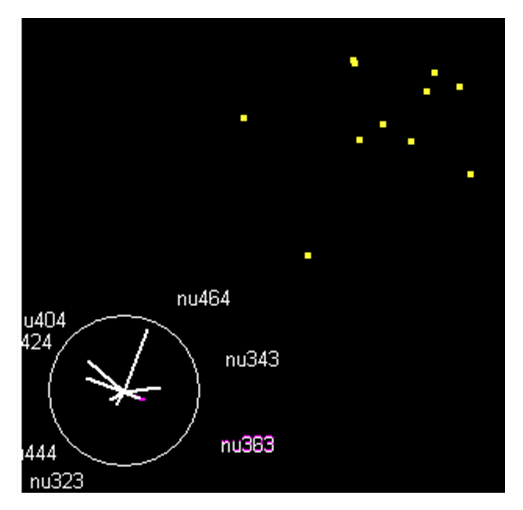
\includegraphics{2DTour_fcc.eps}
\caption[{G\footnotesize GOBI} snapshot of multidimensional fcc
RP�s.]{{G\footnotesize GOBI} snapshot of multidimensional fcc
RP�s. The axes are not located at the origin of the hypersphere,
which is approximately in the center of the group of RP's, but are
always located toward the lower left corner of the plot
window.}\label{2DTour}
\end{center}
\end{figure}

\begin{landscape}
\begin{figure}
\begin{center}
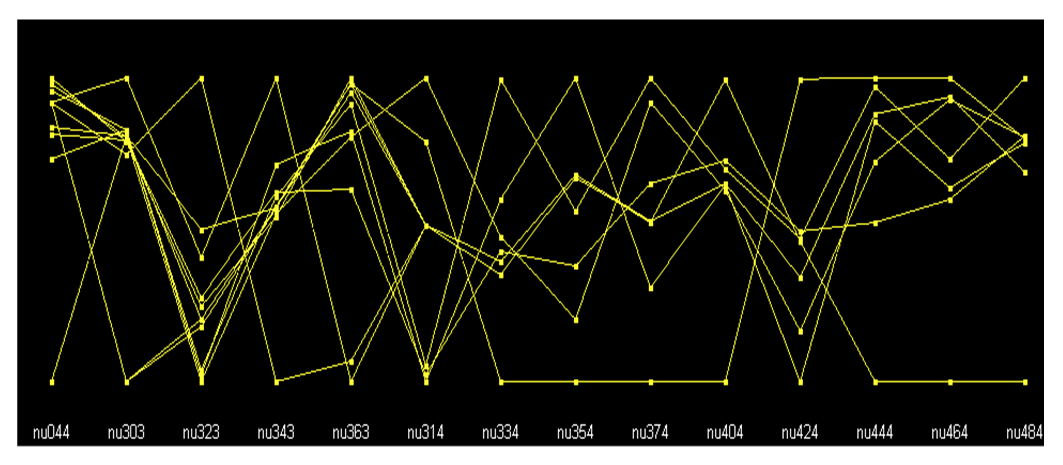
\includegraphics{parallelCoordinate_fcc.eps}
\caption[Parallel coordinate plot of fcc RP�s]{Parallel coordinate
plot of fcc RP�s.  Correlations in parameters nu044--nu363 show
preferred regions of potential parameter
space.}\label{parallelCoordinate}
\end{center}
\end{figure}
\end{landscape}

A parallel coordinate plot of the RPs is shown in
Fig.~\ref{parallelCoordinate}. The axes of each coordinate have
been normalized to the maximum and minimum $\mb{\nu}$ values to
better show correlations. These correlations are evident in
potential parameter ``clusters" in $\nu_{0,4,4}$ through
$\nu_{3,6,3}$. As the basis functions in the potential are also a
possible basis set for expansion of a trial wavefunction when
solving the Schr\"{o}dinger equation, one may infer from this
diagram that different molecules have similar wave function
coefficients. This may occur due to the low kinetic energy
configurations favored by the Schr\"{o}dinger equation.  These
configurations/basis functions have fewer oscillations and
therefore are strongly weighted even for a variety of molecules.

Interpreting the potential coefficients in Table~\ref{RPTop} is
analogous to describing multipole interactions. These multipoles
include contributions from all interaction modes and are not limited
to electrostatic  interactions. In the case of tetrahedral molecules
the octopole ($\ell_i=3$) is the first nonzero multipole.
Coefficients such as $\nu_{0,3,3}$ and $\nu_{0,4,4}$ where $\ell_i$
or $\ell_j$ is zero represent an octopole or hexadecapole
interacting with the zeroth pole and are the crystal field
coefficients. As the basis functions may also be used as quantum
basis sets, the $\mb{\nu}$ may be calculated \emph{ab initio} and
have been given physical interpretations via symmetry-adpated
perturbation theory~\cite{Avoird94}.  For instance, although
dispersion and induction force can be found in all components of
$\mb{\nu}$, electrostatic forces contribute only to
$\nu^{n_\sigma,n_\mu}_{\ell_i,\ell_i+\ell_j,\ell_j}$~\cite{Stone84}
such as $\nu_{3,6,3}$, $\nu_{3,7,4}$, and $\nu_{4,8,4}$.

One drawback of using the algorithm in
Sec.~\ref{Computational_Strategy} is that, by finding the maximum
energy difference between a phase and all others, the RP's of
neighboring phases tend to be spread apart.  This is because an RP
is a vector representing a region in a space, not a unique set of IP
parameters.  Homologous series of molecules (\emph{i.e.} CF$_4$,
CCl$_4$, CBr$_4$, CI$_4$) are expected to show trends in $\mb{\nu}$
space. If members of homologous series have different crystal
structures, then they have different RP's. However, different RP's
are widely spread by our algorithm. Therefore RP's of homologous
series are often widely spaced, even if the molecules are expected
to have similar intermolecular potentials. This hides the expected
trends among homologues.

Correlations are evident in reference lattice assignments.
%Examples include the
%$\mathrm{CX}_4$ series composed of five homologues,
%$\mathrm{CI}_4$ [CSD structure ZZZKDW01~\cite{Pohl82}],
%$\mathrm{CBr}_4$ [CSD structure CTBROM~\cite{More77}],
%$\mathrm{CCl}_4$ [CSD structure CARBTC~\cite{Piermarini73}],
%$\mathrm{CF}_4$ [CSD structure TFMETH02~\cite{Fitch93}],
%$\mathrm{CD}_4$, in five structures, 121a (ZZZKDW01), 15f,f,f,f
%(CTBROM), 14e (QUGBOJ), 15e (REKYUB), 64d,f (METHANEIII), that all
%pack in one reference lattice, fcc. An organometallic example is
An example of this is a series of molecules with molecular formula
$\mathrm{C}_{16}\mathrm{H}_{36}\mathrm{X}_{4}\mathrm{In}_4\mathrm{N}_4$
where $\mathrm{X}$ is Cl, Br, or I. The first two structures, 14e
MECKUA and 12i MECKOU,
%[CSD structure MECKUA~\cite{Grabowy00} and CSD structure MECKOU~\cite{Grabowy00}]
pack in an fcc reference lattice while
the last, 11e MECKIO, %[CSD structure MECKIO~\cite{Grabowy00}],
packs in a tetragonal reference lattice intermediate between fcc and
bcc which is slightly closer to the bcc reference lattice. This
indicates at least the translational part of homologue potentials is
similar and that small changes in the atomic constituency can
slightly alter the intermolecular potential (IP), but significantly
alter crystal structure. This is consistent with experience that
similar molecules often have very different crystal structures
despite similar intermolecular potentials. GPDs acknowledge this by
placing the seemingly disparate structures close to one another in
IP parameter space.

In Sec.~\ref{Reference_Phases} we noted that structures 195a and
197a were very similar to higher symmetry structures (215a and
217a). If the molecules remained tetrahedral then the crystal would
retain higher symmetry but the reported atomic coordinates indicate
a minor molecular distortion reducing the space group symmetry.
Assuming that the reported space group is correct, these structures
require a symmetry-breaking pathway from sc and bcc with a minimal
truncation manifold of $\ell_i^{\mathrm{max}}=6$ or 9 (depending on
the potential-dependent transition pathway taken). In contrast to
these high manifold requirements most pathways in
Tables~\ref{cubic}-\ref{mono} require a third or fourth manifold
basis set. In view of the success of finding RP's using only the two
first manifolds ($\ell_i^{\mathrm{max}}=3$ or 4) for all other
molecules in the data set, it seems unlikely such a large number of
rapidly oscillating basis functions would be required to properly
describe the intermolecular potential for these structures.  It
seems more likely that, barring a Jahn-Teller crystal distortion,
the crystal symmetry may have been underspecified when reported to
the CSD.

\subsection{Extensions and Features of the Methodology}
\label{extensions}

We now discuss some of the ways to improve the model and algorithms.
An issue affecting the numerical accuracy of the RP is how large a
library of alternate crystal structures is needed to localize the RP
in $\mb{\nu}$ space. In our previous work~\cite{Mettes04} we
considered just the high-symmetry point isotropy subgroups and in
this work have followed suit since these are the most
common~\cite{Stokes88}. Recall that space group IR's are indexed by
reciprocal space vectors~\cite{Kovalev93,Zak69}. There are the same
number of $\mb{k}$ points in reciprocal space as there are unit
cells in the crystal and there is a correspondence between $\mb{k}$
points and supercell patterns in the crystal. Experimental
structures are supercells in their reference lattice. As nearly all
experimental structures contain a relatively small number of
clustered parent lattice unit cells as sublattices,
symmetry-breaking occurs at $\mb{k}$ vectors corresponding to this
small cluster.  These are $\mb{k}$ vectors at high symmetry points
in the reference lattice Brillouin zone. If the experimental
structure has a unit cell which is large or flattened/elongated,
however, $\mb{k}$ vectors corresponding to this larger or
longer/flatter group of parent lattice unit cells will be on high
symmetry lines and planes. Tables \ref{restOfPathways1} and
\ref{restOfPathways2} show that some experimental structures contain
large or non-clustered parent lattice unit cells such as 15f,f,f,f
or 152b and their $\mb{k}$ vectors therefore are from high-symmetry
plane and line IR's. Although these cases are less common, such
isotropy subgroups could be included in the candidate lattices in
Sec.~\ref{collection}. Providing such additional structures in the
library would place additional constraints on the RP for the
observed structures and therefore further localize the RP for each
observed structure at the expense of a much larger library.

In Sec.~\ref{collection} we chose to consider only isotropy
subgroups with one occupied Wyckoff point. This is a commonly used
simplification.~\cite{Verwer98} We have also discarded coupled IR
isotropy subgroups for the same reason. Our method could be extended
to include library structures with multiple Wyckoff points and those
from coupled IRs, although the computational demands are much higher
because of the larger set of candidate lattices and so we do not
pursue it here. The effect would be to further localize the RPs of
each phase, again at the expense of a much larger library.

Although tetrahedral molecules are used in the current example to
reverse engineer the IP, any molecular point group could be used
without a dramatic increase in the number of potential
coefficients $\mb{\nu}$ in the first two non-trivial manifolds.
This is because the absence of IP coefficients in lower manifolds
for high-symmetry molecules is offset by the larger number of
parameters in higher manifolds. Consider the number of basis
functions in the first two non-trivial manifolds of $I_h$
(the icosahedral group) %, $T_d$ (the tetrahedral group),
and $C_1$ (the point group of no special symmetry). These are the
highest and lowest molecular point group symmetries, respectively.
The first three manifolds of $I_h$ containing a totally symmetric
molecular representation are the zeroth, sixth, and tenth manifolds.
The number of potential coefficients is seven on the sixth manifold,
$\{\nu_{6,0,6}^{1,1}$, $\nu_{6,2,6}^{1,1}$,
...$\nu_{6,12,6}^{1,1}\}$, eleven on the tenth manifold,
$\{\nu_{10,0,10}^{1,1}$, $\nu_{10,2,10}^{1,1}$,
...$\nu_{10,20,10}^{1,1}\}$, and seven for the cross manifolds,
$\{\nu_{6,4,10}^{1,1}$, $\nu_{6,6,10}^{1,1}$,
...$\nu_{6,16,10}^{1,1}\}$.  There are also two crystal field
coefficients, $\{\nu_{0,6,6}^{1,1}$, $\nu_{0,10,10}^{1,1}\}$, giving
a total of 27 potential coefficients for $I_h$.  For $C_1$ the first
three manifolds are the zeroth, first, and second. The coefficients
on the first manifold are $\{\nu_{1,0,1}^{n_\sigma,n_\mu}$,
$\nu_{1,2,1}^{n_\sigma,n_\mu}\}$. Although there are three copies of
the totally symmetric molecular representation on the first manifold
and therefore the molecular frame indices $\sigma$ and $\mu$ in
Eq.~\ref{re:eq:vij2} go over $\{1,2,3\}$, we are free to choose the
standard orientation for the molecule corresponding to Euler angles
$\{0,0,0\}$.  If it is chosen with the IP major axis parallel to the
laboratory z-axis then only one of these is nonzero. This leaves two
coefficients $\{\nu_{1,0,1}^{1,1}$, $\nu_{1,2,1}^{1,1}\}$. If the
molecular minor axis in the standard orientation is oriented
parallel to the laboratory x-axis only four of the $\sigma$ and
$\mu$ are nonzero in the second manifold. This leaves 48
coefficients on the second manifold,
$\{\nu_{2,0,2}^{n_\sigma,n_\mu}$, $\nu_{2,2,2}^{n_\sigma,n_\mu}$,
$\nu_{2,4,2}^{n_\sigma,n_\mu}\}$. With five additional crystal field
coefficients $\{\nu^{1,1}_{0,1,1}$, $\nu^{1,n_\mu}_{0,2,2}\}$ and
eight cross manifold coefficients $\{\nu^{1,n_\mu}_{1,1,2}$,
$\nu^{1,n_\mu}_{1,3,2}\}$ the total number of coefficients on the
first three manifolds of $C_1$ is 60, an increase of roughly twofold
from highly symmetrical $I_h$. This shows that although this method
has been applied to tetrahedral molecules, it is applicable to other
molecular point group symmetries with only a modest change in the
number parameters.

\begin{table}
\begin{center}
\caption[Comparison of truncation strategies in the intermolecular
potential.]{Comparison of the cumulative number of parameters in
potential for a truncation at a given manifold for two truncation
strategies and three molecular point
groups.}\label{tab:truncation}
\begin{tabular}{ccccccccc}
\multicolumn{4}{c}{Direct Truncation} & &\multicolumn{4}{c}{$\ell$ sum Truncation}\\
\cline{1-4}\cline{6-9}\\
$\ell_i$ & $C_1$ & $T_d$ & $I_h$ & & $\ell_i+\ell_j$ & $C_1$ &
$T_d$ & $I_h$\\
\cline{1-4}\cline{6-9}\\
0  & $^*$  & $^*$  & $^*$  & & 0  & $^*$  & $^*$ & $^*$ \\
1  & 3  & 0  & 0  & & 1  & 1  & 0 & 0 \\
2  & 60 & 0  & 0  & & 2  & 6  & 0 & 0 \\
3  &    & 5  & 0  & & 3  & 15 & 1 & 0 \\
4  &    & 10 & 0  & & 4  &    & 1 & 0 \\
6  &    &    & 8  & & 6  &    & 6 & 1 \\
10 &    &    & 19 & & 10 &    &   & 8 \\
\cline{1-4}\cline{6-9}\\
\end{tabular}
\end{center}
$^*$ There is one isotropic basis function for $\ell_i=\ell_j=0$
in each case, but it does not drive orientational ordering.
\end{table}

Throughout we have implemented a simple direct cutoff truncation
scheme in which a doubly infinite summation is cut off at a maximum
manifold number $\ell_i^\mathrm{max}$.  An alternative is the
manifold-sum cutoff in which we truncate such that $\ell_i+\ell_j\le
\ell^\mathrm{max}$. This truncation would include smoother functions
before more rapidly oscillating ones which is consistent with our
expectations of lower-energy electronic contributions to the
potential. Also the number of potential parameters increases at a
slower rate with this truncation. This is shown in
Table~\ref{tab:truncation} for both truncation schemes where we
compare the cumulative number of parameters for the $C_1$, $T_d$,
and $I_h$ point groups at different manifolds. The truncation method
used in this study is a square truncation of the double sum while
the alternative is a triangular truncation. The manifold sum
truncation adds new parameters into the potential more slowly than
single manifold truncation. Therefore, the 15 coefficients used here
are sufficient but may not be necessary. Further investigation of
global phase diagrams with $\ell$-sum truncation is needed to test
this hypothesis. This is important since lower dimensional GPDs
would be easier to construct and to use.

From the foregoing discussion we have seen 15 coefficients are
sufficient to reverse engineer our dataset of experimental
structures.  We have not investigated if a linear combination would
be better.  Principle component analysis could be used to identify
linear combinations of basis functions that better fit molecules. It
is possible that less than 15 coefficients are necessary.

%Although Table~\ref{RPTop} shows that a potential can be
%successfully reverse engineered which produces the experimentally
%observed structure with remarkably few terms,

%As noted in Sec.~\ref{truncation}, some of the molecules in
%Table~\ref{group_theory} break symmetry due to coupled IR's.
%Although examples of coupled IR's exist in nature, they are less
%common than single IR's~\cite{Hatch87}. From experience gained in
%creating GPD's, coupled order parameters typically exist in a
%region of parameter space \emph{one dimension lower} than the
%surrounding phases. An example in 3D is that the coupled IR phase
%is the \emph{line} separating single IR \emph{surfaces} on the
%unit sphere. GPD calculations show phases with coupled IR's
%possess \emph{significantly} lower free energies than adjacent
%neighbors. An important consequence in crystal structure
%prediction is an interaction potential sufficient to produce one
%of these structures requires a very precise $\mb{\nu}$ vector.
%This may be an important contributor to the lack of success of
%crystal structure prediction codes~\cite{Motherwell02}. It also
%underscores the utility of GPD's in accurately assessing
%intermolecular forces.

\subsection{Conclusions}

We have shown that a molecular crystal global phase diagram (GPD)
can summarize the experimental data using a modest number of
reference lattices and IP parameters. In previous
work~\cite{Keith04c,Mettes04}, we somewhat arbitrarily chose a
single reference lattice (fcc) and truncated the intermolecular
potential with three terms to illustrate the method. Here, we have
used an experimental data set of crystals of tetrahedral molecules
to determine reference lattices and an IP truncation sufficient to
produce the observed phases. The data set is diverse enough to
test the GPD's ability to classify a wide range of space groups
using a common intermolecular potential. Just as the van
Konynenburg global phase diagram classification based on the
simple van der Waals equation of state is nonetheless widely used
to classify the phase behavior of real binary mixtures, molecular
crystal global phase diagrams may be useful in elucidating phase
behavior of a variety of real substances and, in turn, used to
develop novel intermolecular potentials and materials.

\section*{Acknowledgments}

This work received financial support from the American Chemical
Society - Petroleum Research Fund (PRF \#41774-AC10).
%
Computational resources maintained by the University of Minnesota
Supercomputer Institute were used for portions of this research.

\section*{Appendix}
\label{cartRot}

The cartesian rotation matrix,
\begin{eqnarray}
\mb{R}(a,\mb{\omega})=a\left(\begin{array}{c}\cos(\alpha)\cos(\beta)\cos(\gamma)
- \sin(\alpha))\sin(\gamma) \\
\cos(\beta)\cos(\gamma)\sin(\alpha) + \cos(\alpha)\sin(\gamma) \\
    -\cos(\gamma) \sin(\beta),\end{array} \right. \nonumber\\
%
\begin{array}{c}-\cos(\gamma)\sin(\alpha)-\cos(\alpha) \cos(\beta) \sin(\gamma)\\
\cos(\alpha)\cos(\gamma) - \cos(\beta)\sin(\alpha)\sin(\gamma) \\
    \sin(\beta) \sin(\gamma),\end{array} \nonumber\\
%
\left. \begin{array}{c}\cos(\alpha) \sin(\beta)\\
\sin(\alpha) \sin(\beta)\\
    \cos(\beta)\end{array}\right)
\end{eqnarray}
is produced by converting spherical coordinate Wigner functions to
cartesian coordinates.

%\begin{landscape}
%\begin{equation}
%\mb{R}=a\left(\begin{array}{ccc}\cos(\alpha)\cos(\beta)\cos(\gamma)
%- \sin(\alpha))\sin(\gamma) &
%-\cos(\gamma)\sin(\alpha)-\cos(\alpha) \cos(\beta) \sin(\gamma)&\cos(\alpha) \sin(\beta)\\
%\cos(\beta)\cos(\gamma)\sin(\alpha) + \cos(\alpha)\sin(\gamma) &
%\cos(\alpha)\cos(\gamma) - \cos(\beta)\sin(\alpha)\sin(\gamma) & \sin(\alpha) \sin(\beta)\\
%    -\cos(\gamma) \sin(\beta), \sin(\beta) \sin(\gamma),
%    \cos(\beta)\end{array}\right)
%\end{equation}
%\end{landscape}

     %-------------------------------------------------------------------------
     % The back matter of the paper - acknowledgements and references
     %-------------------------------------------------------------------------

     % Acknowledgements come after the appendices

\vfill \eject
% Create the reference section using BibTeX:
\bibliographystyle{normalTitle}
\bibliography{thesisbib}
